\documentclass[../Main.tex]{subfiles}

\begin{document}
\chapter{椭圆曲线列表}

\intro{
    介绍椭圆曲线的列表
}

\section{椭圆曲线列表}
枚举椭圆曲线列表
\begin{enumerate}
\item   secp112r1 : SECG/WTLS curve over a 112 bit prime field
\item   secp112r2 : SECG curve over a 112 bit prime field
\item   secp128r1 : SECG curve over a 128 bit prime field
\item   secp128r2 : SECG curve over a 128 bit prime field
\item   secp160k1 : SECG curve over a 160 bit prime field
\item   secp160r1 : SECG curve over a 160 bit prime field
\item   secp160r2 : SECG/WTLS curve over a 160 bit prime field
\item   secp192k1 : SECG curve over a 192 bit prime field
\item   secp224k1 : SECG curve over a 224 bit prime field
\item   secp224r1 : NIST/SECG curve over a 224 bit prime field
\item   secp256k1 : SECG curve over a 256 bit prime field
\item   secp384r1 : NIST/SECG curve over a 384 bit prime field
\item   secp521r1 : NIST/SECG curve over a 521 bit prime field
\item   prime192v1: NIST/X9.62/SECG curve over a 192 bit prime field
\item   prime192v2: X9.62 curve over a 192 bit prime field
\item   prime192v3: X9.62 curve over a 192 bit prime field
\item   prime239v1: X9.62 curve over a 239 bit prime field
\item   prime239v2: X9.62 curve over a 239 bit prime field
\item   prime239v3: X9.62 curve over a 239 bit prime field
\item   prime256v1: X9.62/SECG curve over a 256 bit prime field
\item   sect113r1 : SECG curve over a 113 bit binary field
\item   sect113r2 : SECG curve over a 113 bit binary field
\item   sect131r1 : SECG/WTLS curve over a 131 bit binary field
\item   sect131r2 : SECG curve over a 131 bit binary field
\item   sect163k1 : NIST/SECG/WTLS curve over a 163 bit binary field
\item   sect163r1 : SECG curve over a 163 bit binary field
\item   sect163r2 : NIST/SECG curve over a 163 bit binary field
\item   sect193r1 : SECG curve over a 193 bit binary field
\item   sect193r2 : SECG curve over a 193 bit binary field
\item   sect233k1 : NIST/SECG/WTLS curve over a 233 bit binary field
\item   sect233r1 : NIST/SECG/WTLS curve over a 233 bit binary field
\item   sect239k1 : SECG curve over a 239 bit binary field
\item   sect283k1 : NIST/SECG curve over a 283 bit binary field
\item   sect283r1 : NIST/SECG curve over a 283 bit binary field
\item   sect409k1 : NIST/SECG curve over a 409 bit binary field
\item   sect409r1 : NIST/SECG curve over a 409 bit binary field
\item   sect571k1 : NIST/SECG curve over a 571 bit binary field
\item   sect571r1 : NIST/SECG curve over a 571 bit binary field
\item   c2pnb163v1: X9.62 curve over a 163 bit binary field
\item   c2pnb163v2: X9.62 curve over a 163 bit binary field
\item   c2pnb163v3: X9.62 curve over a 163 bit binary field
\item   c2pnb176v1: X9.62 curve over a 176 bit binary field
\item   c2tnb191v1: X9.62 curve over a 191 bit binary field
\item   c2tnb191v2: X9.62 curve over a 191 bit binary field
\item   c2tnb191v3: X9.62 curve over a 191 bit binary field
\item   c2pnb208w1: X9.62 curve over a 208 bit binary field
\item   c2tnb239v1: X9.62 curve over a 239 bit binary field
\item   c2tnb239v2: X9.62 curve over a 239 bit binary field
\item   c2tnb239v3: X9.62 curve over a 239 bit binary field
\item   c2pnb272w1: X9.62 curve over a 272 bit binary field
\item   c2pnb304w1: X9.62 curve over a 304 bit binary field
\item   c2tnb359v1: X9.62 curve over a 359 bit binary field
\item   c2pnb368w1: X9.62 curve over a 368 bit binary field
\item   c2tnb431r1: X9.62 curve over a 431 bit binary field
\item   wap-wsg-idm-ecid-wtls1: WTLS curve over a 113 bit binary field
\item   wap-wsg-idm-ecid-wtls3: NIST/SECG/WTLS curve over a 163 bit binary field
\item   wap-wsg-idm-ecid-wtls4: SECG curve over a 113 bit binary field
\item   wap-wsg-idm-ecid-wtls5: X9.62 curve over a 163 bit binary field
\item   wap-wsg-idm-ecid-wtls6: SECG/WTLS curve over a 112 bit prime field
\item   wap-wsg-idm-ecid-wtls7: SECG/WTLS curve over a 160 bit prime field
\item   wap-wsg-idm-ecid-wtls8: WTLS curve over a 112 bit prime field
\item   wap-wsg-idm-ecid-wtls9: WTLS curve over a 160 bit prime field
\item   wap-wsg-idm-ecid-wtls10: NIST/SECG/WTLS curve over a 233 bit binary field
\item   wap-wsg-idm-ecid-wtls11: NIST/SECG/WTLS curve over a 233 bit binary field
\item   wap-wsg-idm-ecid-wtls12: WTLS curve over a 224 bit prime field
\item   Oakley-EC2N-3: \\
	IPSec/IKE/Oakley curve \#3 over a 155 bit binary field. \\
	Not suitable for ECDSA. \\
	Questionable extension field!
\item   Oakley-EC2N-4: \\
	IPSec/IKE/Oakley curve \#4 over a 185 bit binary field. \\
	Not suitable for ECDSA. \\
	Questionable extension field!
\item   brainpoolP160r1: RFC 5639 curve over a 160 bit prime field
\item   brainpoolP160t1: RFC 5639 curve over a 160 bit prime field
\item   brainpoolP192r1: RFC 5639 curve over a 192 bit prime field
\item   brainpoolP192t1: RFC 5639 curve over a 192 bit prime field
\item   brainpoolP224r1: RFC 5639 curve over a 224 bit prime field
\item   brainpoolP224t1: RFC 5639 curve over a 224 bit prime field
\item   brainpoolP256r1: RFC 5639 curve over a 256 bit prime field
\item   brainpoolP256t1: RFC 5639 curve over a 256 bit prime field
\item   brainpoolP320r1: RFC 5639 curve over a 320 bit prime field
\item   brainpoolP320t1: RFC 5639 curve over a 320 bit prime field
\item   brainpoolP384r1: RFC 5639 curve over a 384 bit prime field
\item   brainpoolP384t1: RFC 5639 curve over a 384 bit prime field
\item   brainpoolP512r1: RFC 5639 curve over a 512 bit prime field
\item   brainpoolP512t1: RFC 5639 curve over a 512 bit prime field
\item   SM2       : SM2 curve over a 256 bit prime field
\end{enumerate}

\section{椭圆曲线的详情展示}

\begin{enumerate}
\item \textbf{ secp112r1 }\\
EC-Parameters: (112 bit)\\
Field Type: prime-field\\
Prime:\\
    00:db:7c:2a:bf:62:e3:5e:66:80:76:be:ad:20:8b\\
A:   \\
    00:db:7c:2a:bf:62:e3:5e:66:80:76:be:ad:20:88\\
B:   \\
    65:9e:f8:ba:04:39:16:ee:de:89:11:70:2b:22\\
Generator (uncompressed):\\
    04:09:48:72:39:99:5a:5e:e7:6b:55:f9:c2:f0:98:\\
    a8:9c:e5:af:87:24:c0:a2:3e:0e:0f:f7:75:00\\
Order: \\
    00:db:7c:2a:bf:62:e3:5e:76:28:df:ac:65:61:c5\\
Cofactor:  1 (0x1)\\
\item \textbf{ secp112r2 }\\
EC-Parameters: (110 bit)\\
Field Type: prime-field\\
Prime:\\
    00:db:7c:2a:bf:62:e3:5e:66:80:76:be:ad:20:8b\\
A:   \\
    61:27:c2:4c:05:f3:8a:0a:aa:f6:5c:0e:f0:2c\\
B:   \\
    51:de:f1:81:5d:b5:ed:74:fc:c3:4c:85:d7:09\\
Generator (uncompressed):\\
    04:4b:a3:0a:b5:e8:92:b4:e1:64:9d:d0:92:86:43:\\
    ad:cd:46:f5:88:2e:37:47:de:f3:6e:95:6e:97\\
Order: \\
    36:df:0a:af:d8:b8:d7:59:7c:a1:05:20:d0:4b\\
Cofactor:  4 (0x4)\\
\item \textbf{ secp128r1 }\\
EC-Parameters: (128 bit)\\
Field Type: prime-field\\
Prime:\\
    00:ff:ff:ff:fd:ff:ff:ff:ff:ff:ff:ff:ff:ff:ff:\\
    ff:ff\\
A:   \\
    00:ff:ff:ff:fd:ff:ff:ff:ff:ff:ff:ff:ff:ff:ff:\\
    ff:fc\\
B:   \\
    00:e8:75:79:c1:10:79:f4:3d:d8:24:99:3c:2c:ee:\\
    5e:d3\\
Generator (uncompressed):\\
    04:16:1f:f7:52:8b:89:9b:2d:0c:28:60:7c:a5:2c:\\
    5b:86:cf:5a:c8:39:5b:af:eb:13:c0:2d:a2:92:dd:\\
    ed:7a:83\\
Order: \\
    00:ff:ff:ff:fe:00:00:00:00:75:a3:0d:1b:90:38:\\
    a1:15\\
Cofactor:  1 (0x1)\\
\item \textbf{ secp128r2 }\\
EC-Parameters: (126 bit)\\
Field Type: prime-field\\
Prime:\\
    00:ff:ff:ff:fd:ff:ff:ff:ff:ff:ff:ff:ff:ff:ff:\\
    ff:ff\\
A:   \\
    00:d6:03:19:98:d1:b3:bb:fe:bf:59:cc:9b:bf:f9:\\
    ae:e1\\
B:   \\
    5e:ee:fc:a3:80:d0:29:19:dc:2c:65:58:bb:6d:8a:\\
    5d\\
Generator (uncompressed):\\
    04:7b:6a:a5:d8:5e:57:29:83:e6:fb:32:a7:cd:eb:\\
    c1:40:27:b6:91:6a:89:4d:3a:ee:71:06:fe:80:5f:\\
    c3:4b:44\\
Order: \\
    3f:ff:ff:ff:7f:ff:ff:ff:be:00:24:72:06:13:b5:\\
    a3\\
Cofactor:  4 (0x4)\\
\item \textbf{ secp160k1 }\\
EC-Parameters: (161 bit)\\
Field Type: prime-field\\
Prime:\\
    00:ff:ff:ff:ff:ff:ff:ff:ff:ff:ff:ff:ff:ff:ff:\\
    ff:fe:ff:ff:ac:73\\
A:    0\\
B:    7 (0x7)\\
Generator (uncompressed):\\
    04:3b:4c:38:2c:e3:7a:a1:92:a4:01:9e:76:30:36:\\
    f4:f5:dd:4d:7e:bb:93:8c:f9:35:31:8f:dc:ed:6b:\\
    c2:82:86:53:17:33:c3:f0:3c:4f:ee\\
Order: \\
    01:00:00:00:00:00:00:00:00:00:01:b8:fa:16:df:\\
    ab:9a:ca:16:b6:b3\\
Cofactor:  1 (0x1)\\
\item \textbf{ secp160r1 }\\
EC-Parameters: (161 bit)\\
Field Type: prime-field\\
Prime:\\
    00:ff:ff:ff:ff:ff:ff:ff:ff:ff:ff:ff:ff:ff:ff:\\
    ff:ff:7f:ff:ff:ff\\
A:   \\
    00:ff:ff:ff:ff:ff:ff:ff:ff:ff:ff:ff:ff:ff:ff:\\
    ff:ff:7f:ff:ff:fc\\
B:   \\
    1c:97:be:fc:54:bd:7a:8b:65:ac:f8:9f:81:d4:d4:\\
    ad:c5:65:fa:45\\
Generator (uncompressed):\\
    04:4a:96:b5:68:8e:f5:73:28:46:64:69:89:68:c3:\\
    8b:b9:13:cb:fc:82:23:a6:28:55:31:68:94:7d:59:\\
    dc:c9:12:04:23:51:37:7a:c5:fb:32\\
Order: \\
    01:00:00:00:00:00:00:00:00:00:01:f4:c8:f9:27:\\
    ae:d3:ca:75:22:57\\
Cofactor:  1 (0x1)\\
\item \textbf{ secp160r2 }\\
EC-Parameters: (161 bit)\\
Field Type: prime-field\\
Prime:\\
    00:ff:ff:ff:ff:ff:ff:ff:ff:ff:ff:ff:ff:ff:ff:\\
    ff:fe:ff:ff:ac:73\\
A:   \\
    00:ff:ff:ff:ff:ff:ff:ff:ff:ff:ff:ff:ff:ff:ff:\\
    ff:fe:ff:ff:ac:70\\
B:   \\
    00:b4:e1:34:d3:fb:59:eb:8b:ab:57:27:49:04:66:\\
    4d:5a:f5:03:88:ba\\
Generator (uncompressed):\\
    04:52:dc:b0:34:29:3a:11:7e:1f:4f:f1:1b:30:f7:\\
    19:9d:31:44:ce:6d:fe:af:fe:f2:e3:31:f2:96:e0:\\
    71:fa:0d:f9:98:2c:fe:a7:d4:3f:2e\\
Order: \\
    01:00:00:00:00:00:00:00:00:00:00:35:1e:e7:86:\\
    a8:18:f3:a1:a1:6b\\
Cofactor:  1 (0x1)\\
\item \textbf{ secp192k1 }\\
EC-Parameters: (192 bit)\\
Field Type: prime-field\\
Prime:\\
    00:ff:ff:ff:ff:ff:ff:ff:ff:ff:ff:ff:ff:ff:ff:\\
    ff:ff:ff:ff:ff:fe:ff:ff:ee:37\\
A:    0\\
B:    3 (0x3)\\
Generator (uncompressed):\\
    04:db:4f:f1:0e:c0:57:e9:ae:26:b0:7d:02:80:b7:\\
    f4:34:1d:a5:d1:b1:ea:e0:6c:7d:9b:2f:2f:6d:9c:\\
    56:28:a7:84:41:63:d0:15:be:86:34:40:82:aa:88:\\
    d9:5e:2f:9d\\
Order: \\
    00:ff:ff:ff:ff:ff:ff:ff:ff:ff:ff:ff:fe:26:f2:\\
    fc:17:0f:69:46:6a:74:de:fd:8d\\
Cofactor:  1 (0x1)\\
\item \textbf{ secp224k1 }\\
EC-Parameters: (225 bit)\\
Field Type: prime-field\\
Prime:\\
    00:ff:ff:ff:ff:ff:ff:ff:ff:ff:ff:ff:ff:ff:ff:\\
    ff:ff:ff:ff:ff:ff:ff:ff:ff:fe:ff:ff:e5:6d\\
A:    0\\
B:    5 (0x5)\\
Generator (uncompressed):\\
    04:a1:45:5b:33:4d:f0:99:df:30:fc:28:a1:69:a4:\\
    67:e9:e4:70:75:a9:0f:7e:65:0e:b6:b7:a4:5c:7e:\\
    08:9f:ed:7f:ba:34:42:82:ca:fb:d6:f7:e3:19:f7:\\
    c0:b0:bd:59:e2:ca:4b:db:55:6d:61:a5\\
Order: \\
    01:00:00:00:00:00:00:00:00:00:00:00:00:00:01:\\
    dc:e8:d2:ec:61:84:ca:f0:a9:71:76:9f:b1:f7\\
Cofactor:  1 (0x1)\\
\item \textbf{ secp224r1 }\\
EC-Parameters: (224 bit)\\
Field Type: prime-field\\
Prime:\\
    00:ff:ff:ff:ff:ff:ff:ff:ff:ff:ff:ff:ff:ff:ff:\\
    ff:ff:00:00:00:00:00:00:00:00:00:00:00:01\\
A:   \\
    00:ff:ff:ff:ff:ff:ff:ff:ff:ff:ff:ff:ff:ff:ff:\\
    ff:fe:ff:ff:ff:ff:ff:ff:ff:ff:ff:ff:ff:fe\\
B:   \\
    00:b4:05:0a:85:0c:04:b3:ab:f5:41:32:56:50:44:\\
    b0:b7:d7:bf:d8:ba:27:0b:39:43:23:55:ff:b4\\
Generator (uncompressed):\\
    04:b7:0e:0c:bd:6b:b4:bf:7f:32:13:90:b9:4a:03:\\
    c1:d3:56:c2:11:22:34:32:80:d6:11:5c:1d:21:bd:\\
    37:63:88:b5:f7:23:fb:4c:22:df:e6:cd:43:75:a0:\\
    5a:07:47:64:44:d5:81:99:85:00:7e:34\\
Order: \\
    00:ff:ff:ff:ff:ff:ff:ff:ff:ff:ff:ff:ff:ff:ff:\\
    16:a2:e0:b8:f0:3e:13:dd:29:45:5c:5c:2a:3d\\
Cofactor:  1 (0x1)\\
\item \textbf{ secp256k1 }\\
EC-Parameters: (256 bit)\\
Field Type: prime-field\\
Prime:\\
    00:ff:ff:ff:ff:ff:ff:ff:ff:ff:ff:ff:ff:ff:ff:\\
    ff:ff:ff:ff:ff:ff:ff:ff:ff:ff:ff:ff:ff:fe:ff:\\
    ff:fc:2f\\
A:    0\\
B:    7 (0x7)\\
Generator (uncompressed):\\
    04:79:be:66:7e:f9:dc:bb:ac:55:a0:62:95:ce:87:\\
    0b:07:02:9b:fc:db:2d:ce:28:d9:59:f2:81:5b:16:\\
    f8:17:98:48:3a:da:77:26:a3:c4:65:5d:a4:fb:fc:\\
    0e:11:08:a8:fd:17:b4:48:a6:85:54:19:9c:47:d0:\\
    8f:fb:10:d4:b8\\
Order: \\
    00:ff:ff:ff:ff:ff:ff:ff:ff:ff:ff:ff:ff:ff:ff:\\
    ff:fe:ba:ae:dc:e6:af:48:a0:3b:bf:d2:5e:8c:d0:\\
    36:41:41\\
Cofactor:  1 (0x1)\\
\item \textbf{ secp384r1 }\\
EC-Parameters: (384 bit)\\
Field Type: prime-field\\
Prime:\\
    00:ff:ff:ff:ff:ff:ff:ff:ff:ff:ff:ff:ff:ff:ff:\\
    ff:ff:ff:ff:ff:ff:ff:ff:ff:ff:ff:ff:ff:ff:ff:\\
    ff:ff:fe:ff:ff:ff:ff:00:00:00:00:00:00:00:00:\\
    ff:ff:ff:ff\\
A:   \\
    00:ff:ff:ff:ff:ff:ff:ff:ff:ff:ff:ff:ff:ff:ff:\\
    ff:ff:ff:ff:ff:ff:ff:ff:ff:ff:ff:ff:ff:ff:ff:\\
    ff:ff:fe:ff:ff:ff:ff:00:00:00:00:00:00:00:00:\\
    ff:ff:ff:fc\\
B:   \\
    00:b3:31:2f:a7:e2:3e:e7:e4:98:8e:05:6b:e3:f8:\\
    2d:19:18:1d:9c:6e:fe:81:41:12:03:14:08:8f:50:\\
    13:87:5a:c6:56:39:8d:8a:2e:d1:9d:2a:85:c8:ed:\\
    d3:ec:2a:ef\\
Generator (uncompressed):\\
    04:aa:87:ca:22:be:8b:05:37:8e:b1:c7:1e:f3:20:\\
    ad:74:6e:1d:3b:62:8b:a7:9b:98:59:f7:41:e0:82:\\
    54:2a:38:55:02:f2:5d:bf:55:29:6c:3a:54:5e:38:\\
    72:76:0a:b7:36:17:de:4a:96:26:2c:6f:5d:9e:98:\\
    bf:92:92:dc:29:f8:f4:1d:bd:28:9a:14:7c:e9:da:\\
    31:13:b5:f0:b8:c0:0a:60:b1:ce:1d:7e:81:9d:7a:\\
    43:1d:7c:90:ea:0e:5f\\
Order: \\
    00:ff:ff:ff:ff:ff:ff:ff:ff:ff:ff:ff:ff:ff:ff:\\
    ff:ff:ff:ff:ff:ff:ff:ff:ff:ff:c7:63:4d:81:f4:\\
    37:2d:df:58:1a:0d:b2:48:b0:a7:7a:ec:ec:19:6a:\\
    cc:c5:29:73\\
Cofactor:  1 (0x1)\\
\item \textbf{ secp521r1 }\\
EC-Parameters: (521 bit)\\
Field Type: prime-field\\
Prime:\\
    01:ff:ff:ff:ff:ff:ff:ff:ff:ff:ff:ff:ff:ff:ff:\\
    ff:ff:ff:ff:ff:ff:ff:ff:ff:ff:ff:ff:ff:ff:ff:\\
    ff:ff:ff:ff:ff:ff:ff:ff:ff:ff:ff:ff:ff:ff:ff:\\
    ff:ff:ff:ff:ff:ff:ff:ff:ff:ff:ff:ff:ff:ff:ff:\\
    ff:ff:ff:ff:ff:ff\\
A:   \\
    01:ff:ff:ff:ff:ff:ff:ff:ff:ff:ff:ff:ff:ff:ff:\\
    ff:ff:ff:ff:ff:ff:ff:ff:ff:ff:ff:ff:ff:ff:ff:\\
    ff:ff:ff:ff:ff:ff:ff:ff:ff:ff:ff:ff:ff:ff:ff:\\
    ff:ff:ff:ff:ff:ff:ff:ff:ff:ff:ff:ff:ff:ff:ff:\\
    ff:ff:ff:ff:ff:fc\\
B:   \\
    51:95:3e:b9:61:8e:1c:9a:1f:92:9a:21:a0:b6:85:\\
    40:ee:a2:da:72:5b:99:b3:15:f3:b8:b4:89:91:8e:\\
    f1:09:e1:56:19:39:51:ec:7e:93:7b:16:52:c0:bd:\\
    3b:b1:bf:07:35:73:df:88:3d:2c:34:f1:ef:45:1f:\\
    d4:6b:50:3f:00\\
Generator (uncompressed):\\
    04:00:c6:85:8e:06:b7:04:04:e9:cd:9e:3e:cb:66:\\
    23:95:b4:42:9c:64:81:39:05:3f:b5:21:f8:28:af:\\
    60:6b:4d:3d:ba:a1:4b:5e:77:ef:e7:59:28:fe:1d:\\
    c1:27:a2:ff:a8:de:33:48:b3:c1:85:6a:42:9b:f9:\\
    7e:7e:31:c2:e5:bd:66:01:18:39:29:6a:78:9a:3b:\\
    c0:04:5c:8a:5f:b4:2c:7d:1b:d9:98:f5:44:49:57:\\
    9b:44:68:17:af:bd:17:27:3e:66:2c:97:ee:72:99:\\
    5e:f4:26:40:c5:50:b9:01:3f:ad:07:61:35:3c:70:\\
    86:a2:72:c2:40:88:be:94:76:9f:d1:66:50\\
Order: \\
    01:ff:ff:ff:ff:ff:ff:ff:ff:ff:ff:ff:ff:ff:ff:\\
    ff:ff:ff:ff:ff:ff:ff:ff:ff:ff:ff:ff:ff:ff:ff:\\
    ff:ff:ff:fa:51:86:87:83:bf:2f:96:6b:7f:cc:01:\\
    48:f7:09:a5:d0:3b:b5:c9:b8:89:9c:47:ae:bb:6f:\\
    b7:1e:91:38:64:09\\
Cofactor:  1 (0x1)\\
\item \textbf{ prime192v1 }\\
EC-Parameters: (192 bit)\\
Field Type: prime-field\\
Prime:\\
    00:ff:ff:ff:ff:ff:ff:ff:ff:ff:ff:ff:ff:ff:ff:\\
    ff:fe:ff:ff:ff:ff:ff:ff:ff:ff\\
A:   \\
    00:ff:ff:ff:ff:ff:ff:ff:ff:ff:ff:ff:ff:ff:ff:\\
    ff:fe:ff:ff:ff:ff:ff:ff:ff:fc\\
B:   \\
    64:21:05:19:e5:9c:80:e7:0f:a7:e9:ab:72:24:30:\\
    49:fe:b8:de:ec:c1:46:b9:b1\\
Generator (uncompressed):\\
    04:18:8d:a8:0e:b0:30:90:f6:7c:bf:20:eb:43:a1:\\
    88:00:f4:ff:0a:fd:82:ff:10:12:07:19:2b:95:ff:\\
    c8:da:78:63:10:11:ed:6b:24:cd:d5:73:f9:77:a1:\\
    1e:79:48:11\\
Order: \\
    00:ff:ff:ff:ff:ff:ff:ff:ff:ff:ff:ff:ff:99:de:\\
    f8:36:14:6b:c9:b1:b4:d2:28:31\\
Cofactor:  1 (0x1)\\
\item \textbf{ prime192v2 }\\
EC-Parameters: (192 bit)\\
Field Type: prime-field\\
Prime:\\
    00:ff:ff:ff:ff:ff:ff:ff:ff:ff:ff:ff:ff:ff:ff:\\
    ff:fe:ff:ff:ff:ff:ff:ff:ff:ff\\
A:   \\
    00:ff:ff:ff:ff:ff:ff:ff:ff:ff:ff:ff:ff:ff:ff:\\
    ff:fe:ff:ff:ff:ff:ff:ff:ff:fc\\
B:   \\
    00:cc:22:d6:df:b9:5c:6b:25:e4:9c:0d:63:64:a4:\\
    e5:98:0c:39:3a:a2:16:68:d9:53\\
Generator (uncompressed):\\
    04:ee:a2:ba:e7:e1:49:78:42:f2:de:77:69:cf:e9:\\
    c9:89:c0:72:ad:69:6f:48:03:4a:65:74:d1:1d:69:\\
    b6:ec:7a:67:2b:b8:2a:08:3d:f2:f2:b0:84:7d:e9:\\
    70:b2:de:15\\
Order: \\
    00:ff:ff:ff:ff:ff:ff:ff:ff:ff:ff:ff:fe:5f:b1:\\
    a7:24:dc:80:41:86:48:d8:dd:31\\
Cofactor:  1 (0x1)\\
\item \textbf{ prime192v3 }\\
EC-Parameters: (192 bit)\\
Field Type: prime-field\\
Prime:\\
    00:ff:ff:ff:ff:ff:ff:ff:ff:ff:ff:ff:ff:ff:ff:\\
    ff:fe:ff:ff:ff:ff:ff:ff:ff:ff\\
A:   \\
    00:ff:ff:ff:ff:ff:ff:ff:ff:ff:ff:ff:ff:ff:ff:\\
    ff:fe:ff:ff:ff:ff:ff:ff:ff:fc\\
B:   \\
    22:12:3d:c2:39:5a:05:ca:a7:42:3d:ae:cc:c9:47:\\
    60:a7:d4:62:25:6b:d5:69:16\\
Generator (uncompressed):\\
    04:7d:29:77:81:00:c6:5a:1d:a1:78:37:16:58:8d:\\
    ce:2b:8b:4a:ee:8e:22:8f:18:96:38:a9:0f:22:63:\\
    73:37:33:4b:49:dc:b6:6a:6d:c8:f9:97:8a:ca:76:\\
    48:a9:43:b0\\
Order: \\
    00:ff:ff:ff:ff:ff:ff:ff:ff:ff:ff:ff:ff:7a:62:\\
    d0:31:c8:3f:42:94:f6:40:ec:13\\
Cofactor:  1 (0x1)\\
\item \textbf{ prime239v1 }\\
EC-Parameters: (239 bit)\\
Field Type: prime-field\\
Prime:\\
    7f:ff:ff:ff:ff:ff:ff:ff:ff:ff:ff:ff:7f:ff:ff:\\
    ff:ff:ff:80:00:00:00:00:00:7f:ff:ff:ff:ff:ff\\
A:   \\
    7f:ff:ff:ff:ff:ff:ff:ff:ff:ff:ff:ff:7f:ff:ff:\\
    ff:ff:ff:80:00:00:00:00:00:7f:ff:ff:ff:ff:fc\\
B:   \\
    6b:01:6c:3b:dc:f1:89:41:d0:d6:54:92:14:75:ca:\\
    71:a9:db:2f:b2:7d:1d:37:79:61:85:c2:94:2c:0a\\
Generator (uncompressed):\\
    04:0f:fa:96:3c:dc:a8:81:6c:cc:33:b8:64:2b:ed:\\
    f9:05:c3:d3:58:57:3d:3f:27:fb:bd:3b:3c:b9:aa:\\
    af:7d:eb:e8:e4:e9:0a:5d:ae:6e:40:54:ca:53:0b:\\
    a0:46:54:b3:68:18:ce:22:6b:39:fc:cb:7b:02:f1:\\
    ae\\
Order: \\
    7f:ff:ff:ff:ff:ff:ff:ff:ff:ff:ff:ff:7f:ff:ff:\\
    9e:5e:9a:9f:5d:90:71:fb:d1:52:26:88:90:9d:0b\\
Cofactor:  1 (0x1)\\
\item \textbf{ prime239v2 }\\
EC-Parameters: (239 bit)\\
Field Type: prime-field\\
Prime:\\
    7f:ff:ff:ff:ff:ff:ff:ff:ff:ff:ff:ff:7f:ff:ff:\\
    ff:ff:ff:80:00:00:00:00:00:7f:ff:ff:ff:ff:ff\\
A:   \\
    7f:ff:ff:ff:ff:ff:ff:ff:ff:ff:ff:ff:7f:ff:ff:\\
    ff:ff:ff:80:00:00:00:00:00:7f:ff:ff:ff:ff:fc\\
B:   \\
    61:7f:ab:68:32:57:6c:bb:fe:d5:0d:99:f0:24:9c:\\
    3f:ee:58:b9:4b:a0:03:8c:7a:e8:4c:8c:83:2f:2c\\
Generator (uncompressed):\\
    04:38:af:09:d9:87:27:70:51:20:c9:21:bb:5e:9e:\\
    26:29:6a:3c:dc:f2:f3:57:57:a0:ea:fd:87:b8:30:\\
    e7:5b:01:25:e4:db:ea:0e:c7:20:6d:a0:fc:01:d9:\\
    b0:81:32:9f:b5:55:de:6e:f4:60:23:7d:ff:8b:e4:\\
    ba\\
Order: \\
    7f:ff:ff:ff:ff:ff:ff:ff:ff:ff:ff:ff:80:00:00:\\
    cf:a7:e8:59:43:77:d4:14:c0:38:21:bc:58:20:63\\
Cofactor:  1 (0x1)\\
\item \textbf{ prime239v3 }\\
EC-Parameters: (239 bit)\\
Field Type: prime-field\\
Prime:\\
    7f:ff:ff:ff:ff:ff:ff:ff:ff:ff:ff:ff:7f:ff:ff:\\
    ff:ff:ff:80:00:00:00:00:00:7f:ff:ff:ff:ff:ff\\
A:   \\
    7f:ff:ff:ff:ff:ff:ff:ff:ff:ff:ff:ff:7f:ff:ff:\\
    ff:ff:ff:80:00:00:00:00:00:7f:ff:ff:ff:ff:fc\\
B:   \\
    25:57:05:fa:2a:30:66:54:b1:f4:cb:03:d6:a7:50:\\
    a3:0c:25:01:02:d4:98:87:17:d9:ba:15:ab:6d:3e\\
Generator (uncompressed):\\
    04:67:68:ae:8e:18:bb:92:cf:cf:00:5c:94:9a:a2:\\
    c6:d9:48:53:d0:e6:60:bb:f8:54:b1:c9:50:5f:e9:\\
    5a:16:07:e6:89:8f:39:0c:06:bc:1d:55:2b:ad:22:\\
    6f:3b:6f:cf:e4:8b:6e:81:84:99:af:18:e3:ed:6c:\\
    f3\\
Order: \\
    7f:ff:ff:ff:ff:ff:ff:ff:ff:ff:ff:ff:7f:ff:ff:\\
    97:5d:eb:41:b3:a6:05:7c:3c:43:21:46:52:65:51\\
Cofactor:  1 (0x1)\\
\item \textbf{ prime256v1 }\\
EC-Parameters: (256 bit)\\
Field Type: prime-field\\
Prime:\\
    00:ff:ff:ff:ff:00:00:00:01:00:00:00:00:00:00:\\
    00:00:00:00:00:00:ff:ff:ff:ff:ff:ff:ff:ff:ff:\\
    ff:ff:ff\\
A:   \\
    00:ff:ff:ff:ff:00:00:00:01:00:00:00:00:00:00:\\
    00:00:00:00:00:00:ff:ff:ff:ff:ff:ff:ff:ff:ff:\\
    ff:ff:fc\\
B:   \\
    5a:c6:35:d8:aa:3a:93:e7:b3:eb:bd:55:76:98:86:\\
    bc:65:1d:06:b0:cc:53:b0:f6:3b:ce:3c:3e:27:d2:\\
    60:4b\\
Generator (uncompressed):\\
    04:6b:17:d1:f2:e1:2c:42:47:f8:bc:e6:e5:63:a4:\\
    40:f2:77:03:7d:81:2d:eb:33:a0:f4:a1:39:45:d8:\\
    98:c2:96:4f:e3:42:e2:fe:1a:7f:9b:8e:e7:eb:4a:\\
    7c:0f:9e:16:2b:ce:33:57:6b:31:5e:ce:cb:b6:40:\\
    68:37:bf:51:f5\\
Order: \\
    00:ff:ff:ff:ff:00:00:00:00:ff:ff:ff:ff:ff:ff:\\
    ff:ff:bc:e6:fa:ad:a7:17:9e:84:f3:b9:ca:c2:fc:\\
    63:25:51\\
Cofactor:  1 (0x1)\\
\item \textbf{ sect113r1 }\\
EC-Parameters: (113 bit)\\
Field Type: characteristic-two-field\\
Basis Type: tpBasis\\
Polynomial:\\
    02:00:00:00:00:00:00:00:00:00:00:00:00:02:01\\
A:   \\
    30:88:25:0c:a6:e7:c7:fe:64:9c:e8:58:20:f7\\
B:   \\
    00:e8:be:e4:d3:e2:26:07:44:18:8b:e0:e9:c7:23\\
Generator (uncompressed):\\
    04:00:9d:73:61:6f:35:f4:ab:14:07:d7:35:62:c1:\\
    0f:00:a5:28:30:27:79:58:ee:84:d1:31:5e:d3:18:\\
    86\\
Order: \\
    01:00:00:00:00:00:00:00:d9:cc:ec:8a:39:e5:6f\\
Cofactor:  2 (0x2)\\
\item \textbf{ sect113r2 }\\
EC-Parameters: (113 bit)\\
Field Type: characteristic-two-field\\
Basis Type: tpBasis\\
Polynomial:\\
    02:00:00:00:00:00:00:00:00:00:00:00:00:02:01\\
A:   \\
    68:99:18:db:ec:7e:5a:0d:d6:df:c0:aa:55:c7\\
B:   \\
    00:95:e9:a9:ec:9b:29:7b:d4:bf:36:e0:59:18:4f\\
Generator (uncompressed):\\
    04:01:a5:7a:6a:7b:26:ca:5e:f5:2f:cd:b8:16:47:\\
    97:00:b3:ad:c9:4e:d1:fe:67:4c:06:e6:95:ba:ba:\\
    1d\\
Order: \\
    01:00:00:00:00:00:00:01:08:78:9b:24:96:af:93\\
Cofactor:  2 (0x2)\\
\item \textbf{ sect131r1 }\\
EC-Parameters: (131 bit)\\
Field Type: characteristic-two-field\\
Basis Type: ppBasis\\
Polynomial:\\
    08:00:00:00:00:00:00:00:00:00:00:00:00:00:00:\\
    01:0d\\
A:   \\
    07:a1:1b:09:a7:6b:56:21:44:41:8f:f3:ff:8c:25:\\
    70:b8\\
B:   \\
    02:17:c0:56:10:88:4b:63:b9:c6:c7:29:16:78:f9:\\
    d3:41\\
Generator (uncompressed):\\
    04:00:81:ba:f9:1f:df:98:33:c4:0f:9c:18:13:43:\\
    63:83:99:07:8c:6e:7e:a3:8c:00:1f:73:c8:13:4b:\\
    1b:4e:f9:e1:50\\
Order: \\
    04:00:00:00:00:00:00:00:02:31:23:95:3a:94:64:\\
    b5:4d\\
Cofactor:  2 (0x2)\\
\item \textbf{ sect131r2 }\\
EC-Parameters: (131 bit)\\
Field Type: characteristic-two-field\\
Basis Type: ppBasis\\
Polynomial:\\
    08:00:00:00:00:00:00:00:00:00:00:00:00:00:00:\\
    01:0d\\
A:   \\
    03:e5:a8:89:19:d7:ca:fc:bf:41:5f:07:c2:17:65:\\
    73:b2\\
B:   \\
    04:b8:26:6a:46:c5:56:57:ac:73:4c:e3:8f:01:8f:\\
    21:92\\
Generator (uncompressed):\\
    04:03:56:dc:d8:f2:f9:50:31:ad:65:2d:23:95:1b:\\
    b3:66:a8:06:48:f0:6d:86:79:40:a5:36:6d:9e:26:\\
    5d:e9:eb:24:0f\\
Order: \\
    04:00:00:00:00:00:00:00:01:69:54:a2:33:04:9b:\\
    a9:8f\\
Cofactor:  2 (0x2)\\
\item \textbf{ sect163k1 }\\
EC-Parameters: (163 bit)\\
Field Type: characteristic-two-field\\
Basis Type: ppBasis\\
Polynomial:\\
    08:00:00:00:00:00:00:00:00:00:00:00:00:00:00:\\
    00:00:00:00:00:c9\\
A:    1 (0x1)\\
B:    1 (0x1)\\
Generator (uncompressed):\\
    04:02:fe:13:c0:53:7b:bc:11:ac:aa:07:d7:93:de:\\
    4e:6d:5e:5c:94:ee:e8:02:89:07:0f:b0:5d:38:ff:\\
    58:32:1f:2e:80:05:36:d5:38:cc:da:a3:d9\\
Order: \\
    04:00:00:00:00:00:00:00:00:00:02:01:08:a2:e0:\\
    cc:0d:99:f8:a5:ef\\
Cofactor:  2 (0x2)\\
\item \textbf{ sect163r1 }\\
EC-Parameters: (162 bit)\\
Field Type: characteristic-two-field\\
Basis Type: ppBasis\\
Polynomial:\\
    08:00:00:00:00:00:00:00:00:00:00:00:00:00:00:\\
    00:00:00:00:00:c9\\
A:   \\
    07:b6:88:2c:aa:ef:a8:4f:95:54:ff:84:28:bd:88:\\
    e2:46:d2:78:2a:e2\\
B:   \\
    07:13:61:2d:cd:dc:b4:0a:ab:94:6b:da:29:ca:91:\\
    f7:3a:f9:58:af:d9\\
Generator (uncompressed):\\
    04:03:69:97:96:97:ab:43:89:77:89:56:67:89:56:\\
    7f:78:7a:78:76:a6:54:00:43:5e:db:42:ef:af:b2:\\
    98:9d:51:fe:fc:e3:c8:09:88:f4:1f:f8:83\\
Order: \\
    03:ff:ff:ff:ff:ff:ff:ff:ff:ff:ff:48:aa:b6:89:\\
    c2:9c:a7:10:27:9b\\
Cofactor:  2 (0x2)\\
\item \textbf{ sect163r2 }\\
EC-Parameters: (163 bit)\\
Field Type: characteristic-two-field\\
Basis Type: ppBasis\\
Polynomial:\\
    08:00:00:00:00:00:00:00:00:00:00:00:00:00:00:\\
    00:00:00:00:00:c9\\
A:    1 (0x1)\\
B:   \\
    02:0a:60:19:07:b8:c9:53:ca:14:81:eb:10:51:2f:\\
    78:74:4a:32:05:fd\\
Generator (uncompressed):\\
    04:03:f0:eb:a1:62:86:a2:d5:7e:a0:99:11:68:d4:\\
    99:46:37:e8:34:3e:36:00:d5:1f:bc:6c:71:a0:09:\\
    4f:a2:cd:d5:45:b1:1c:5c:0c:79:73:24:f1\\
Order: \\
    04:00:00:00:00:00:00:00:00:00:02:92:fe:77:e7:\\
    0c:12:a4:23:4c:33\\
Cofactor:  2 (0x2)\\
\item \textbf{ sect193r1 }\\
EC-Parameters: (193 bit)\\
Field Type: characteristic-two-field\\
Basis Type: tpBasis\\
Polynomial:\\
    02:00:00:00:00:00:00:00:00:00:00:00:00:00:00:\\
    00:00:00:00:00:00:00:00:80:01\\
A:   \\
    17:85:8f:eb:7a:98:97:51:69:e1:71:f7:7b:40:87:\\
    de:09:8a:c8:a9:11:df:7b:01\\
B:   \\
    00:fd:fb:49:bf:e6:c3:a8:9f:ac:ad:aa:7a:1e:5b:\\
    bc:7c:c1:c2:e5:d8:31:47:88:14\\
Generator (uncompressed):\\
    04:01:f4:81:bc:5f:0f:f8:4a:74:ad:6c:df:6f:de:\\
    f4:bf:61:79:62:53:72:d8:c0:c5:e1:00:25:e3:99:\\
    f2:90:37:12:cc:f3:ea:9e:3a:1a:d1:7f:b0:b3:20:\\
    1b:6a:f7:ce:1b:05\\
Order: \\
    01:00:00:00:00:00:00:00:00:00:00:00:00:c7:f3:\\
    4a:77:8f:44:3a:cc:92:0e:ba:49\\
Cofactor:  2 (0x2)\\
\item \textbf{ sect193r2 }\\
EC-Parameters: (193 bit)\\
Field Type: characteristic-two-field\\
Basis Type: tpBasis\\
Polynomial:\\
    02:00:00:00:00:00:00:00:00:00:00:00:00:00:00:\\
    00:00:00:00:00:00:00:00:80:01\\
A:   \\
    01:63:f3:5a:51:37:c2:ce:3e:a6:ed:86:67:19:0b:\\
    0b:c4:3e:cd:69:97:77:02:70:9b\\
B:   \\
    00:c9:bb:9e:89:27:d4:d6:4c:37:7e:2a:b2:85:6a:\\
    5b:16:e3:ef:b7:f6:1d:43:16:ae\\
Generator (uncompressed):\\
    04:00:d9:b6:7d:19:2e:03:67:c8:03:f3:9e:1a:7e:\\
    82:ca:14:a6:51:35:0a:ae:61:7e:8f:01:ce:94:33:\\
    56:07:c3:04:ac:29:e7:de:fb:d9:ca:01:f5:96:f9:\\
    27:22:4c:de:cf:6c\\
Order: \\
    01:00:00:00:00:00:00:00:00:00:00:00:01:5a:ab:\\
    56:1b:00:54:13:cc:d4:ee:99:d5\\
Cofactor:  2 (0x2)\\
\item \textbf{ sect233k1 }\\
EC-Parameters: (232 bit)\\
Field Type: characteristic-two-field\\
Basis Type: tpBasis\\
Polynomial:\\
    02:00:00:00:00:00:00:00:00:00:00:00:00:00:00:\\
    00:00:00:00:00:04:00:00:00:00:00:00:00:00:01\\
A:    0\\
B:    1 (0x1)\\
Generator (uncompressed):\\
    04:01:72:32:ba:85:3a:7e:73:1a:f1:29:f2:2f:f4:\\
    14:95:63:a4:19:c2:6b:f5:0a:4c:9d:6e:ef:ad:61:\\
    26:01:db:53:7d:ec:e8:19:b7:f7:0f:55:5a:67:c4:\\
    27:a8:cd:9b:f1:8a:eb:9b:56:e0:c1:10:56:fa:e6:\\
    a3\\
Order: \\
    00:80:00:00:00:00:00:00:00:00:00:00:00:00:00:\\
    06:9d:5b:b9:15:bc:d4:6e:fb:1a:d5:f1:73:ab:df\\
Cofactor:  4 (0x4)\\
\item \textbf{ sect233r1 }\\
EC-Parameters: (233 bit)\\
Field Type: characteristic-two-field\\
Basis Type: tpBasis\\
Polynomial:\\
    02:00:00:00:00:00:00:00:00:00:00:00:00:00:00:\\
    00:00:00:00:00:04:00:00:00:00:00:00:00:00:01\\
A:    1 (0x1)\\
B:   \\
    66:64:7e:de:6c:33:2c:7f:8c:09:23:bb:58:21:3b:\\
    33:3b:20:e9:ce:42:81:fe:11:5f:7d:8f:90:ad\\
Generator (uncompressed):\\
    04:00:fa:c9:df:cb:ac:83:13:bb:21:39:f1:bb:75:\\
    5f:ef:65:bc:39:1f:8b:36:f8:f8:eb:73:71:fd:55:\\
    8b:01:00:6a:08:a4:19:03:35:06:78:e5:85:28:be:\\
    bf:8a:0b:ef:f8:67:a7:ca:36:71:6f:7e:01:f8:10:\\
    52\\
Order: \\
    01:00:00:00:00:00:00:00:00:00:00:00:00:00:00:\\
    13:e9:74:e7:2f:8a:69:22:03:1d:26:03:cf:e0:d7\\
Cofactor:  2 (0x2)\\
\item \textbf{ sect239k1 }\\
EC-Parameters: (238 bit)\\
Field Type: characteristic-two-field\\
Basis Type: tpBasis\\
Polynomial:\\
    00:80:00:00:00:00:00:00:00:00:00:40:00:00:00:\\
    00:00:00:00:00:00:00:00:00:00:00:00:00:00:00:\\
    01\\
A:    0\\
B:    1 (0x1)\\
Generator (uncompressed):\\
    04:29:a0:b6:a8:87:a9:83:e9:73:09:88:a6:87:27:\\
    a8:b2:d1:26:c4:4c:c2:cc:7b:2a:65:55:19:30:35:\\
    dc:76:31:08:04:f1:2e:54:9b:db:01:1c:10:30:89:\\
    e7:35:10:ac:b2:75:fc:31:2a:5d:c6:b7:65:53:f0:\\
    ca\\
Order: \\
    20:00:00:00:00:00:00:00:00:00:00:00:00:00:00:\\
    5a:79:fe:c6:7c:b6:e9:1f:1c:1d:a8:00:e4:78:a5\\
Cofactor:  4 (0x4)\\
\item \textbf{ sect283k1 }\\
EC-Parameters: (281 bit)\\
Field Type: characteristic-two-field\\
Basis Type: ppBasis\\
Polynomial:\\
    08:00:00:00:00:00:00:00:00:00:00:00:00:00:00:\\
    00:00:00:00:00:00:00:00:00:00:00:00:00:00:00:\\
    00:00:00:00:10:a1\\
A:    0\\
B:    1 (0x1)\\
Generator (uncompressed):\\
    04:05:03:21:3f:78:ca:44:88:3f:1a:3b:81:62:f1:\\
    88:e5:53:cd:26:5f:23:c1:56:7a:16:87:69:13:b0:\\
    c2:ac:24:58:49:28:36:01:cc:da:38:0f:1c:9e:31:\\
    8d:90:f9:5d:07:e5:42:6f:e8:7e:45:c0:e8:18:46:\\
    98:e4:59:62:36:4e:34:11:61:77:dd:22:59\\
Order: \\
    01:ff:ff:ff:ff:ff:ff:ff:ff:ff:ff:ff:ff:ff:ff:\\
    ff:ff:ff:e9:ae:2e:d0:75:77:26:5d:ff:7f:94:45:\\
    1e:06:1e:16:3c:61\\
Cofactor:  4 (0x4)\\
\item \textbf{ sect283r1 }\\
EC-Parameters: (282 bit)\\
Field Type: characteristic-two-field\\
Basis Type: ppBasis\\
Polynomial:\\
    08:00:00:00:00:00:00:00:00:00:00:00:00:00:00:\\
    00:00:00:00:00:00:00:00:00:00:00:00:00:00:00:\\
    00:00:00:00:10:a1\\
A:    1 (0x1)\\
B:   \\
    02:7b:68:0a:c8:b8:59:6d:a5:a4:af:8a:19:a0:30:\\
    3f:ca:97:fd:76:45:30:9f:a2:a5:81:48:5a:f6:26:\\
    3e:31:3b:79:a2:f5\\
Generator (uncompressed):\\
    04:05:f9:39:25:8d:b7:dd:90:e1:93:4f:8c:70:b0:\\
    df:ec:2e:ed:25:b8:55:7e:ac:9c:80:e2:e1:98:f8:\\
    cd:be:cd:86:b1:20:53:03:67:68:54:fe:24:14:1c:\\
    b9:8f:e6:d4:b2:0d:02:b4:51:6f:f7:02:35:0e:dd:\\
    b0:82:67:79:c8:13:f0:df:45:be:81:12:f4\\
Order: \\
    03:ff:ff:ff:ff:ff:ff:ff:ff:ff:ff:ff:ff:ff:ff:\\
    ff:ff:ff:ef:90:39:96:60:fc:93:8a:90:16:5b:04:\\
    2a:7c:ef:ad:b3:07\\
Cofactor:  2 (0x2)\\
\item \textbf{ sect409k1 }\\
EC-Parameters: (407 bit)\\
Field Type: characteristic-two-field\\
Basis Type: tpBasis\\
Polynomial:\\
    02:00:00:00:00:00:00:00:00:00:00:00:00:00:00:\\
    00:00:00:00:00:00:00:00:00:00:00:00:00:00:00:\\
    00:00:00:00:00:00:00:00:00:00:00:80:00:00:00:\\
    00:00:00:00:00:00:01\\
A:    0\\
B:    1 (0x1)\\
Generator (uncompressed):\\
    04:00:60:f0:5f:65:8f:49:c1:ad:3a:b1:89:0f:71:\\
    84:21:0e:fd:09:87:e3:07:c8:4c:27:ac:cf:b8:f9:\\
    f6:7c:c2:c4:60:18:9e:b5:aa:aa:62:ee:22:2e:b1:\\
    b3:55:40:cf:e9:02:37:46:01:e3:69:05:0b:7c:4e:\\
    42:ac:ba:1d:ac:bf:04:29:9c:34:60:78:2f:91:8e:\\
    a4:27:e6:32:51:65:e9:ea:10:e3:da:5f:6c:42:e9:\\
    c5:52:15:aa:9c:a2:7a:58:63:ec:48:d8:e0:28:6b\\
Order: \\
    7f:ff:ff:ff:ff:ff:ff:ff:ff:ff:ff:ff:ff:ff:ff:\\
    ff:ff:ff:ff:ff:ff:ff:ff:ff:ff:fe:5f:83:b2:d4:\\
    ea:20:40:0e:c4:55:7d:5e:d3:e3:e7:ca:5b:4b:5c:\\
    83:b8:e0:1e:5f:cf\\
Cofactor:  4 (0x4)\\
\item \textbf{ sect409r1 }\\
EC-Parameters: (409 bit)\\
Field Type: characteristic-two-field\\
Basis Type: tpBasis\\
Polynomial:\\
    02:00:00:00:00:00:00:00:00:00:00:00:00:00:00:\\
    00:00:00:00:00:00:00:00:00:00:00:00:00:00:00:\\
    00:00:00:00:00:00:00:00:00:00:00:80:00:00:00:\\
    00:00:00:00:00:00:01\\
A:    1 (0x1)\\
B:   \\
    21:a5:c2:c8:ee:9f:eb:5c:4b:9a:75:3b:7b:47:6b:\\
    7f:d6:42:2e:f1:f3:dd:67:47:61:fa:99:d6:ac:27:\\
    c8:a9:a1:97:b2:72:82:2f:6c:d5:7a:55:aa:4f:50:\\
    ae:31:7b:13:54:5f\\
Generator (uncompressed):\\
    04:01:5d:48:60:d0:88:dd:b3:49:6b:0c:60:64:75:\\
    62:60:44:1c:de:4a:f1:77:1d:4d:b0:1f:fe:5b:34:\\
    e5:97:03:dc:25:5a:86:8a:11:80:51:56:03:ae:ab:\\
    60:79:4e:54:bb:79:96:a7:00:61:b1:cf:ab:6b:e5:\\
    f3:2b:bf:a7:83:24:ed:10:6a:76:36:b9:c5:a7:bd:\\
    19:8d:01:58:aa:4f:54:88:d0:8f:38:51:4f:1f:df:\\
    4b:4f:40:d2:18:1b:36:81:c3:64:ba:02:73:c7:06\\
Order: \\
    01:00:00:00:00:00:00:00:00:00:00:00:00:00:00:\\
    00:00:00:00:00:00:00:00:00:00:00:01:e2:aa:d6:\\
    a6:12:f3:33:07:be:5f:a4:7c:3c:9e:05:2f:83:81:\\
    64:cd:37:d9:a2:11:73\\
Cofactor:  2 (0x2)\\
\item \textbf{ sect571k1 }\\
EC-Parameters: (570 bit)\\
Field Type: characteristic-two-field\\
Basis Type: ppBasis\\
Polynomial:\\
    08:00:00:00:00:00:00:00:00:00:00:00:00:00:00:\\
    00:00:00:00:00:00:00:00:00:00:00:00:00:00:00:\\
    00:00:00:00:00:00:00:00:00:00:00:00:00:00:00:\\
    00:00:00:00:00:00:00:00:00:00:00:00:00:00:00:\\
    00:00:00:00:00:00:00:00:00:00:04:25\\
A:    0\\
B:    1 (0x1)\\
Generator (uncompressed):\\
    04:02:6e:b7:a8:59:92:3f:bc:82:18:96:31:f8:10:\\
    3f:e4:ac:9c:a2:97:00:12:d5:d4:60:24:80:48:01:\\
    84:1c:a4:43:70:95:84:93:b2:05:e6:47:da:30:4d:\\
    b4:ce:b0:8c:bb:d1:ba:39:49:47:76:fb:98:8b:47:\\
    17:4d:ca:88:c7:e2:94:52:83:a0:1c:89:72:03:49:\\
    dc:80:7f:4f:bf:37:4f:4a:ea:de:3b:ca:95:31:4d:\\
    d5:8c:ec:9f:30:7a:54:ff:c6:1e:fc:00:6d:8a:2c:\\
    9d:49:79:c0:ac:44:ae:a7:4f:be:bb:b9:f7:72:ae:\\
    dc:b6:20:b0:1a:7b:a7:af:1b:32:04:30:c8:59:19:\\
    84:f6:01:cd:4c:14:3e:f1:c7:a3\\
Order: \\
    02:00:00:00:00:00:00:00:00:00:00:00:00:00:00:\\
    00:00:00:00:00:00:00:00:00:00:00:00:00:00:00:\\
    00:00:00:00:00:00:13:18:50:e1:f1:9a:63:e4:b3:\\
    91:a8:db:91:7f:41:38:b6:30:d8:4b:e5:d6:39:38:\\
    1e:91:de:b4:5c:fe:77:8f:63:7c:10:01\\
Cofactor:  4 (0x4)\\
\item \textbf{ sect571r1 }\\
EC-Parameters: (570 bit)\\
Field Type: characteristic-two-field\\
Basis Type: ppBasis\\
Polynomial:\\
    08:00:00:00:00:00:00:00:00:00:00:00:00:00:00:\\
    00:00:00:00:00:00:00:00:00:00:00:00:00:00:00:\\
    00:00:00:00:00:00:00:00:00:00:00:00:00:00:00:\\
    00:00:00:00:00:00:00:00:00:00:00:00:00:00:00:\\
    00:00:00:00:00:00:00:00:00:00:04:25\\
A:    1 (0x1)\\
B:   \\
    02:f4:0e:7e:22:21:f2:95:de:29:71:17:b7:f3:d6:\\
    2f:5c:6a:97:ff:cb:8c:ef:f1:cd:6b:a8:ce:4a:9a:\\
    18:ad:84:ff:ab:bd:8e:fa:59:33:2b:e7:ad:67:56:\\
    a6:6e:29:4a:fd:18:5a:78:ff:12:aa:52:0e:4d:e7:\\
    39:ba:ca:0c:7f:fe:ff:7f:29:55:72:7a\\
Generator (uncompressed):\\
    04:03:03:00:1d:34:b8:56:29:6c:16:c0:d4:0d:3c:\\
    d7:75:0a:93:d1:d2:95:5f:a8:0a:a5:f4:0f:c8:db:\\
    7b:2a:bd:bd:e5:39:50:f4:c0:d2:93:cd:d7:11:a3:\\
    5b:67:fb:14:99:ae:60:03:86:14:f1:39:4a:bf:a3:\\
    b4:c8:50:d9:27:e1:e7:76:9c:8e:ec:2d:19:03:7b:\\
    f2:73:42:da:63:9b:6d:cc:ff:fe:b7:3d:69:d7:8c:\\
    6c:27:a6:00:9c:bb:ca:19:80:f8:53:39:21:e8:a6:\\
    84:42:3e:43:ba:b0:8a:57:62:91:af:8f:46:1b:b2:\\
    a8:b3:53:1d:2f:04:85:c1:9b:16:e2:f1:51:6e:23:\\
    dd:3c:1a:48:27:af:1b:8a:c1:5b\\
Order: \\
    03:ff:ff:ff:ff:ff:ff:ff:ff:ff:ff:ff:ff:ff:ff:\\
    ff:ff:ff:ff:ff:ff:ff:ff:ff:ff:ff:ff:ff:ff:ff:\\
    ff:ff:ff:ff:ff:ff:e6:61:ce:18:ff:55:98:73:08:\\
    05:9b:18:68:23:85:1e:c7:dd:9c:a1:16:1d:e9:3d:\\
    51:74:d6:6e:83:82:e9:bb:2f:e8:4e:47\\
Cofactor:  2 (0x2)\\
\item \textbf{ c2pnb163v1 }\\
EC-Parameters: (163 bit)\\
Field Type: characteristic-two-field\\
Basis Type: ppBasis\\
Polynomial:\\
    08:00:00:00:00:00:00:00:00:00:00:00:00:00:00:\\
    00:00:00:00:01:07\\
A:   \\
    07:25:46:b5:43:52:34:a4:22:e0:78:96:75:f4:32:\\
    c8:94:35:de:52:42\\
B:   \\
    00:c9:51:7d:06:d5:24:0d:3c:ff:38:c7:4b:20:b6:\\
    cd:4d:6f:9d:d4:d9\\
Generator (uncompressed):\\
    04:07:af:69:98:95:46:10:3d:79:32:9f:cc:3d:74:\\
    88:0f:33:bb:e8:03:cb:01:ec:23:21:1b:59:66:ad:\\
    ea:1d:3f:87:f7:ea:58:48:ae:f0:b7:ca:9f\\
Order: \\
    04:00:00:00:00:00:00:00:00:00:01:e6:0f:c8:82:\\
    1c:c7:4d:ae:af:c1\\
Cofactor:  2 (0x2)\\
\item \textbf{ c2pnb163v2 }\\
EC-Parameters: (162 bit)\\
Field Type: characteristic-two-field\\
Basis Type: ppBasis\\
Polynomial:\\
    08:00:00:00:00:00:00:00:00:00:00:00:00:00:00:\\
    00:00:00:00:01:07\\
A:   \\
    01:08:b3:9e:77:c4:b1:08:be:d9:81:ed:0e:89:0e:\\
    11:7c:51:1c:f0:72\\
B:   \\
    06:67:ac:eb:38:af:4e:48:8c:40:74:33:ff:ae:4f:\\
    1c:81:16:38:df:20\\
Generator (uncompressed):\\
    04:00:24:26:6e:4e:b5:10:6d:0a:96:4d:92:c4:86:\\
    0e:26:71:db:9b:6c:c5:07:9f:68:4d:df:66:84:c5:\\
    cd:25:8b:38:90:02:1b:23:86:df:d1:9f:c5\\
Order: \\
    03:ff:ff:ff:ff:ff:ff:ff:ff:ff:fd:f6:4d:e1:15:\\
    1a:db:b7:8f:10:a7\\
Cofactor:  2 (0x2)\\
\item \textbf{ c2pnb163v3 }\\
EC-Parameters: (162 bit)\\
Field Type: characteristic-two-field\\
Basis Type: ppBasis\\
Polynomial:\\
    08:00:00:00:00:00:00:00:00:00:00:00:00:00:00:\\
    00:00:00:00:01:07\\
A:   \\
    07:a5:26:c6:3d:3e:25:a2:56:a0:07:69:9f:54:47:\\
    e3:2a:e4:56:b5:0e\\
B:   \\
    03:f7:06:17:98:eb:99:e2:38:fd:6f:1b:f9:5b:48:\\
    fe:eb:48:54:25:2b\\
Generator (uncompressed):\\
    04:02:f9:f8:7b:7c:57:4d:0b:de:cf:8a:22:e6:52:\\
    47:75:f9:8c:de:bd:cb:05:b9:35:59:0c:15:5e:17:\\
    ea:48:eb:3f:f3:71:8b:89:3d:f5:9a:05:d0\\
Order: \\
    03:ff:ff:ff:ff:ff:ff:ff:ff:ff:fe:1a:ee:14:0f:\\
    11:0a:ff:96:13:09\\
Cofactor:  2 (0x2)\\
\item \textbf{ c2pnb176v1 }\\
EC-Parameters: (161 bit)\\
Field Type: characteristic-two-field\\
Basis Type: ppBasis\\
Polynomial:\\
    01:00:00:00:00:00:00:00:00:00:00:00:00:00:00:\\
    00:00:08:00:00:00:00:07\\
A:   \\
    00:e4:e6:db:29:95:06:5c:40:7d:9d:39:b8:d0:96:\\
    7b:96:70:4b:a8:e9:c9:0b\\
B:   \\
    5d:da:47:0a:be:64:14:de:8e:c1:33:ae:28:e9:bb:\\
    d7:fc:ec:0a:e0:ff:f2\\
Generator (uncompressed):\\
    04:8d:16:c2:86:67:98:b6:00:f9:f0:8b:b4:a8:e8:\\
    60:f3:29:8c:e0:4a:57:98:6f:a4:53:9c:2d:ad:dd:\\
    d6:ba:b5:16:7d:61:b4:36:e1:d9:2b:b1:6a:56:2c\\
Order: \\
    01:00:92:53:73:97:ec:a4:f6:14:57:99:d6:2b:0a:\\
    19:ce:06:fe:26:ad\\
Cofactor:  65390 (0xff6e)\\
\item \textbf{ c2tnb191v1 }\\
EC-Parameters: (191 bit)\\
Field Type: characteristic-two-field\\
Basis Type: tpBasis\\
Polynomial:\\
    00:80:00:00:00:00:00:00:00:00:00:00:00:00:00:\\
    00:00:00:00:00:00:00:00:02:01\\
A:   \\
    28:66:53:7b:67:67:52:63:6a:68:f5:65:54:e1:26:\\
    40:27:6b:64:9e:f7:52:62:67\\
B:   \\
    2e:45:ef:57:1f:00:78:6f:67:b0:08:1b:94:95:a3:\\
    d9:54:62:f5:de:0a:a1:85:ec\\
Generator (uncompressed):\\
    04:36:b3:da:f8:a2:32:06:f9:c4:f2:99:d7:b2:1a:\\
    9c:36:91:37:f2:c8:4a:e1:aa:0d:76:5b:e7:34:33:\\
    b3:f9:5e:33:29:32:e7:0e:a2:45:ca:24:18:ea:0e:\\
    f9:80:18:fb\\
Order: \\
    40:00:00:00:00:00:00:00:00:00:00:00:04:a2:0e:\\
    90:c3:90:67:c8:93:bb:b9:a5\\
Cofactor:  2 (0x2)\\
\item \textbf{ c2tnb191v2 }\\
EC-Parameters: (190 bit)\\
Field Type: characteristic-two-field\\
Basis Type: tpBasis\\
Polynomial:\\
    00:80:00:00:00:00:00:00:00:00:00:00:00:00:00:\\
    00:00:00:00:00:00:00:00:02:01\\
A:   \\
    40:10:28:77:4d:77:77:c7:b7:66:6d:13:66:ea:43:\\
    20:71:27:4f:89:ff:01:e7:18\\
B:   \\
    06:20:04:8d:28:bc:bd:03:b6:24:9c:99:18:2b:7c:\\
    8c:d1:97:00:c3:62:c4:6a:01\\
Generator (uncompressed):\\
    04:38:09:b2:b7:cc:1b:28:cc:5a:87:92:6a:ad:83:\\
    fd:28:78:9e:81:e2:c9:e3:bf:10:17:43:43:86:62:\\
    6d:14:f3:db:f0:17:60:d9:21:3a:3e:1c:f3:7a:ec:\\
    43:7d:66:8a\\
Order: \\
    20:00:00:00:00:00:00:00:00:00:00:00:50:50:8c:\\
    b8:9f:65:28:24:e0:6b:81:73\\
Cofactor:  4 (0x4)\\
\item \textbf{ c2tnb191v3 }\\
EC-Parameters: (189 bit)\\
Field Type: characteristic-two-field\\
Basis Type: tpBasis\\
Polynomial:\\
    00:80:00:00:00:00:00:00:00:00:00:00:00:00:00:\\
    00:00:00:00:00:00:00:00:02:01\\
A:   \\
    6c:01:07:47:56:09:91:22:22:10:56:91:1c:77:d7:\\
    7e:77:a7:77:e7:e7:e7:7f:cb\\
B:   \\
    71:fe:1a:f9:26:cf:84:79:89:ef:ef:8d:b4:59:f6:\\
    63:94:d9:0f:32:ad:3f:15:e8\\
Generator (uncompressed):\\
    04:37:5d:4c:e2:4f:de:43:44:89:de:87:46:e7:17:\\
    86:01:50:09:e6:6e:38:a9:26:dd:54:5a:39:17:61:\\
    96:57:5d:98:59:99:36:6e:6a:d3:4c:e0:a7:7c:d7:\\
    12:7b:06:be\\
Order: \\
    15:55:55:55:55:55:55:55:55:55:55:55:61:0c:0b:\\
    19:68:12:bf:b6:28:8a:3e:a3\\
Cofactor:  6 (0x6)\\
\item \textbf{ c2pnb208w1 }\\
EC-Parameters: (193 bit)\\
Field Type: characteristic-two-field\\
Basis Type: ppBasis\\
Polynomial:\\
    01:00:00:00:00:00:00:00:00:00:00:00:00:00:00:\\
    00:08:00:00:00:00:00:00:00:00:00:07\\
A:    0\\
B:   \\
    00:c8:61:9e:d4:5a:62:e6:21:2e:11:60:34:9e:2b:\\
    fa:84:44:39:fa:fc:2a:3f:d1:63:8f:9e\\
Generator (uncompressed):\\
    04:89:fd:fb:e4:ab:e1:93:df:95:59:ec:f0:7a:c0:\\
    ce:78:55:4e:27:84:eb:8c:1e:d1:a5:7a:0f:55:b5:\\
    1a:06:e7:8e:9a:c3:8a:03:5f:f5:20:d8:b0:17:81:\\
    be:b1:a6:bb:08:61:7d:e3\\
Order: \\
    01:01:ba:f9:5c:97:23:c5:7b:6c:21:da:2e:ff:2d:\\
    5e:d5:88:bd:d5:71:7e:21:2f:9d\\
Cofactor:  65096 (0xfe48)\\
\item \textbf{ c2tnb239v1 }\\
EC-Parameters: (238 bit)\\
Field Type: characteristic-two-field\\
Basis Type: tpBasis\\
Polynomial:\\
    00:80:00:00:00:00:00:00:00:00:00:00:00:00:00:\\
    00:00:00:00:00:00:00:00:00:00:00:10:00:00:00:\\
    01\\
A:   \\
    32:01:08:57:07:7c:54:31:12:3a:46:b8:08:90:67:\\
    56:f5:43:42:3e:8d:27:87:75:78:12:57:78:ac:76\\
B:   \\
    79:04:08:f2:ee:da:f3:92:b0:12:ed:ef:b3:39:2f:\\
    30:f4:32:7c:0c:a3:f3:1f:c3:83:c4:22:aa:8c:16\\
Generator (uncompressed):\\
    04:57:92:70:98:fa:93:2e:7c:0a:96:d3:fd:5b:70:\\
    6e:f7:e5:f5:c1:56:e1:6b:7e:7c:86:03:85:52:e9:\\
    1d:61:d8:ee:50:77:c3:3f:ec:f6:f1:a1:6b:26:8d:\\
    e4:69:c3:c7:74:4e:a9:a9:71:64:9f:c7:a9:61:63:\\
    05\\
Order: \\
    20:00:00:00:00:00:00:00:00:00:00:00:00:00:00:\\
    0f:4d:42:ff:e1:49:2a:49:93:f1:ca:d6:66:e4:47\\
Cofactor:  4 (0x4)\\
\item \textbf{ c2tnb239v2 }\\
EC-Parameters: (237 bit)\\
Field Type: characteristic-two-field\\
Basis Type: tpBasis\\
Polynomial:\\
    00:80:00:00:00:00:00:00:00:00:00:00:00:00:00:\\
    00:00:00:00:00:00:00:00:00:00:00:10:00:00:00:\\
    01\\
A:   \\
    42:30:01:77:57:a7:67:fa:e4:23:98:56:9b:74:63:\\
    25:d4:53:13:af:07:66:26:64:79:b7:56:54:e6:5f\\
B:   \\
    50:37:ea:65:41:96:cf:f0:cd:82:b2:c1:4a:2f:cf:\\
    2e:3f:f8:77:52:85:b5:45:72:2f:03:ea:cd:b7:4b\\
Generator (uncompressed):\\
    04:28:f9:d0:4e:90:00:69:c8:dc:47:a0:85:34:fe:\\
    76:d2:b9:00:b7:d7:ef:31:f5:70:9f:20:0c:4c:a2:\\
    05:56:67:33:4c:45:af:f3:b5:a0:3b:ad:9d:d7:5e:\\
    2c:71:a9:93:62:56:7d:54:53:f7:fa:6e:22:7e:c8:\\
    33\\
Order: \\
    15:55:55:55:55:55:55:55:55:55:55:55:55:55:55:\\
    3c:6f:28:85:25:9c:31:e3:fc:df:15:46:24:52:2d\\
Cofactor:  6 (0x6)\\
\item \textbf{ c2tnb239v3 }\\
EC-Parameters: (236 bit)\\
Field Type: characteristic-two-field\\
Basis Type: tpBasis\\
Polynomial:\\
    00:80:00:00:00:00:00:00:00:00:00:00:00:00:00:\\
    00:00:00:00:00:00:00:00:00:00:00:10:00:00:00:\\
    01\\
A:   \\
    01:23:87:74:66:6a:67:76:6d:66:76:f7:78:e6:76:\\
    b6:69:99:17:66:66:e6:87:66:6d:87:66:c6:6a:9f\\
B:   \\
    6a:94:19:77:ba:9f:6a:43:51:99:ac:fc:51:06:7e:\\
    d5:87:f5:19:c5:ec:b5:41:b8:e4:41:11:de:1d:40\\
Generator (uncompressed):\\
    04:70:f6:e9:d0:4d:28:9c:4e:89:91:3c:e3:53:0b:\\
    fd:e9:03:97:7d:42:b1:46:d5:39:bf:1b:de:4e:9c:\\
    92:2e:5a:0e:af:6e:5e:13:05:b9:00:4d:ce:5c:0e:\\
    d7:fe:59:a3:56:08:f3:38:37:c8:16:d8:0b:79:f4:\\
    61\\
Order: \\
    0c:cc:cc:cc:cc:cc:cc:cc:cc:cc:cc:cc:cc:cc:cc:\\
    ac:49:12:d2:d9:df:90:3e:f9:88:8b:8a:0e:4c:ff\\
Cofactor:  10 (0xa)\\
\item \textbf{ c2pnb272w1 }\\
EC-Parameters: (257 bit)\\
Field Type: characteristic-two-field\\
Basis Type: ppBasis\\
Polynomial:\\
    01:00:00:00:00:00:00:00:00:00:00:00:00:00:00:\\
    00:00:00:00:00:00:00:00:00:00:00:00:01:00:00:\\
    00:00:00:00:0b\\
A:   \\
    00:91:a0:91:f0:3b:5f:ba:4a:b2:cc:f4:9c:4e:dd:\\
    22:0f:b0:28:71:2d:42:be:75:2b:2c:40:09:4d:ba:\\
    cd:b5:86:fb:20\\
B:   \\
    71:67:ef:c9:2b:b2:e3:ce:7c:8a:aa:ff:34:e1:2a:\\
    9c:55:70:03:d7:c7:3a:6f:af:00:3f:99:f6:cc:84:\\
    82:e5:40:f7\\
Generator (uncompressed):\\
    04:61:08:ba:bb:2c:ee:bc:f7:87:05:8a:05:6c:be:\\
    0c:fe:62:2d:77:23:a2:89:e0:8a:07:ae:13:ef:0d:\\
    10:d1:71:dd:8d:10:c7:69:57:16:85:1e:ef:6b:a7:\\
    f6:87:2e:61:42:fb:d2:41:b8:30:ff:5e:fc:ac:ec:\\
    ca:b0:5e:02:00:5d:de:9d:23\\
Order: \\
    01:00:fa:f5:13:54:e0:e3:9e:48:92:df:6e:31:9c:\\
    72:c8:16:16:03:fa:45:aa:7b:99:8a:16:7b:8f:1e:\\
    62:95:21\\
Cofactor:  65286 (0xff06)\\
\item \textbf{ c2pnb304w1 }\\
EC-Parameters: (289 bit)\\
Field Type: characteristic-two-field\\
Basis Type: ppBasis\\
Polynomial:\\
    01:00:00:00:00:00:00:00:00:00:00:00:00:00:00:\\
    00:00:00:00:00:00:00:00:00:00:00:00:00:00:00:\\
    00:00:00:00:00:00:00:08:07\\
A:   \\
    00:fd:0d:69:31:49:a1:18:f6:51:e6:dc:e6:80:20:\\
    85:37:7e:5f:88:2d:1b:51:0b:44:16:00:74:c1:28:\\
    80:78:36:5a:03:96:c8:e6:81\\
B:   \\
    00:bd:db:97:e5:55:a5:0a:90:8e:43:b0:1c:79:8e:\\
    a5:da:a6:78:8f:1e:a2:79:4e:fc:f5:71:66:b8:c1:\\
    40:39:60:1e:55:82:73:40:be\\
Generator (uncompressed):\\
    04:19:7b:07:84:5e:9b:e2:d9:6a:db:0f:5f:3c:7f:\\
    2c:ff:bd:7a:3e:b8:b6:fe:c3:5c:7f:d6:7f:26:dd:\\
    f6:28:5a:64:4f:74:0a:26:14:e1:9f:be:b7:6e:0d:\\
    a1:71:51:7e:cf:40:1b:50:28:9b:f0:14:10:32:88:\\
    52:7a:9b:41:6a:10:5e:80:26:0b:54:9f:dc:1b:92:\\
    c0:3b\\
Order: \\
    01:01:d5:56:57:2a:ab:ac:80:01:01:d5:56:57:2a:\\
    ab:ac:80:01:02:2d:5c:91:dd:17:3f:8f:b5:61:da:\\
    68:99:16:44:43:05:1d\\
Cofactor:  65070 (0xfe2e)\\
\item \textbf{ c2tnb359v1 }\\
EC-Parameters: (353 bit)\\
Field Type: characteristic-two-field\\
Basis Type: tpBasis\\
Polynomial:\\
    00:80:00:00:00:00:00:00:00:00:00:00:00:00:00:\\
    00:00:00:00:00:00:00:00:00:00:00:00:00:00:00:\\
    00:00:00:00:00:00:00:10:00:00:00:00:00:00:00:\\
    01\\
A:   \\
    56:67:67:6a:65:4b:20:75:4f:35:6e:a9:20:17:d9:\\
    46:56:7c:46:67:55:56:f1:95:56:a0:46:16:b5:67:\\
    d2:23:a5:e0:56:56:fb:54:90:16:a9:66:56:a5:57\\
B:   \\
    24:72:e2:d0:19:7c:49:36:3f:1f:e7:f5:b6:db:07:\\
    5d:52:b6:94:7d:13:5d:8c:a4:45:80:5d:39:bc:34:\\
    56:26:08:96:87:74:2b:63:29:e7:06:80:23:19:88\\
Generator (uncompressed):\\
    04:3c:25:8e:f3:04:77:67:e7:ed:e0:f1:fd:aa:79:\\
    da:ee:38:41:36:6a:13:2e:16:3a:ce:d4:ed:24:01:\\
    df:9c:6b:dc:de:98:e8:e7:07:c0:7a:22:39:b1:b0:\\
    97:53:d7:e0:85:29:54:70:48:12:1e:9c:95:f3:79:\\
    1d:d8:04:96:39:48:f3:4f:ae:7b:f4:4e:a8:23:65:\\
    dc:78:68:fe:57:e4:ae:2d:e2:11:30:5a:40:71:04:\\
    bd\\
Order: \\
    01:af:28:6b:ca:1a:f2:86:bc:a1:af:28:6b:ca:1a:\\
    f2:86:bc:a1:af:28:6b:c9:fb:8f:6b:85:c5:56:89:\\
    2c:20:a7:eb:96:4f:e7:71:9e:74:f4:90:75:8d:3b\\
Cofactor:  76 (0x4c)\\
\item \textbf{ c2pnb368w1 }\\
EC-Parameters: (353 bit)\\
Field Type: characteristic-two-field\\
Basis Type: ppBasis\\
Polynomial:\\
    01:00:00:00:00:00:00:00:00:00:00:00:00:00:00:\\
    00:00:00:00:00:00:00:00:00:00:00:00:00:00:00:\\
    00:00:00:00:00:00:20:00:00:00:00:00:00:00:00:\\
    00:07\\
A:   \\
    00:e0:d2:ee:25:09:52:06:f5:e2:a4:f9:ed:22:9f:\\
    1f:25:6e:79:a0:e2:b4:55:97:0d:8d:0d:86:5b:d9:\\
    47:78:c5:76:d6:2f:0a:b7:51:9c:cd:2a:1a:90:6a:\\
    e3:0d\\
B:   \\
    00:fc:12:17:d4:32:0a:90:45:2c:76:0a:58:ed:cd:\\
    30:c8:dd:06:9b:3c:34:45:38:37:a3:4e:d5:0c:b5:\\
    49:17:e1:c2:11:2d:84:d1:64:f4:44:f8:f7:47:86:\\
    04:6a\\
Generator (uncompressed):\\
    04:10:85:e2:75:53:81:dc:cc:e3:c1:55:7a:fa:10:\\
    c2:f0:c0:c2:82:56:46:c5:b3:4a:39:4c:bc:fa:8b:\\
    c1:6b:22:e7:e7:89:e9:27:be:21:6f:02:e1:fb:13:\\
    6a:5f:7b:3e:b1:bd:dc:ba:62:d5:d8:b2:05:9b:52:\\
    57:97:fc:73:82:2c:59:05:9c:62:3a:45:ff:38:43:\\
    ce:e8:f8:7c:d1:85:5a:da:a8:1e:2a:07:50:b8:0f:\\
    da:23:10\\
Order: \\
    01:00:90:51:2d:a9:af:72:b0:83:49:d9:8a:5d:d4:\\
    c7:b0:53:2e:ca:51:ce:03:e2:d1:0f:3b:7a:c5:79:\\
    bd:87:e9:09:ae:40:a6:f1:31:e9:cf:ce:5b:d9:67\\
Cofactor:  65392 (0xff70)\\
\item \textbf{ c2tnb431r1 }\\
EC-Parameters: (418 bit)\\
Field Type: characteristic-two-field\\
Basis Type: tpBasis\\
Polynomial:\\
    00:80:00:00:00:00:00:00:00:00:00:00:00:00:00:\\
    00:00:00:00:00:00:00:00:00:00:00:00:00:00:00:\\
    00:00:00:00:00:00:00:00:00:01:00:00:00:00:00:\\
    00:00:00:00:00:00:00:00:00:01\\
A:   \\
    1a:82:7e:f0:0d:d6:fc:0e:23:4c:af:04:6c:6a:5d:\\
    8a:85:39:5b:23:6c:c4:ad:2c:f3:2a:0c:ad:bd:c9:\\
    dd:f6:20:b0:eb:99:06:d0:95:7f:6c:6f:ea:cd:61:\\
    54:68:df:10:4d:e2:96:cd:8f\\
B:   \\
    10:d9:b4:a3:d9:04:7d:8b:15:43:59:ab:fb:1b:7f:\\
    54:85:b0:4c:eb:86:82:37:dd:c9:de:da:98:2a:67:\\
    9a:5a:91:9b:62:6d:4e:50:a8:dd:73:1b:10:7a:99:\\
    62:38:1f:b5:d8:07:bf:26:18\\
Generator (uncompressed):\\
    04:12:0f:c0:5d:3c:67:a9:9d:e1:61:d2:f4:09:26:\\
    22:fe:ca:70:1b:e4:f5:0f:47:58:71:4e:8a:87:bb:\\
    f2:a6:58:ef:8c:21:e7:c5:ef:e9:65:36:1f:6c:29:\\
    99:c0:c2:47:b0:db:d7:0c:e6:b7:20:d0:af:89:03:\\
    a9:6f:8d:5f:a2:c2:55:74:5d:3c:45:1b:30:2c:93:\\
    46:d9:b7:e4:85:e7:bc:e4:1f:6b:59:1f:3e:8f:6a:\\
    dd:cb:b0:bc:4c:2f:94:7a:7d:e1:a8:9b:62:5d:6a:\\
    59:8b:37:60\\
Order: \\
    03:40:34:03:40:34:03:40:34:03:40:34:03:40:34:\\
    03:40:34:03:40:34:03:40:34:03:40:34:03:23:c3:\\
    13:fa:b5:05:89:70:3b:5e:c6:8d:35:87:fe:c6:0d:\\
    16:1c:c1:49:c1:ad:4a:91\\
Cofactor:  10080 (0x2760)\\
\item \textbf{ wap-wsg-idm-ecid-wtls1 }\\
EC-Parameters: (112 bit)\\
Field Type: characteristic-two-field\\
Basis Type: tpBasis\\
Polynomial:\\
    02:00:00:00:00:00:00:00:00:00:00:00:00:02:01\\
A:    1 (0x1)\\
B:    1 (0x1)\\
Generator (uncompressed):\\
    04:01:66:79:79:a4:0b:a4:97:e5:d5:c2:70:78:06:\\
    17:00:f4:4b:4a:f1:ec:c2:63:0e:08:78:5c:eb:cc:\\
    15\\
Order: \\
    00:ff:ff:ff:ff:ff:ff:ff:fd:bf:91:af:6d:ea:73\\
Cofactor:  2 (0x2)\\
\item \textbf{ wap-wsg-idm-ecid-wtls3 }\\
EC-Parameters: (163 bit)\\
Field Type: characteristic-two-field\\
Basis Type: ppBasis\\
Polynomial:\\
    08:00:00:00:00:00:00:00:00:00:00:00:00:00:00:\\
    00:00:00:00:00:c9\\
A:    1 (0x1)\\
B:    1 (0x1)\\
Generator (uncompressed):\\
    04:02:fe:13:c0:53:7b:bc:11:ac:aa:07:d7:93:de:\\
    4e:6d:5e:5c:94:ee:e8:02:89:07:0f:b0:5d:38:ff:\\
    58:32:1f:2e:80:05:36:d5:38:cc:da:a3:d9\\
Order: \\
    04:00:00:00:00:00:00:00:00:00:02:01:08:a2:e0:\\
    cc:0d:99:f8:a5:ef\\
Cofactor:  2 (0x2)\\
\item \textbf{ wap-wsg-idm-ecid-wtls4 }\\
EC-Parameters: (113 bit)\\
Field Type: characteristic-two-field\\
Basis Type: tpBasis\\
Polynomial:\\
    02:00:00:00:00:00:00:00:00:00:00:00:00:02:01\\
A:   \\
    30:88:25:0c:a6:e7:c7:fe:64:9c:e8:58:20:f7\\
B:   \\
    00:e8:be:e4:d3:e2:26:07:44:18:8b:e0:e9:c7:23\\
Generator (uncompressed):\\
    04:00:9d:73:61:6f:35:f4:ab:14:07:d7:35:62:c1:\\
    0f:00:a5:28:30:27:79:58:ee:84:d1:31:5e:d3:18:\\
    86\\
Order: \\
    01:00:00:00:00:00:00:00:d9:cc:ec:8a:39:e5:6f\\
Cofactor:  2 (0x2)\\
\item \textbf{ wap-wsg-idm-ecid-wtls5 }\\
EC-Parameters: (163 bit)\\
Field Type: characteristic-two-field\\
Basis Type: ppBasis\\
Polynomial:\\
    08:00:00:00:00:00:00:00:00:00:00:00:00:00:00:\\
    00:00:00:00:01:07\\
A:   \\
    07:25:46:b5:43:52:34:a4:22:e0:78:96:75:f4:32:\\
    c8:94:35:de:52:42\\
B:   \\
    00:c9:51:7d:06:d5:24:0d:3c:ff:38:c7:4b:20:b6:\\
    cd:4d:6f:9d:d4:d9\\
Generator (uncompressed):\\
    04:07:af:69:98:95:46:10:3d:79:32:9f:cc:3d:74:\\
    88:0f:33:bb:e8:03:cb:01:ec:23:21:1b:59:66:ad:\\
    ea:1d:3f:87:f7:ea:58:48:ae:f0:b7:ca:9f\\
Order: \\
    04:00:00:00:00:00:00:00:00:00:01:e6:0f:c8:82:\\
    1c:c7:4d:ae:af:c1\\
Cofactor:  2 (0x2)\\
\item \textbf{ wap-wsg-idm-ecid-wtls6 }\\
EC-Parameters: (112 bit)\\
Field Type: prime-field\\
Prime:\\
    00:db:7c:2a:bf:62:e3:5e:66:80:76:be:ad:20:8b\\
A:   \\
    00:db:7c:2a:bf:62:e3:5e:66:80:76:be:ad:20:88\\
B:   \\
    65:9e:f8:ba:04:39:16:ee:de:89:11:70:2b:22\\
Generator (uncompressed):\\
    04:09:48:72:39:99:5a:5e:e7:6b:55:f9:c2:f0:98:\\
    a8:9c:e5:af:87:24:c0:a2:3e:0e:0f:f7:75:00\\
Order: \\
    00:db:7c:2a:bf:62:e3:5e:76:28:df:ac:65:61:c5\\
Cofactor:  1 (0x1)\\
\item \textbf{ wap-wsg-idm-ecid-wtls7 }\\
EC-Parameters: (161 bit)\\
Field Type: prime-field\\
Prime:\\
    00:ff:ff:ff:ff:ff:ff:ff:ff:ff:ff:ff:ff:ff:ff:\\
    ff:fe:ff:ff:ac:73\\
A:   \\
    00:ff:ff:ff:ff:ff:ff:ff:ff:ff:ff:ff:ff:ff:ff:\\
    ff:fe:ff:ff:ac:70\\
B:   \\
    00:b4:e1:34:d3:fb:59:eb:8b:ab:57:27:49:04:66:\\
    4d:5a:f5:03:88:ba\\
Generator (uncompressed):\\
    04:52:dc:b0:34:29:3a:11:7e:1f:4f:f1:1b:30:f7:\\
    19:9d:31:44:ce:6d:fe:af:fe:f2:e3:31:f2:96:e0:\\
    71:fa:0d:f9:98:2c:fe:a7:d4:3f:2e\\
Order: \\
    01:00:00:00:00:00:00:00:00:00:00:35:1e:e7:86:\\
    a8:18:f3:a1:a1:6b\\
Cofactor:  1 (0x1)\\
\item \textbf{ wap-wsg-idm-ecid-wtls8 }\\
EC-Parameters: (113 bit)\\
Field Type: prime-field\\
Prime:\\
    00:ff:ff:ff:ff:ff:ff:ff:ff:ff:ff:ff:ff:fd:e7\\
A:    0\\
B:    3 (0x3)\\
Generator (uncompressed):\\
    04:00:00:00:00:00:00:00:00:00:00:00:00:00:01:\\
    00:00:00:00:00:00:00:00:00:00:00:00:00:02\\
Order: \\
    01:00:00:00:00:00:00:01:ec:ea:55:1a:d8:37:e9\\
Cofactor:  1 (0x1)\\
\item \textbf{ wap-wsg-idm-ecid-wtls9 }\\
EC-Parameters: (161 bit)\\
Field Type: prime-field\\
Prime:\\
    00:ff:ff:ff:ff:ff:ff:ff:ff:ff:ff:ff:ff:ff:ff:\\
    ff:ff:ff:fc:80:8f\\
A:    0\\
B:    3 (0x3)\\
Generator (uncompressed):\\
    04:00:00:00:00:00:00:00:00:00:00:00:00:00:00:\\
    00:00:00:00:00:01:00:00:00:00:00:00:00:00:00:\\
    00:00:00:00:00:00:00:00:00:00:02\\
Order: \\
    01:00:00:00:00:00:00:00:00:00:01:cd:c9:8a:e0:\\
    e2:de:57:4a:bf:33\\
Cofactor:  1 (0x1)\\
\item \textbf{ wap-wsg-idm-ecid-wtls10 }\\
EC-Parameters: (232 bit)\\
Field Type: characteristic-two-field\\
Basis Type: tpBasis\\
Polynomial:\\
    02:00:00:00:00:00:00:00:00:00:00:00:00:00:00:\\
    00:00:00:00:00:04:00:00:00:00:00:00:00:00:01\\
A:    0\\
B:    1 (0x1)\\
Generator (uncompressed):\\
    04:01:72:32:ba:85:3a:7e:73:1a:f1:29:f2:2f:f4:\\
    14:95:63:a4:19:c2:6b:f5:0a:4c:9d:6e:ef:ad:61:\\
    26:01:db:53:7d:ec:e8:19:b7:f7:0f:55:5a:67:c4:\\
    27:a8:cd:9b:f1:8a:eb:9b:56:e0:c1:10:56:fa:e6:\\
    a3\\
Order: \\
    00:80:00:00:00:00:00:00:00:00:00:00:00:00:00:\\
    06:9d:5b:b9:15:bc:d4:6e:fb:1a:d5:f1:73:ab:df\\
Cofactor:  4 (0x4)\\
\item \textbf{ wap-wsg-idm-ecid-wtls11 }\\
EC-Parameters: (233 bit)\\
Field Type: characteristic-two-field\\
Basis Type: tpBasis\\
Polynomial:\\
    02:00:00:00:00:00:00:00:00:00:00:00:00:00:00:\\
    00:00:00:00:00:04:00:00:00:00:00:00:00:00:01\\
A:    1 (0x1)\\
B:   \\
    66:64:7e:de:6c:33:2c:7f:8c:09:23:bb:58:21:3b:\\
    33:3b:20:e9:ce:42:81:fe:11:5f:7d:8f:90:ad\\
Generator (uncompressed):\\
    04:00:fa:c9:df:cb:ac:83:13:bb:21:39:f1:bb:75:\\
    5f:ef:65:bc:39:1f:8b:36:f8:f8:eb:73:71:fd:55:\\
    8b:01:00:6a:08:a4:19:03:35:06:78:e5:85:28:be:\\
    bf:8a:0b:ef:f8:67:a7:ca:36:71:6f:7e:01:f8:10:\\
    52\\
Order: \\
    01:00:00:00:00:00:00:00:00:00:00:00:00:00:00:\\
    13:e9:74:e7:2f:8a:69:22:03:1d:26:03:cf:e0:d7\\
Cofactor:  2 (0x2)\\
\item \textbf{ wap-wsg-idm-ecid-wtls12 }\\
EC-Parameters: (224 bit)\\
Field Type: prime-field\\
Prime:\\
    00:ff:ff:ff:ff:ff:ff:ff:ff:ff:ff:ff:ff:ff:ff:\\
    ff:ff:00:00:00:00:00:00:00:00:00:00:00:01\\
A:   \\
    00:ff:ff:ff:ff:ff:ff:ff:ff:ff:ff:ff:ff:ff:ff:\\
    ff:fe:ff:ff:ff:ff:ff:ff:ff:ff:ff:ff:ff:fe\\
B:   \\
    00:b4:05:0a:85:0c:04:b3:ab:f5:41:32:56:50:44:\\
    b0:b7:d7:bf:d8:ba:27:0b:39:43:23:55:ff:b4\\
Generator (uncompressed):\\
    04:b7:0e:0c:bd:6b:b4:bf:7f:32:13:90:b9:4a:03:\\
    c1:d3:56:c2:11:22:34:32:80:d6:11:5c:1d:21:bd:\\
    37:63:88:b5:f7:23:fb:4c:22:df:e6:cd:43:75:a0:\\
    5a:07:47:64:44:d5:81:99:85:00:7e:34\\
Order: \\
    00:ff:ff:ff:ff:ff:ff:ff:ff:ff:ff:ff:ff:ff:ff:\\
    16:a2:e0:b8:f0:3e:13:dd:29:45:5c:5c:2a:3d\\
Cofactor:  1 (0x1)\\
\item \textbf{ Oakley-EC2N-3 }\\
EC-Parameters: (154 bit)\\
Field Type: characteristic-two-field\\
Basis Type: tpBasis\\
Polynomial:\\
    08:00:00:00:00:00:00:00:00:00:00:00:40:00:00:\\
    00:00:00:00:01\\
A:    0\\
B:    471951 (0x7338f)\\
Generator (uncompressed):\\
    04:00:00:00:00:00:00:00:00:00:00:00:00:00:00:\\
    00:00:00:00:00:7b:00:00:00:00:00:00:00:00:00:\\
    00:00:00:00:00:00:00:00:00:01:c8\\
Order: \\
    02:aa:aa:aa:aa:aa:aa:aa:aa:aa:c7:f3:c7:88:1b:\\
    d0:86:8f:a8:6c\\
Cofactor:  3 (0x3)\\
\item \textbf{ Oakley-EC2N-4 }\\
EC-Parameters: (184 bit)\\
Field Type: characteristic-two-field\\
Basis Type: tpBasis\\
Polynomial:\\
    02:00:00:00:00:00:00:00:00:00:00:00:00:00:00:\\
    20:00:00:00:00:00:00:00:01\\
A:    0\\
B:    7913 (0x1ee9)\\
Generator (uncompressed):\\
    04:00:00:00:00:00:00:00:00:00:00:00:00:00:00:\\
    00:00:00:00:00:00:00:00:00:18:00:00:00:00:00:\\
    00:00:00:00:00:00:00:00:00:00:00:00:00:00:00:\\
    00:00:00:0d\\
Order: \\
    00:ff:ff:ff:ff:ff:ff:ff:ff:ff:ff:ff:ed:f9:7c:\\
    44:db:9f:24:20:ba:fc:a7:5e\\
Cofactor:  2 (0x2)\\

\end{enumerate}

\section{椭圆曲线的绘图}
\begin{figure}[!htbp]

  \begin{minipage}{0.3\textwidth} \centering
    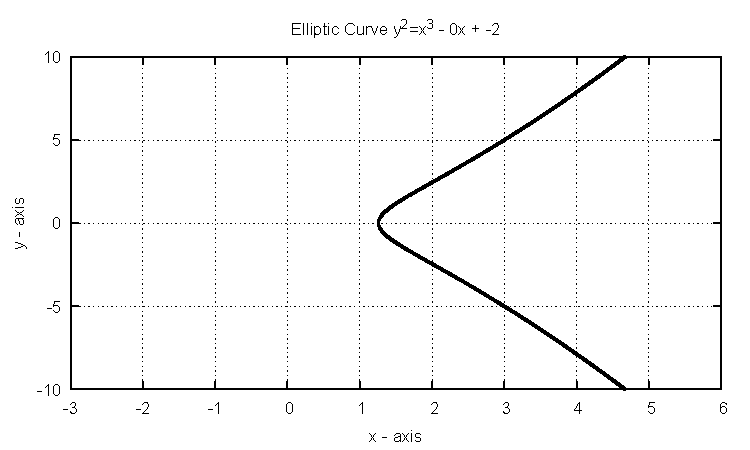
\includegraphics{../Images/ecc_plot/1}
  \end{minipage}
  \begin{minipage}{0.3\textwidth} \centering
    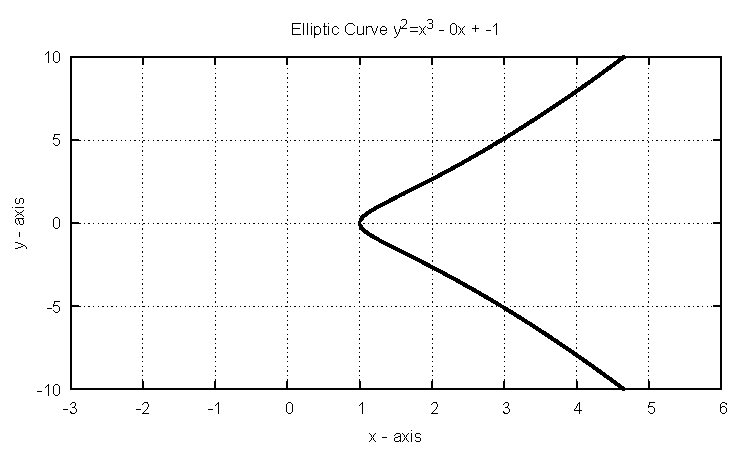
\includegraphics{../Images/ecc_plot/2}
  \end{minipage}
  \begin{minipage}{0.3\textwidth} \centering
    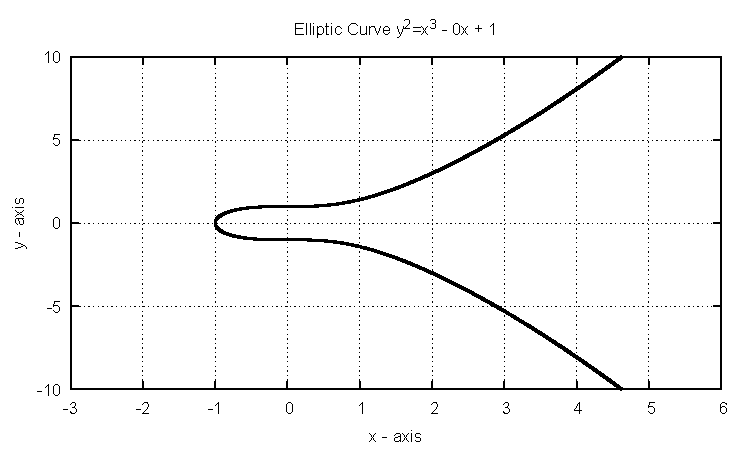
\includegraphics{../Images/ecc_plot/3}
  \end{minipage}
\end{figure}

\begin{figure}[!htbp]

  \begin{minipage}{0.3\textwidth} \centering
    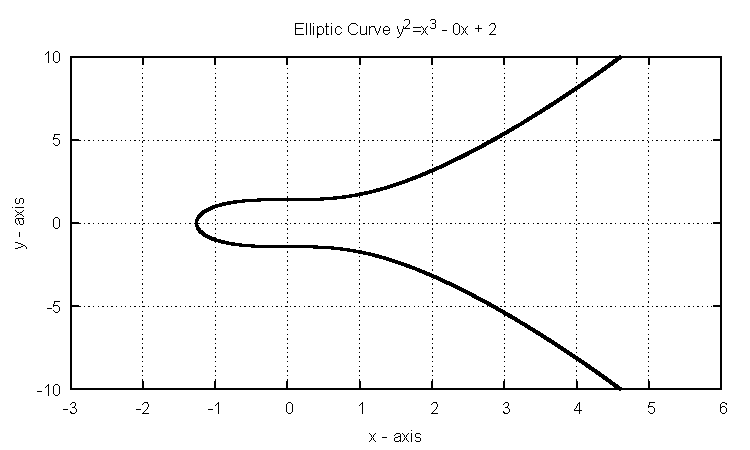
\includegraphics{../Images/ecc_plot/4}
  \end{minipage}
  \begin{minipage}{0.3\textwidth} \centering
    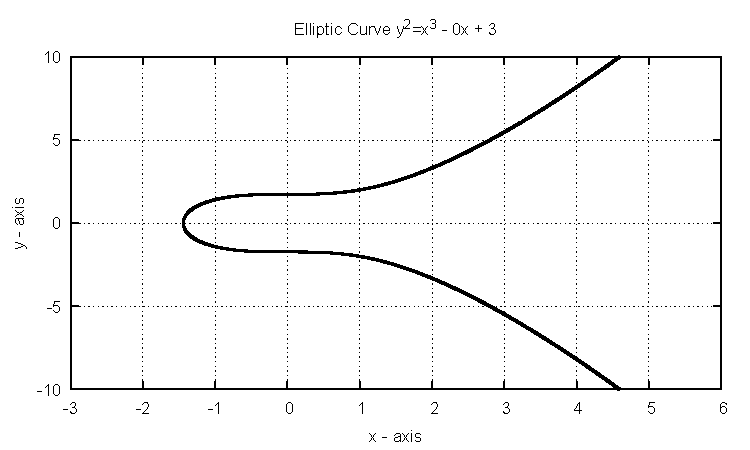
\includegraphics{../Images/ecc_plot/5}
  \end{minipage}
  \begin{minipage}{0.3\textwidth} \centering
    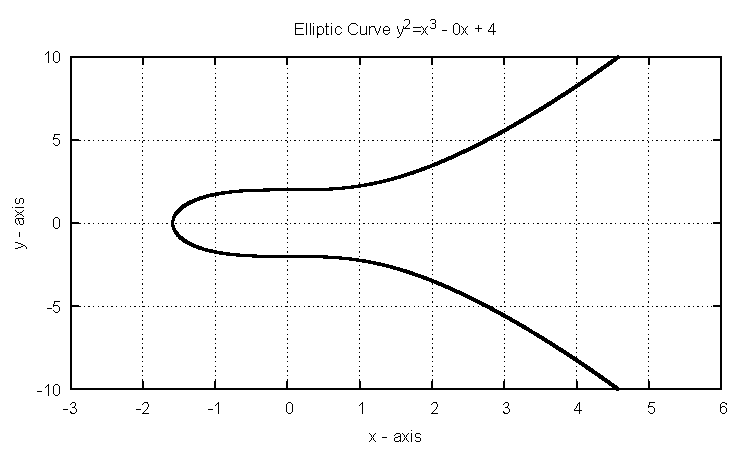
\includegraphics{../Images/ecc_plot/6}
  \end{minipage}
\end{figure}

\begin{figure}[!htbp]

  \begin{minipage}{0.3\textwidth} \centering
    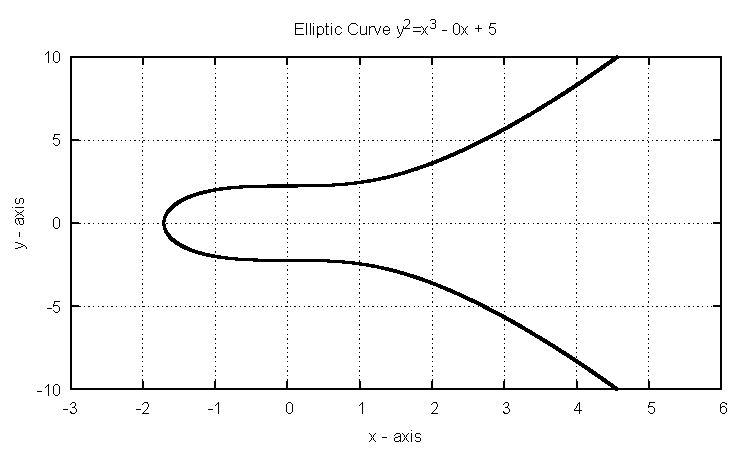
\includegraphics{../Images/ecc_plot/7}
  \end{minipage}
  \begin{minipage}{0.3\textwidth} \centering
    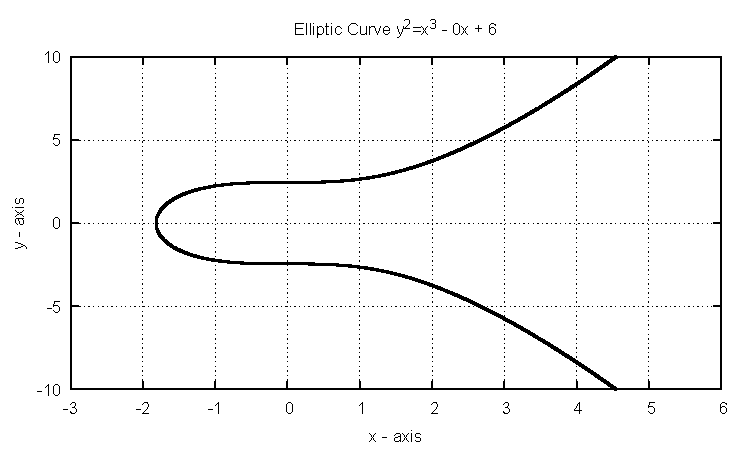
\includegraphics{../Images/ecc_plot/8}
  \end{minipage}
  \begin{minipage}{0.3\textwidth} \centering
    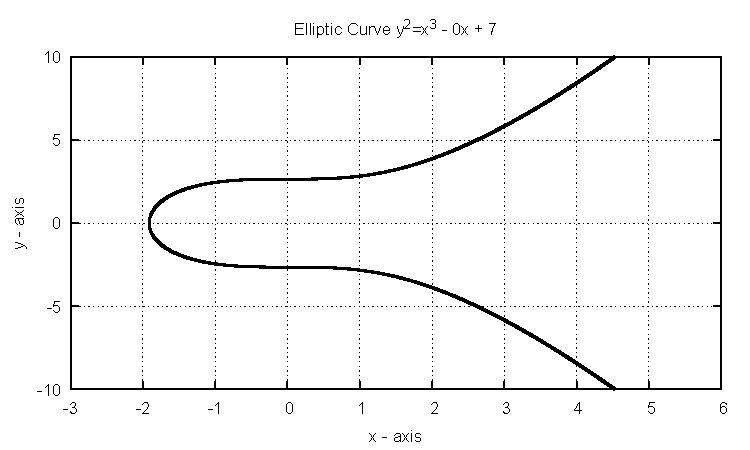
\includegraphics{../Images/ecc_plot/9}
  \end{minipage}
\end{figure}

\begin{figure}[!htbp]

  \begin{minipage}{0.3\textwidth} \centering
    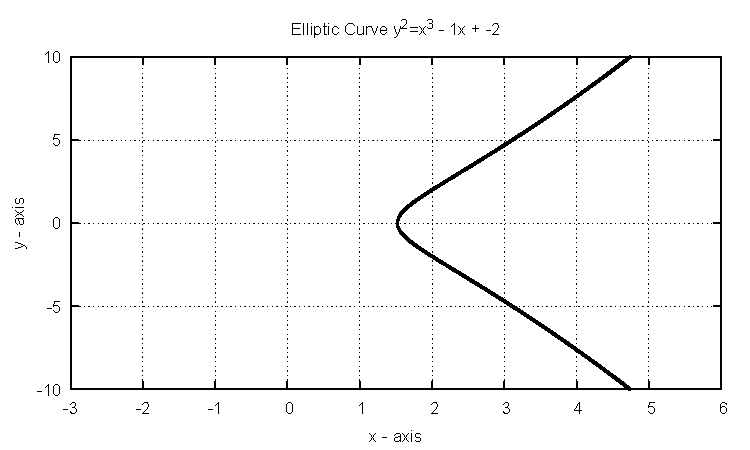
\includegraphics{../Images/ecc_plot/10}
  \end{minipage}
  \begin{minipage}{0.3\textwidth} \centering
    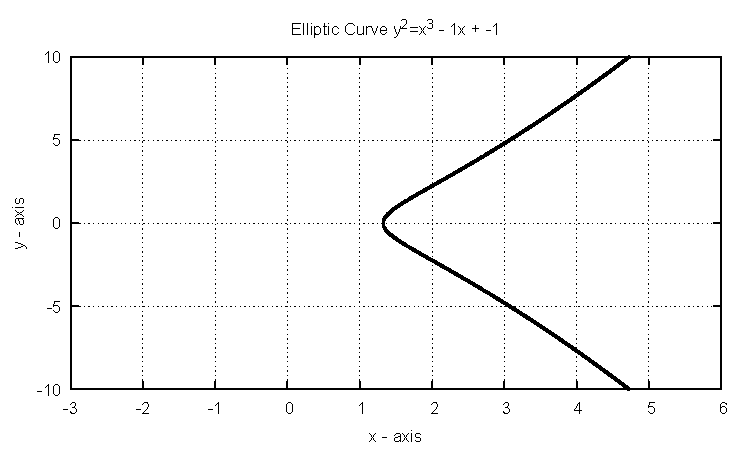
\includegraphics{../Images/ecc_plot/11}
  \end{minipage}
  \begin{minipage}{0.3\textwidth} \centering
    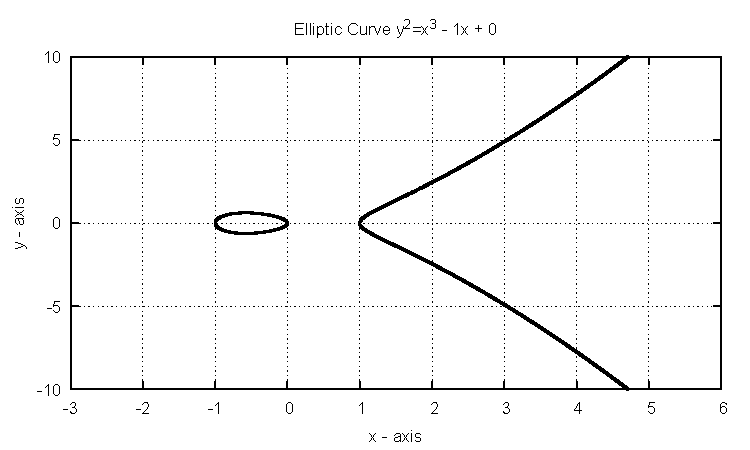
\includegraphics{../Images/ecc_plot/12}
  \end{minipage}
\end{figure}

\begin{figure}[!htbp]

  \begin{minipage}{0.3\textwidth} \centering
    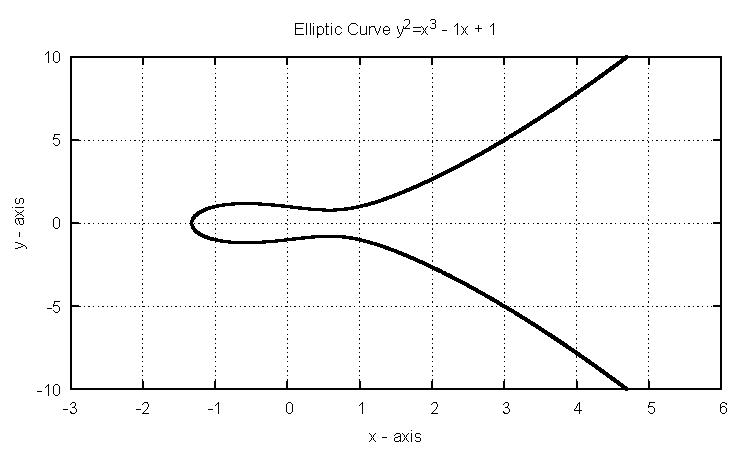
\includegraphics{../Images/ecc_plot/13}
  \end{minipage}
  \begin{minipage}{0.3\textwidth} \centering
    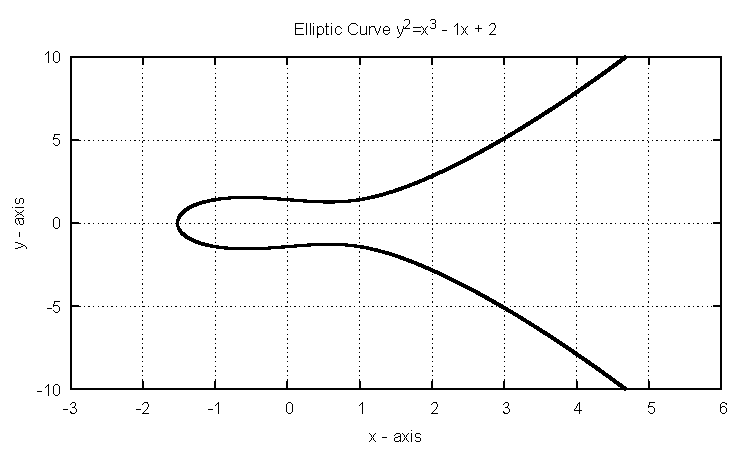
\includegraphics{../Images/ecc_plot/14}
  \end{minipage}
  \begin{minipage}{0.3\textwidth} \centering
    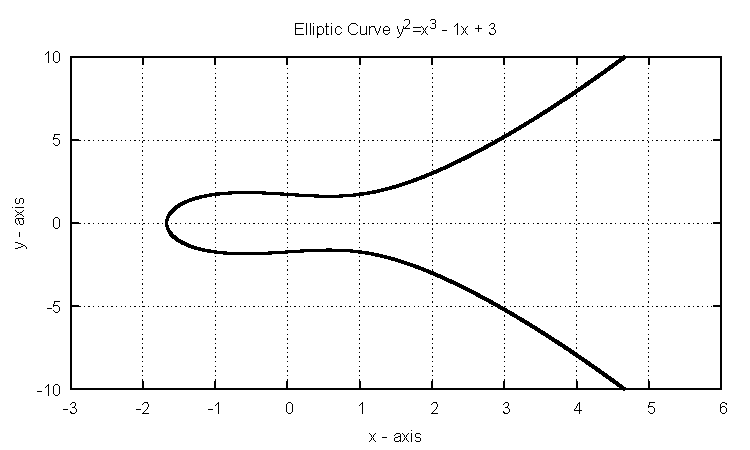
\includegraphics{../Images/ecc_plot/15}
  \end{minipage}
\end{figure}

\begin{figure}[!htbp]

  \begin{minipage}{0.3\textwidth} \centering
    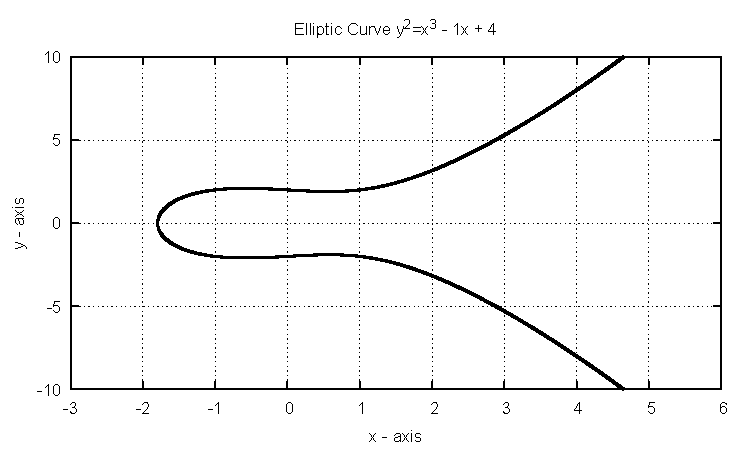
\includegraphics{../Images/ecc_plot/16}
  \end{minipage}
  \begin{minipage}{0.3\textwidth} \centering
    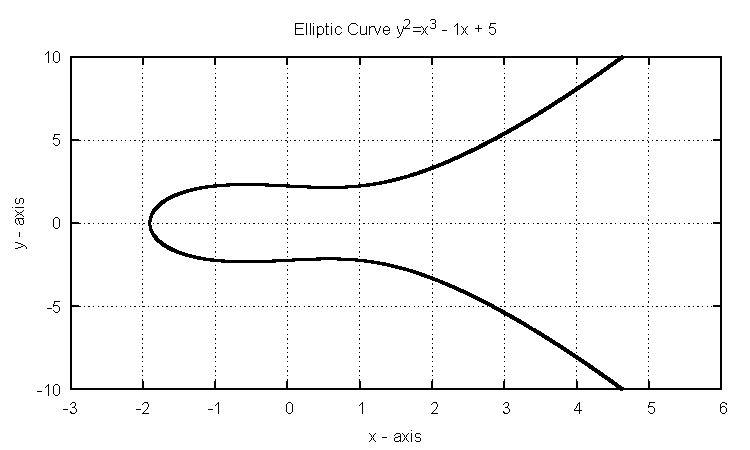
\includegraphics{../Images/ecc_plot/17}
  \end{minipage}
  \begin{minipage}{0.3\textwidth} \centering
    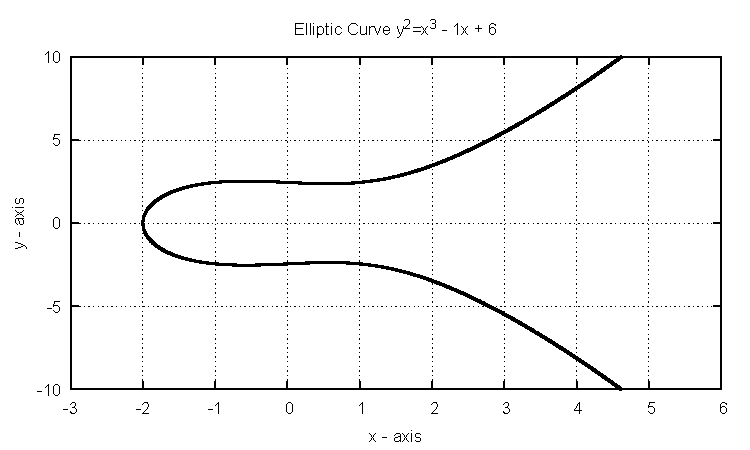
\includegraphics{../Images/ecc_plot/18}
  \end{minipage}
\end{figure}

\begin{figure}[!htbp]

  \begin{minipage}{0.3\textwidth} \centering
    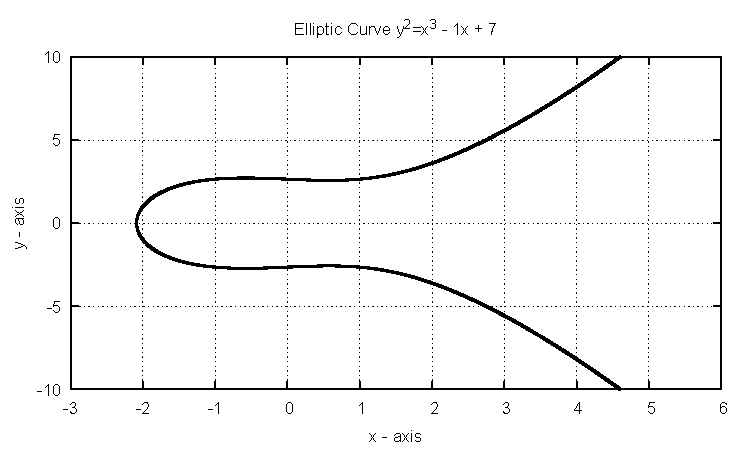
\includegraphics{../Images/ecc_plot/19}
  \end{minipage}
  \begin{minipage}{0.3\textwidth} \centering
    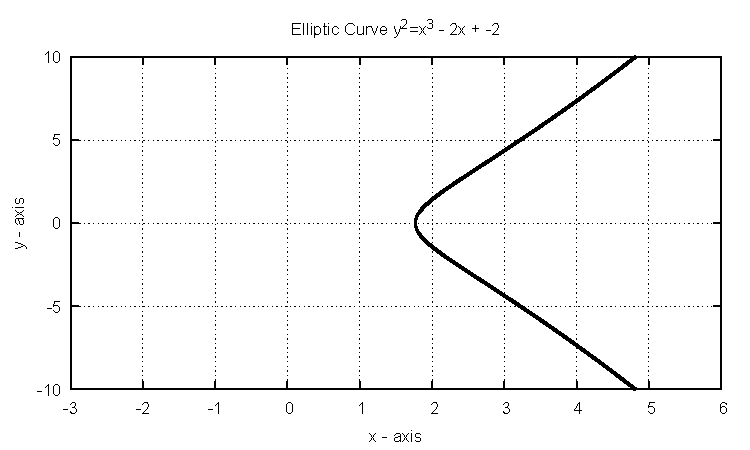
\includegraphics{../Images/ecc_plot/20}
  \end{minipage}
  \begin{minipage}{0.3\textwidth} \centering
    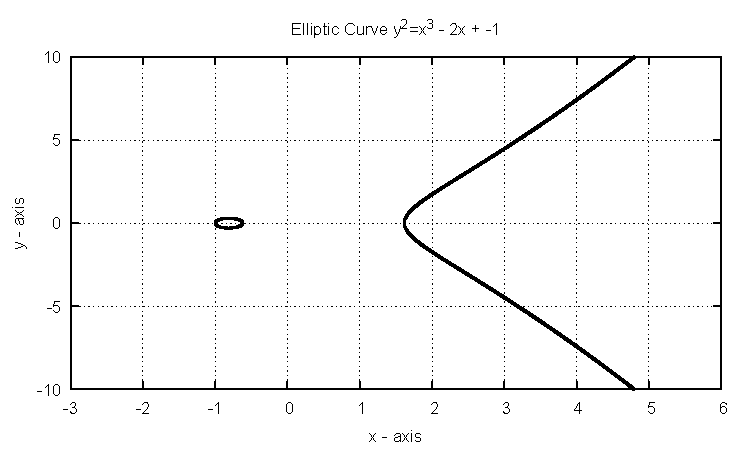
\includegraphics{../Images/ecc_plot/21}
  \end{minipage}
\end{figure}

\begin{figure}[!htbp]

  \begin{minipage}{0.3\textwidth} \centering
    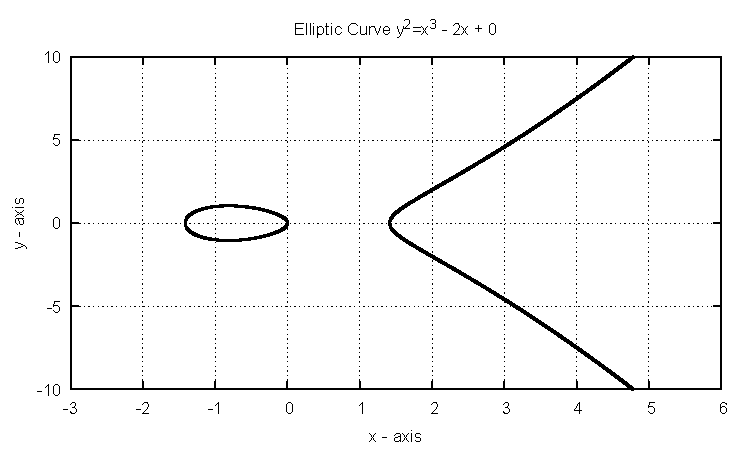
\includegraphics{../Images/ecc_plot/22}
  \end{minipage}
  \begin{minipage}{0.3\textwidth} \centering
    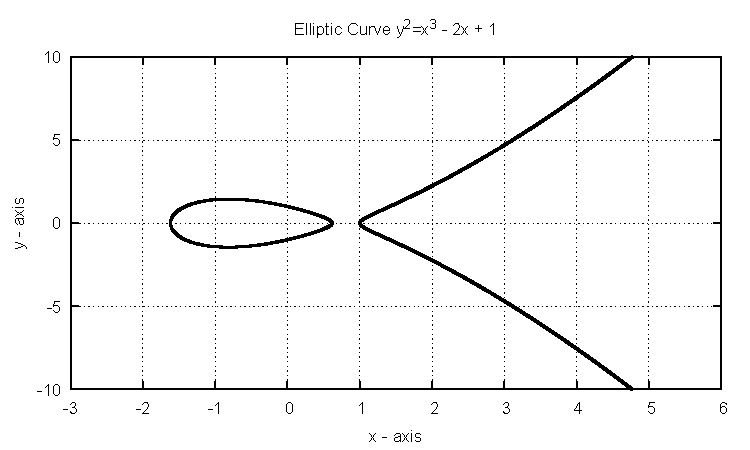
\includegraphics{../Images/ecc_plot/23}
  \end{minipage}
  \begin{minipage}{0.3\textwidth} \centering
    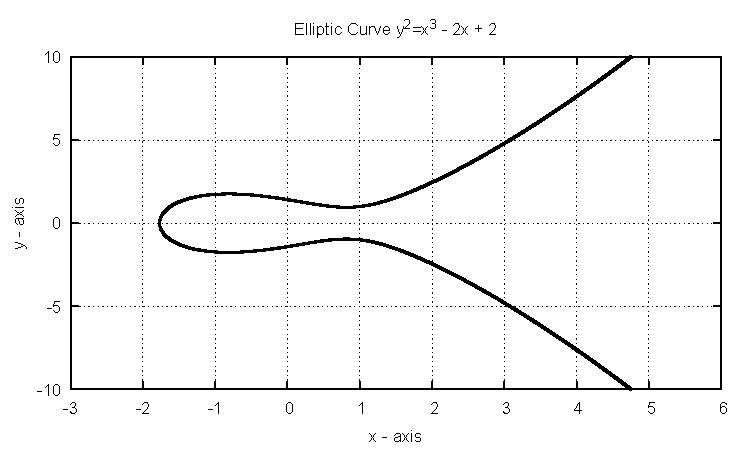
\includegraphics{../Images/ecc_plot/24}
  \end{minipage}
\end{figure}

\begin{figure}[!htbp]

  \begin{minipage}{0.3\textwidth} \centering
    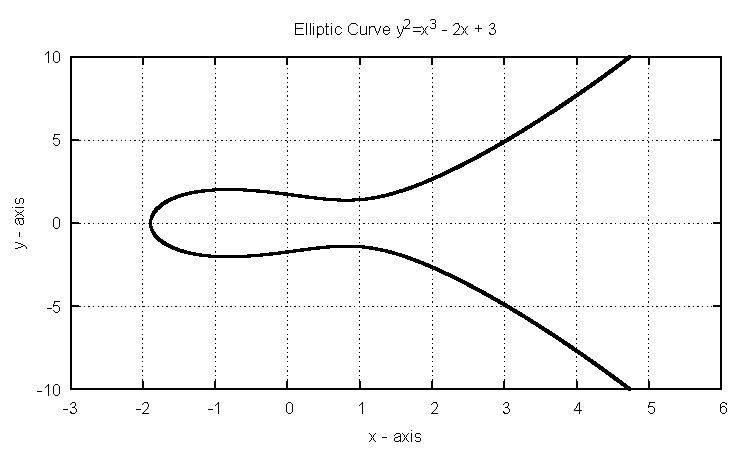
\includegraphics{../Images/ecc_plot/25}
  \end{minipage}
  \begin{minipage}{0.3\textwidth} \centering
    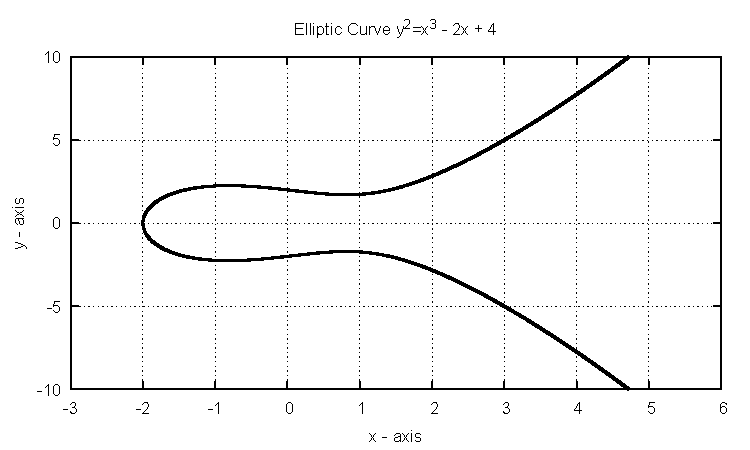
\includegraphics{../Images/ecc_plot/26}
  \end{minipage}
  \begin{minipage}{0.3\textwidth} \centering
    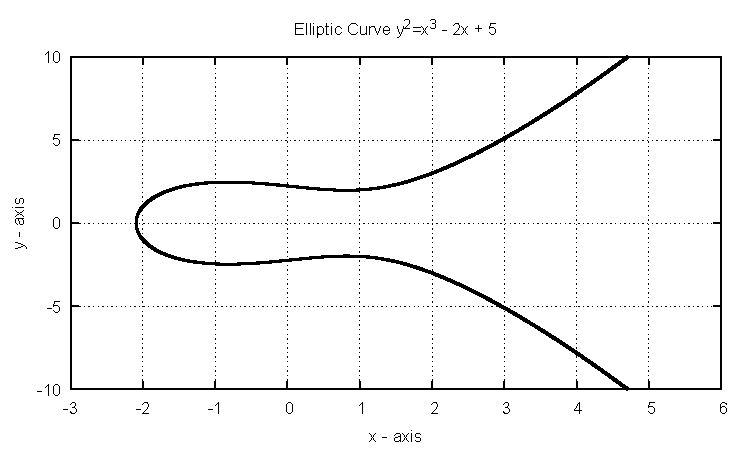
\includegraphics{../Images/ecc_plot/27}
  \end{minipage}
\end{figure}

\begin{figure}[!htbp]

  \begin{minipage}{0.3\textwidth} \centering
    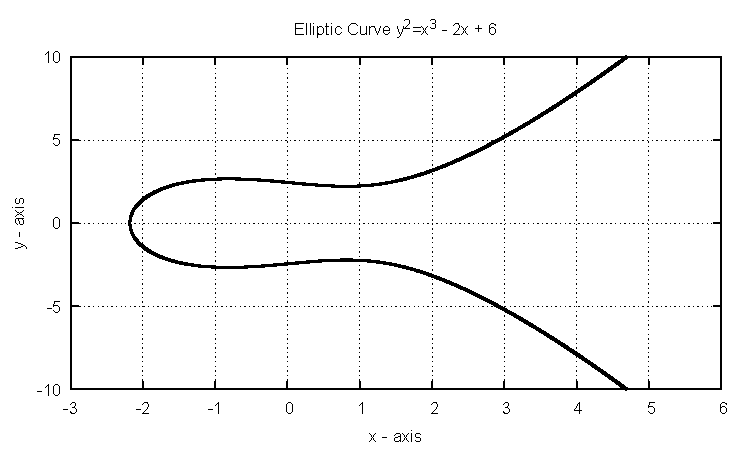
\includegraphics{../Images/ecc_plot/28}
  \end{minipage}
  \begin{minipage}{0.3\textwidth} \centering
    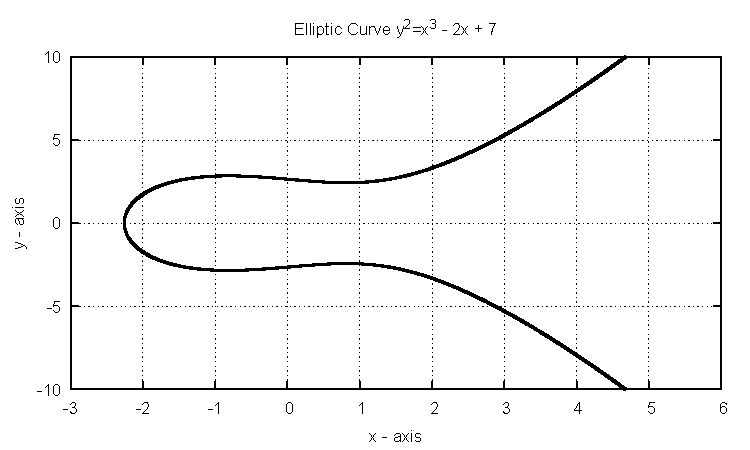
\includegraphics{../Images/ecc_plot/29}
  \end{minipage}
  \begin{minipage}{0.3\textwidth} \centering
    \includegraphics{../Images/ecc_plot/30}
  \end{minipage}
\end{figure}



%\begin{equation}
%    dS = \mu S dt + \sigma S dW
%\end{equation}
%
%where:
%\begin{itemize}
%    \item \( \mu \) is the drift rate of the stock.
%    \item \( \sigma \) is the volatility of the stock.
%    \item \( W \) is a Wiener process or Brownian motion.
%\end{itemize}
%
%\defn{Call and Put Options}{
%    \begin{itemize}
%        \item \textbf{Call Option:} Gives the holder the right (but not the obligation) to buy an asset at a predefined date and price (strike price).
%        \item \textbf{Put Option:} Gives the holder the right (but not the obligation) to sell an asset at a predefined date and price (strike price).
%    \end{itemize}
%}
%
%Under the black and scholes assumptions we the PDE of the price of an European Call :
%
%\thmp{Black and Scholes PDE }{
%\begin{equation}
%    \frac{\partial C}{\partial t} + r S \frac{\partial C}{\partial S} + \frac{1}{2} \sigma^2 S^2 \frac{\partial^2 C}{\partial S^2} = r C
%\end{equation}
%}{
%Using Ito's Lemma we get : 
%\begin{equation}
%    dC = \frac{\partial C}{\partial t} dt + \frac{\partial C}{\partial S} dS + \frac{1}{2} \frac{\partial^2 C}{\partial S^2} \sigma^2 S^2 dt
%\end{equation}
%
%Substituting \( dS \) into the equation, we get:
%
%\begin{equation}
%    dC = \left( \frac{\partial C}{\partial t} + \frac{\partial C}{\partial S} \mu S + \frac{1}{2} \frac{\partial^2 C}{\partial S^2} \sigma^2 S^2 \right) dt + \frac{\partial C}{\partial S} \sigma S dW
%\end{equation}
%
%This can be rearranged to:
%
%\begin{equation}
%    dC = \left( \frac{\partial C}{\partial t} + \frac{\partial C}{\partial S} \mu S + \frac{1}{2} \frac{\partial^2 C}{\partial S^2} \sigma^2 S^2 \right) dt + \frac{\partial C}{\partial S} \sigma S dW
%\end{equation}
%
%We form a risk-free portfolio by holding a position in the stock and an option. The change in the value of the portfolio is:
%
%\begin{equation}
%    \Pi = -C + \Delta S
%\end{equation}
%
%The change in the portfolio value is:
%
%\begin{equation}
%    d\Pi = -dC + \Delta dS
%\end{equation}
%
%Substituting \( dC \) and \( dS \), and choosing \( \Delta = \frac{\partial C}{\partial S} \), we get:
%
%\begin{equation}
%    d\Pi = -\left( \frac{\partial C}{\partial t} + \frac{1}{2} \frac{\partial^2 C}{\partial S^2} \sigma^2 S^2 \right) dt
%\end{equation}
%
%For the portfolio to be risk-free, \( d\Pi \) must earn the risk-free rate \( r \):
%
%\begin{equation}
%    -\left( \frac{\partial C}{\partial t} + \frac{1}{2} \frac{\partial^2 C}{\partial S^2} \sigma^2 S^2 \right) = r \left( -C + \frac{\partial C}{\partial S} S \right)
%\end{equation}
%
%Simplifying, we get the Black-Scholes partial differential equation:
%\begin{equation*}
%    \frac{\partial C}{\partial t} + r S \frac{\partial C}{\partial S} + \frac{1}{2} \sigma^2 S^2 \frac{\partial^2 C}{\partial S^2} = r C
%\end{equation*}
%
%}
%
%
%
%\section{Solution to the Black-Scholes Equation for Call Options}
%
%To solve the Black-Scholes equation, we apply the boundary condition for a European call option:
%
%\begin{equation}
%    C(S, T) = \max(S_T - K, 0)
%\end{equation}
%
%where \( K \) is the strike price and \( T \) is the time to expiration.
%
%Using the method of transforming variables, we obtain the solution for a call option:
%
%\thmp{Black and Scholes formulas}{
%The price of a call under black and scholes model is : 
%
%\begin{equation}
%    C(S, t) = S \Phi(d_1) - K e^{-r(T-t)} \Phi(d_2)
%\end{equation}
%
%where:
%\begin{align}
%    d_1 &= \frac{\ln\left(\frac{S}{K}\right) + \left(r + \frac{\sigma^2}{2}\right)(T-t)}{\sigma \sqrt{T-t}} \\
%    d_2 &= d_1 - \sigma \sqrt{T-t}
%\end{align}
%
%and \( \Phi \) is the cumulative distribution function of the standard normal distribution.
%
%}{
%Left exercise for reader. 
%}
%
%
%\section{Solution to the Black-Scholes Equation for Put Options}
%
%Similarly, for a European put option, the boundary condition is:
%
%\begin{equation}
%    P(S, T) = \max(K - S_T, 0)
%\end{equation}
%
%The solution for a put option is given by:
%
%\begin{equation}
%    P(S, t) = K e^{-r(T-t)} \Phi(-d_2) - S \Phi(-d_1)
%\end{equation}
%
%\section{Greeks in the Black-Scholes Model}
%
%The Greeks are sensitivities of the option price to various factors:
%
%\subsection{Delta}
%
%Delta measures the sensitivity of the option price to changes in the underlying asset price:
%
%\begin{equation}
%    \Delta_C = \frac{\partial C}{\partial S} = \Phi(d_1)
%\end{equation}
%
%\begin{equation}
%    \Delta_P = \frac{\partial P}{\partial S} = \Phi(d_1) - 1
%\end{equation}
%
%\subsection{Gamma}
%
%Gamma measures the sensitivity of delta to changes in the underlying asset price:
%
%\begin{equation}
%    \Gamma = \frac{\partial^2 C}{\partial S^2} = \frac{\Phi'(d_1)}{S \sigma \sqrt{T - t}}
%\end{equation}
%
%\subsection{Theta}
%
%Theta measures the sensitivity of the option price to the passage of time:
%
%\begin{equation}
%    \Theta_C = -\frac{S \Phi'(d_1) \sigma}{2 \sqrt{T - t}} - r K e^{-r(T - t)} \Phi(d_2)
%\end{equation}
%
%\begin{equation}
%    \Theta_P = -\frac{S \Phi'(d_1) \sigma}{2 \sqrt{T - t}} + r K e^{-r(T - t)} \Phi(-d_2)
%\end{equation}
%
%\subsection{Vega}
%
%Vega measures the sensitivity of the option price to changes in volatility:
%
%\begin{equation}
%    \nu = \frac{\partial C}{\partial \sigma} = \frac{\partial P}{\partial \sigma} = S \sqrt{T - t} \Phi'(d_1)
%\end{equation}
%
%\subsection{Rho}
%
%Rho measures the sensitivity of the option price to changes in the risk-free interest rate:
%
%\begin{equation}
%    \rho_C = K (T - t) e^{-r(T - t)} \Phi(d_2)
%\end{equation}
%
%\begin{equation}
%    \rho_P = -K (T - t) e^{-r(T - t)} \Phi(-d_2)
%\end{equation}
%
%
%\section{Numerical Examples}
%
%\exm{Call Option Pricing}{
%    Consider a European call option with \( S = 100 \), \( K = 100 \), \( r = 0.05 \), \( \sigma = 0.2 \), and \( T = 1 \) year. Using the Black-Scholes formula, we calculate the call option price.
%}
%
%
%\section{Conclusion}
%
%%\begin{figure}{2.9in}
%%%\resizebox{2.5in}{!}{% GNUPLOT: LaTeX picture with Postscript
\begingroup
  \makeatletter
  \providecommand\color[2][]{%
    \GenericError{(gnuplot) \space\space\space\@spaces}{%
      Package color not loaded in conjunction with
      terminal option `colourtext'%
    }{See the gnuplot documentation for explanation.%
    }{Either use 'blacktext' in gnuplot or load the package
      color.sty in LaTeX.}%
    \renewcommand\color[2][]{}%
  }%
  \providecommand\includegraphics[2][]{%
    \GenericError{(gnuplot) \space\space\space\@spaces}{%
      Package graphicx or graphics not loaded%
    }{See the gnuplot documentation for explanation.%
    }{The gnuplot epslatex terminal needs graphicx.sty or graphics.sty.}%
    \renewcommand\includegraphics[2][]{}%
  }%
  \providecommand\rotatebox[2]{#2}%
  \@ifundefined{ifGPcolor}{%
    \newif\ifGPcolor
    \GPcolorfalse
  }{}%
  \@ifundefined{ifGPblacktext}{%
    \newif\ifGPblacktext
    \GPblacktexttrue
  }{}%
  % define a \g@addto@macro without @ in the name:
  \let\gplgaddtomacro\g@addto@macro
  % define empty templates for all commands taking text:
  \gdef\gplbacktext{}%
  \gdef\gplfronttext{}%
  \makeatother
  \ifGPblacktext
    % no textcolor at all
    \def\colorrgb#1{}%
    \def\colorgray#1{}%
  \else
    % gray or color?
    \ifGPcolor
      \def\colorrgb#1{\color[rgb]{#1}}%
      \def\colorgray#1{\color[gray]{#1}}%
      \expandafter\def\csname LTw\endcsname{\color{white}}%
      \expandafter\def\csname LTb\endcsname{\color{black}}%
      \expandafter\def\csname LTa\endcsname{\color{black}}%
      \expandafter\def\csname LT0\endcsname{\color[rgb]{1,0,0}}%
      \expandafter\def\csname LT1\endcsname{\color[rgb]{0,1,0}}%
      \expandafter\def\csname LT2\endcsname{\color[rgb]{0,0,1}}%
      \expandafter\def\csname LT3\endcsname{\color[rgb]{1,0,1}}%
      \expandafter\def\csname LT4\endcsname{\color[rgb]{0,1,1}}%
      \expandafter\def\csname LT5\endcsname{\color[rgb]{1,1,0}}%
      \expandafter\def\csname LT6\endcsname{\color[rgb]{0,0,0}}%
      \expandafter\def\csname LT7\endcsname{\color[rgb]{1,0.3,0}}%
      \expandafter\def\csname LT8\endcsname{\color[rgb]{0.5,0.5,0.5}}%
    \else
      % gray
      \def\colorrgb#1{\color{black}}%
      \def\colorgray#1{\color[gray]{#1}}%
      \expandafter\def\csname LTw\endcsname{\color{white}}%
      \expandafter\def\csname LTb\endcsname{\color{black}}%
      \expandafter\def\csname LTa\endcsname{\color{black}}%
      \expandafter\def\csname LT0\endcsname{\color{black}}%
      \expandafter\def\csname LT1\endcsname{\color{black}}%
      \expandafter\def\csname LT2\endcsname{\color{black}}%
      \expandafter\def\csname LT3\endcsname{\color{black}}%
      \expandafter\def\csname LT4\endcsname{\color{black}}%
      \expandafter\def\csname LT5\endcsname{\color{black}}%
      \expandafter\def\csname LT6\endcsname{\color{black}}%
      \expandafter\def\csname LT7\endcsname{\color{black}}%
      \expandafter\def\csname LT8\endcsname{\color{black}}%
    \fi
  \fi
  \setlength{\unitlength}{0.0500bp}%
  \begin{picture}(7200.00,5040.00)%
    \gplgaddtomacro\gplbacktext{%
      \csname LTb\endcsname%
      \put(726,440){\makebox(0,0)[r]{\strut{}-0.4}}%
      \put(726,1003){\makebox(0,0)[r]{\strut{}-0.2}}%
      \put(726,1565){\makebox(0,0)[r]{\strut{} 0}}%
      \put(726,2128){\makebox(0,0)[r]{\strut{} 0.2}}%
      \put(726,2691){\makebox(0,0)[r]{\strut{} 0.4}}%
      \put(726,3254){\makebox(0,0)[r]{\strut{} 0.6}}%
      \put(726,3816){\makebox(0,0)[r]{\strut{} 0.8}}%
      \put(726,4379){\makebox(0,0)[r]{\strut{} 1}}%
      \put(858,220){\makebox(0,0){\strut{} 0}}%
      \put(1651,220){\makebox(0,0){\strut{} 2}}%
      \put(2443,220){\makebox(0,0){\strut{} 4}}%
      \put(3236,220){\makebox(0,0){\strut{} 6}}%
      \put(4029,220){\makebox(0,0){\strut{} 8}}%
      \put(4821,220){\makebox(0,0){\strut{} 10}}%
      \put(5614,220){\makebox(0,0){\strut{} 12}}%
      \put(6407,220){\makebox(0,0){\strut{} 14}}%
      \put(3830,4709){\makebox(0,0){\strut{}\Large Illustrating L’H\^opital’s Rule: $\frac{\sin(x)}{x}$}}%
      \put(4128,3394){\makebox(0,0)[l]{\strut{}\Large$\displaystyle \lim_{x\Longrightarrow0}\frac{\sin(x)}{x}=1$}}%
    }%
    \gplgaddtomacro\gplfronttext{%
    }%
    \gplbacktext
    \put(0,0){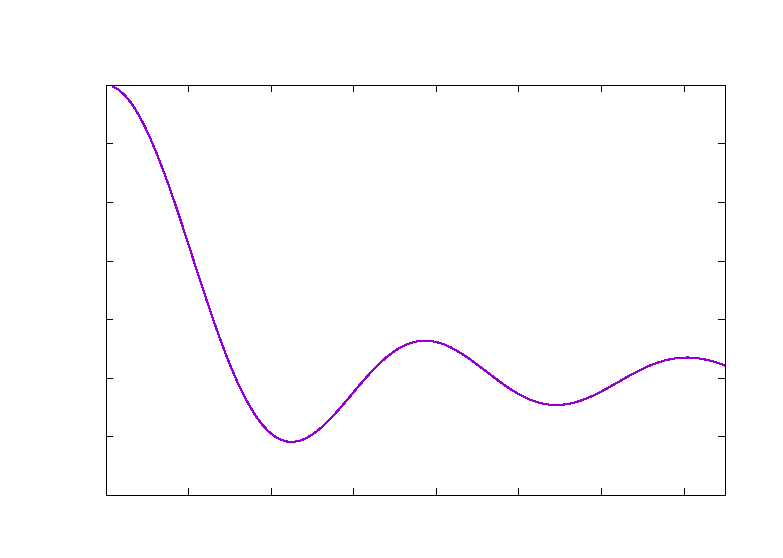
\includegraphics{r4}}%
    \gplfronttext
  \end{picture}%
\endgroup
}
%%%\scalebox{.5}{% GNUPLOT: LaTeX picture with Postscript
\begingroup
  \makeatletter
  \providecommand\color[2][]{%
    \GenericError{(gnuplot) \space\space\space\@spaces}{%
      Package color not loaded in conjunction with
      terminal option `colourtext'%
    }{See the gnuplot documentation for explanation.%
    }{Either use 'blacktext' in gnuplot or load the package
      color.sty in LaTeX.}%
    \renewcommand\color[2][]{}%
  }%
  \providecommand\includegraphics[2][]{%
    \GenericError{(gnuplot) \space\space\space\@spaces}{%
      Package graphicx or graphics not loaded%
    }{See the gnuplot documentation for explanation.%
    }{The gnuplot epslatex terminal needs graphicx.sty or graphics.sty.}%
    \renewcommand\includegraphics[2][]{}%
  }%
  \providecommand\rotatebox[2]{#2}%
  \@ifundefined{ifGPcolor}{%
    \newif\ifGPcolor
    \GPcolorfalse
  }{}%
  \@ifundefined{ifGPblacktext}{%
    \newif\ifGPblacktext
    \GPblacktexttrue
  }{}%
  % define a \g@addto@macro without @ in the name:
  \let\gplgaddtomacro\g@addto@macro
  % define empty templates for all commands taking text:
  \gdef\gplbacktext{}%
  \gdef\gplfronttext{}%
  \makeatother
  \ifGPblacktext
    % no textcolor at all
    \def\colorrgb#1{}%
    \def\colorgray#1{}%
  \else
    % gray or color?
    \ifGPcolor
      \def\colorrgb#1{\color[rgb]{#1}}%
      \def\colorgray#1{\color[gray]{#1}}%
      \expandafter\def\csname LTw\endcsname{\color{white}}%
      \expandafter\def\csname LTb\endcsname{\color{black}}%
      \expandafter\def\csname LTa\endcsname{\color{black}}%
      \expandafter\def\csname LT0\endcsname{\color[rgb]{1,0,0}}%
      \expandafter\def\csname LT1\endcsname{\color[rgb]{0,1,0}}%
      \expandafter\def\csname LT2\endcsname{\color[rgb]{0,0,1}}%
      \expandafter\def\csname LT3\endcsname{\color[rgb]{1,0,1}}%
      \expandafter\def\csname LT4\endcsname{\color[rgb]{0,1,1}}%
      \expandafter\def\csname LT5\endcsname{\color[rgb]{1,1,0}}%
      \expandafter\def\csname LT6\endcsname{\color[rgb]{0,0,0}}%
      \expandafter\def\csname LT7\endcsname{\color[rgb]{1,0.3,0}}%
      \expandafter\def\csname LT8\endcsname{\color[rgb]{0.5,0.5,0.5}}%
    \else
      % gray
      \def\colorrgb#1{\color{black}}%
      \def\colorgray#1{\color[gray]{#1}}%
      \expandafter\def\csname LTw\endcsname{\color{white}}%
      \expandafter\def\csname LTb\endcsname{\color{black}}%
      \expandafter\def\csname LTa\endcsname{\color{black}}%
      \expandafter\def\csname LT0\endcsname{\color{black}}%
      \expandafter\def\csname LT1\endcsname{\color{black}}%
      \expandafter\def\csname LT2\endcsname{\color{black}}%
      \expandafter\def\csname LT3\endcsname{\color{black}}%
      \expandafter\def\csname LT4\endcsname{\color{black}}%
      \expandafter\def\csname LT5\endcsname{\color{black}}%
      \expandafter\def\csname LT6\endcsname{\color{black}}%
      \expandafter\def\csname LT7\endcsname{\color{black}}%
      \expandafter\def\csname LT8\endcsname{\color{black}}%
    \fi
  \fi
  \setlength{\unitlength}{0.0500bp}%
  \begin{picture}(7200.00,5040.00)%
    \gplgaddtomacro\gplbacktext{%
      \csname LTb\endcsname%
      \put(726,440){\makebox(0,0)[r]{\strut{}-0.4}}%
      \put(726,1003){\makebox(0,0)[r]{\strut{}-0.2}}%
      \put(726,1565){\makebox(0,0)[r]{\strut{} 0}}%
      \put(726,2128){\makebox(0,0)[r]{\strut{} 0.2}}%
      \put(726,2691){\makebox(0,0)[r]{\strut{} 0.4}}%
      \put(726,3254){\makebox(0,0)[r]{\strut{} 0.6}}%
      \put(726,3816){\makebox(0,0)[r]{\strut{} 0.8}}%
      \put(726,4379){\makebox(0,0)[r]{\strut{} 1}}%
      \put(858,220){\makebox(0,0){\strut{} 0}}%
      \put(1651,220){\makebox(0,0){\strut{} 2}}%
      \put(2443,220){\makebox(0,0){\strut{} 4}}%
      \put(3236,220){\makebox(0,0){\strut{} 6}}%
      \put(4029,220){\makebox(0,0){\strut{} 8}}%
      \put(4821,220){\makebox(0,0){\strut{} 10}}%
      \put(5614,220){\makebox(0,0){\strut{} 12}}%
      \put(6407,220){\makebox(0,0){\strut{} 14}}%
      \put(3830,4709){\makebox(0,0){\strut{}\Large Illustrating L’H\^opital’s Rule: $\frac{\sin(x)}{x}$}}%
      \put(4128,3394){\makebox(0,0)[l]{\strut{}\Large$\displaystyle \lim_{x\Longrightarrow0}\frac{\sin(x)}{x}=1$}}%
    }%
    \gplgaddtomacro\gplfronttext{%
    }%
    \gplbacktext
    \put(0,0){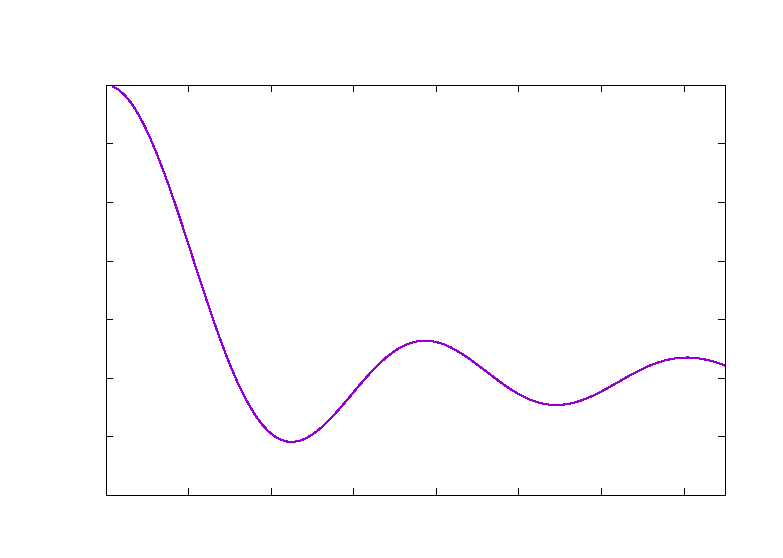
\includegraphics{r4}}%
    \gplfronttext
  \end{picture}%
\endgroup
}
%%\scalebox{.5}{% GNUPLOT: LaTeX picture with Postscript
\begingroup
  \makeatletter
  \providecommand\color[2][]{%
    \GenericError{(gnuplot) \space\space\space\@spaces}{%
      Package color not loaded in conjunction with
      terminal option `colourtext'%
    }{See the gnuplot documentation for explanation.%
    }{Either use 'blacktext' in gnuplot or load the package
      color.sty in LaTeX.}%
    \renewcommand\color[2][]{}%
  }%
  \providecommand\includegraphics[2][]{%
    \GenericError{(gnuplot) \space\space\space\@spaces}{%
      Package graphicx or graphics not loaded%
    }{See the gnuplot documentation for explanation.%
    }{The gnuplot epslatex terminal needs graphicx.sty or graphics.sty.}%
    \renewcommand\includegraphics[2][]{}%
  }%
  \providecommand\rotatebox[2]{#2}%
  \@ifundefined{ifGPcolor}{%
    \newif\ifGPcolor
    \GPcolorfalse
  }{}%
  \@ifundefined{ifGPblacktext}{%
    \newif\ifGPblacktext
    \GPblacktexttrue
  }{}%
  % define a \g@addto@macro without @ in the name:
  \let\gplgaddtomacro\g@addto@macro
  % define empty templates for all commands taking text:
  \gdef\gplbacktext{}%
  \gdef\gplfronttext{}%
  \makeatother
  \ifGPblacktext
    % no textcolor at all
    \def\colorrgb#1{}%
    \def\colorgray#1{}%
  \else
    % gray or color?
    \ifGPcolor
      \def\colorrgb#1{\color[rgb]{#1}}%
      \def\colorgray#1{\color[gray]{#1}}%
      \expandafter\def\csname LTw\endcsname{\color{white}}%
      \expandafter\def\csname LTb\endcsname{\color{black}}%
      \expandafter\def\csname LTa\endcsname{\color{black}}%
      \expandafter\def\csname LT0\endcsname{\color[rgb]{1,0,0}}%
      \expandafter\def\csname LT1\endcsname{\color[rgb]{0,1,0}}%
      \expandafter\def\csname LT2\endcsname{\color[rgb]{0,0,1}}%
      \expandafter\def\csname LT3\endcsname{\color[rgb]{1,0,1}}%
      \expandafter\def\csname LT4\endcsname{\color[rgb]{0,1,1}}%
      \expandafter\def\csname LT5\endcsname{\color[rgb]{1,1,0}}%
      \expandafter\def\csname LT6\endcsname{\color[rgb]{0,0,0}}%
      \expandafter\def\csname LT7\endcsname{\color[rgb]{1,0.3,0}}%
      \expandafter\def\csname LT8\endcsname{\color[rgb]{0.5,0.5,0.5}}%
    \else
      % gray
      \def\colorrgb#1{\color{black}}%
      \def\colorgray#1{\color[gray]{#1}}%
      \expandafter\def\csname LTw\endcsname{\color{white}}%
      \expandafter\def\csname LTb\endcsname{\color{black}}%
      \expandafter\def\csname LTa\endcsname{\color{black}}%
      \expandafter\def\csname LT0\endcsname{\color{black}}%
      \expandafter\def\csname LT1\endcsname{\color{black}}%
      \expandafter\def\csname LT2\endcsname{\color{black}}%
      \expandafter\def\csname LT3\endcsname{\color{black}}%
      \expandafter\def\csname LT4\endcsname{\color{black}}%
      \expandafter\def\csname LT5\endcsname{\color{black}}%
      \expandafter\def\csname LT6\endcsname{\color{black}}%
      \expandafter\def\csname LT7\endcsname{\color{black}}%
      \expandafter\def\csname LT8\endcsname{\color{black}}%
    \fi
  \fi
  \setlength{\unitlength}{0.0500bp}%
  \begin{picture}(7200.00,5040.00)%
    \gplgaddtomacro\gplbacktext{%
      \csname LTb\endcsname%
      \put(726,440){\makebox(0,0)[r]{\strut{}-0.4}}%
      \put(726,1003){\makebox(0,0)[r]{\strut{}-0.2}}%
      \put(726,1565){\makebox(0,0)[r]{\strut{} 0}}%
      \put(726,2128){\makebox(0,0)[r]{\strut{} 0.2}}%
      \put(726,2691){\makebox(0,0)[r]{\strut{} 0.4}}%
      \put(726,3254){\makebox(0,0)[r]{\strut{} 0.6}}%
      \put(726,3816){\makebox(0,0)[r]{\strut{} 0.8}}%
      \put(726,4379){\makebox(0,0)[r]{\strut{} 1}}%
      \put(858,220){\makebox(0,0){\strut{} 0}}%
      \put(1651,220){\makebox(0,0){\strut{} 2}}%
      \put(2443,220){\makebox(0,0){\strut{} 4}}%
      \put(3236,220){\makebox(0,0){\strut{} 6}}%
      \put(4029,220){\makebox(0,0){\strut{} 8}}%
      \put(4821,220){\makebox(0,0){\strut{} 10}}%
      \put(5614,220){\makebox(0,0){\strut{} 12}}%
      \put(6407,220){\makebox(0,0){\strut{} 14}}%
      \put(3830,4709){\makebox(0,0){\strut{}\Large Illustrating L’H\^opital’s Rule: $\frac{\sin(x)}{x}$}}%
      \put(4128,3394){\makebox(0,0)[l]{\strut{}\Large$\displaystyle \lim_{x\Longrightarrow0}\frac{\sin(x)}{x}=1$}}%
    }%
    \gplgaddtomacro\gplfronttext{%
    }%
    \gplbacktext
    \put(0,0){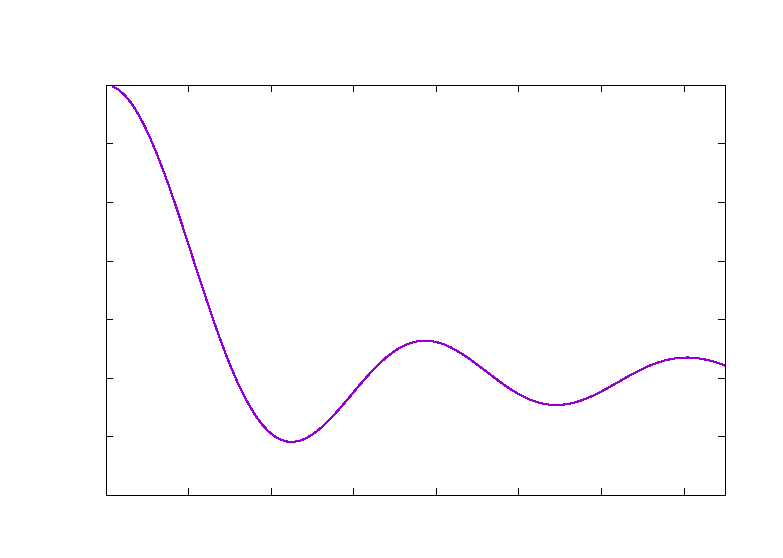
\includegraphics{r4}}%
    \gplfronttext
  \end{picture}%
\endgroup
}
%%%\scalebox{.5}{% GNUPLOT: LaTeX picture with Postscript
\begingroup
  \makeatletter
  \providecommand\color[2][]{%
    \GenericError{(gnuplot) \space\space\space\@spaces}{%
      Package color not loaded in conjunction with
      terminal option `colourtext'%
    }{See the gnuplot documentation for explanation.%
    }{Either use 'blacktext' in gnuplot or load the package
      color.sty in LaTeX.}%
    \renewcommand\color[2][]{}%
  }%
  \providecommand\includegraphics[2][]{%
    \GenericError{(gnuplot) \space\space\space\@spaces}{%
      Package graphicx or graphics not loaded%
    }{See the gnuplot documentation for explanation.%
    }{The gnuplot epslatex terminal needs graphicx.sty or graphics.sty.}%
    \renewcommand\includegraphics[2][]{}%
  }%
  \providecommand\rotatebox[2]{#2}%
  \@ifundefined{ifGPcolor}{%
    \newif\ifGPcolor
    \GPcolorfalse
  }{}%
  \@ifundefined{ifGPblacktext}{%
    \newif\ifGPblacktext
    \GPblacktexttrue
  }{}%
  % define a \g@addto@macro without @ in the name:
  \let\gplgaddtomacro\g@addto@macro
  % define empty templates for all commands taking text:
  \gdef\gplbacktext{}%
  \gdef\gplfronttext{}%
  \makeatother
  \ifGPblacktext
    % no textcolor at all
    \def\colorrgb#1{}%
    \def\colorgray#1{}%
  \else
    % gray or color?
    \ifGPcolor
      \def\colorrgb#1{\color[rgb]{#1}}%
      \def\colorgray#1{\color[gray]{#1}}%
      \expandafter\def\csname LTw\endcsname{\color{white}}%
      \expandafter\def\csname LTb\endcsname{\color{black}}%
      \expandafter\def\csname LTa\endcsname{\color{black}}%
      \expandafter\def\csname LT0\endcsname{\color[rgb]{1,0,0}}%
      \expandafter\def\csname LT1\endcsname{\color[rgb]{0,1,0}}%
      \expandafter\def\csname LT2\endcsname{\color[rgb]{0,0,1}}%
      \expandafter\def\csname LT3\endcsname{\color[rgb]{1,0,1}}%
      \expandafter\def\csname LT4\endcsname{\color[rgb]{0,1,1}}%
      \expandafter\def\csname LT5\endcsname{\color[rgb]{1,1,0}}%
      \expandafter\def\csname LT6\endcsname{\color[rgb]{0,0,0}}%
      \expandafter\def\csname LT7\endcsname{\color[rgb]{1,0.3,0}}%
      \expandafter\def\csname LT8\endcsname{\color[rgb]{0.5,0.5,0.5}}%
    \else
      % gray
      \def\colorrgb#1{\color{black}}%
      \def\colorgray#1{\color[gray]{#1}}%
      \expandafter\def\csname LTw\endcsname{\color{white}}%
      \expandafter\def\csname LTb\endcsname{\color{black}}%
      \expandafter\def\csname LTa\endcsname{\color{black}}%
      \expandafter\def\csname LT0\endcsname{\color{black}}%
      \expandafter\def\csname LT1\endcsname{\color{black}}%
      \expandafter\def\csname LT2\endcsname{\color{black}}%
      \expandafter\def\csname LT3\endcsname{\color{black}}%
      \expandafter\def\csname LT4\endcsname{\color{black}}%
      \expandafter\def\csname LT5\endcsname{\color{black}}%
      \expandafter\def\csname LT6\endcsname{\color{black}}%
      \expandafter\def\csname LT7\endcsname{\color{black}}%
      \expandafter\def\csname LT8\endcsname{\color{black}}%
    \fi
  \fi
  \setlength{\unitlength}{0.0500bp}%
  \begin{picture}(7200.00,5040.00)%
    \gplgaddtomacro\gplbacktext{%
      \csname LTb\endcsname%
      \put(726,440){\makebox(0,0)[r]{\strut{}-0.4}}%
      \put(726,1003){\makebox(0,0)[r]{\strut{}-0.2}}%
      \put(726,1565){\makebox(0,0)[r]{\strut{} 0}}%
      \put(726,2128){\makebox(0,0)[r]{\strut{} 0.2}}%
      \put(726,2691){\makebox(0,0)[r]{\strut{} 0.4}}%
      \put(726,3254){\makebox(0,0)[r]{\strut{} 0.6}}%
      \put(726,3816){\makebox(0,0)[r]{\strut{} 0.8}}%
      \put(726,4379){\makebox(0,0)[r]{\strut{} 1}}%
      \put(858,220){\makebox(0,0){\strut{} 0}}%
      \put(1651,220){\makebox(0,0){\strut{} 2}}%
      \put(2443,220){\makebox(0,0){\strut{} 4}}%
      \put(3236,220){\makebox(0,0){\strut{} 6}}%
      \put(4029,220){\makebox(0,0){\strut{} 8}}%
      \put(4821,220){\makebox(0,0){\strut{} 10}}%
      \put(5614,220){\makebox(0,0){\strut{} 12}}%
      \put(6407,220){\makebox(0,0){\strut{} 14}}%
      \put(3830,4709){\makebox(0,0){\strut{}\Large Illustrating L’H\^opital’s Rule: $\frac{\sin(x)}{x}$}}%
      \put(4128,3394){\makebox(0,0)[l]{\strut{}\Large$\displaystyle \lim_{x\Longrightarrow0}\frac{\sin(x)}{x}=1$}}%
    }%
    \gplgaddtomacro\gplfronttext{%
    }%
    \gplbacktext
    \put(0,0){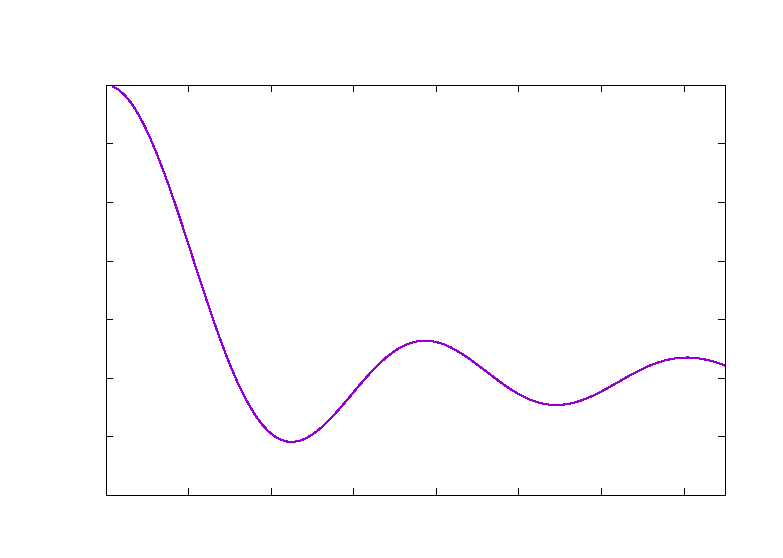
\includegraphics{r4}}%
    \gplfronttext
  \end{picture}%
\endgroup
}
%%%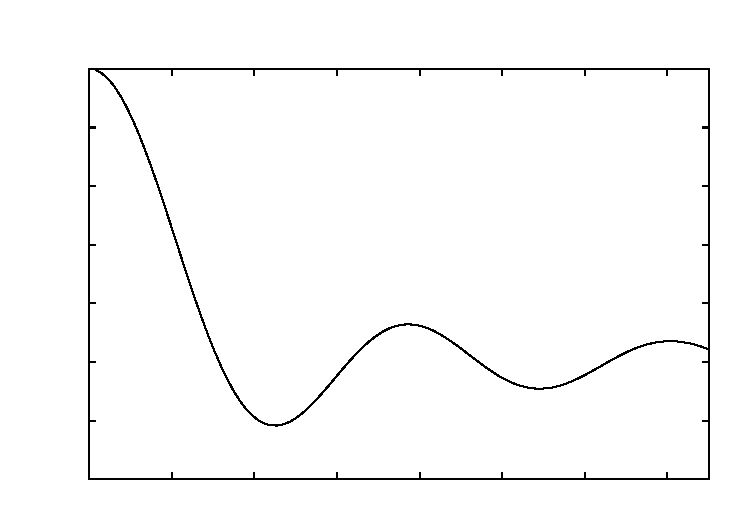
\includegraphics{../Images/ecc_plot/r4}
%%\end{figure}
%%
%%\begin{figure}{2.9in}
%%%\resizebox{2.5in}{!}{% GNUPLOT: LaTeX picture with Postscript
\begingroup
  \makeatletter
  \providecommand\color[2][]{%
    \GenericError{(gnuplot) \space\space\space\@spaces}{%
      Package color not loaded in conjunction with
      terminal option `colourtext'%
    }{See the gnuplot documentation for explanation.%
    }{Either use 'blacktext' in gnuplot or load the package
      color.sty in LaTeX.}%
    \renewcommand\color[2][]{}%
  }%
  \providecommand\includegraphics[2][]{%
    \GenericError{(gnuplot) \space\space\space\@spaces}{%
      Package graphicx or graphics not loaded%
    }{See the gnuplot documentation for explanation.%
    }{The gnuplot epslatex terminal needs graphicx.sty or graphics.sty.}%
    \renewcommand\includegraphics[2][]{}%
  }%
  \providecommand\rotatebox[2]{#2}%
  \@ifundefined{ifGPcolor}{%
    \newif\ifGPcolor
    \GPcolorfalse
  }{}%
  \@ifundefined{ifGPblacktext}{%
    \newif\ifGPblacktext
    \GPblacktexttrue
  }{}%
  % define a \g@addto@macro without @ in the name:
  \let\gplgaddtomacro\g@addto@macro
  % define empty templates for all commands taking text:
  \gdef\gplbacktext{}%
  \gdef\gplfronttext{}%
  \makeatother
  \ifGPblacktext
    % no textcolor at all
    \def\colorrgb#1{}%
    \def\colorgray#1{}%
  \else
    % gray or color?
    \ifGPcolor
      \def\colorrgb#1{\color[rgb]{#1}}%
      \def\colorgray#1{\color[gray]{#1}}%
      \expandafter\def\csname LTw\endcsname{\color{white}}%
      \expandafter\def\csname LTb\endcsname{\color{black}}%
      \expandafter\def\csname LTa\endcsname{\color{black}}%
      \expandafter\def\csname LT0\endcsname{\color[rgb]{1,0,0}}%
      \expandafter\def\csname LT1\endcsname{\color[rgb]{0,1,0}}%
      \expandafter\def\csname LT2\endcsname{\color[rgb]{0,0,1}}%
      \expandafter\def\csname LT3\endcsname{\color[rgb]{1,0,1}}%
      \expandafter\def\csname LT4\endcsname{\color[rgb]{0,1,1}}%
      \expandafter\def\csname LT5\endcsname{\color[rgb]{1,1,0}}%
      \expandafter\def\csname LT6\endcsname{\color[rgb]{0,0,0}}%
      \expandafter\def\csname LT7\endcsname{\color[rgb]{1,0.3,0}}%
      \expandafter\def\csname LT8\endcsname{\color[rgb]{0.5,0.5,0.5}}%
    \else
      % gray
      \def\colorrgb#1{\color{black}}%
      \def\colorgray#1{\color[gray]{#1}}%
      \expandafter\def\csname LTw\endcsname{\color{white}}%
      \expandafter\def\csname LTb\endcsname{\color{black}}%
      \expandafter\def\csname LTa\endcsname{\color{black}}%
      \expandafter\def\csname LT0\endcsname{\color{black}}%
      \expandafter\def\csname LT1\endcsname{\color{black}}%
      \expandafter\def\csname LT2\endcsname{\color{black}}%
      \expandafter\def\csname LT3\endcsname{\color{black}}%
      \expandafter\def\csname LT4\endcsname{\color{black}}%
      \expandafter\def\csname LT5\endcsname{\color{black}}%
      \expandafter\def\csname LT6\endcsname{\color{black}}%
      \expandafter\def\csname LT7\endcsname{\color{black}}%
      \expandafter\def\csname LT8\endcsname{\color{black}}%
    \fi
  \fi
  \setlength{\unitlength}{0.0500bp}%
  \begin{picture}(7200.00,5040.00)%
    \gplgaddtomacro\gplbacktext{%
      \csname LTb\endcsname%
      \put(726,440){\makebox(0,0)[r]{\strut{}-0.4}}%
      \put(726,1003){\makebox(0,0)[r]{\strut{}-0.2}}%
      \put(726,1565){\makebox(0,0)[r]{\strut{} 0}}%
      \put(726,2128){\makebox(0,0)[r]{\strut{} 0.2}}%
      \put(726,2691){\makebox(0,0)[r]{\strut{} 0.4}}%
      \put(726,3254){\makebox(0,0)[r]{\strut{} 0.6}}%
      \put(726,3816){\makebox(0,0)[r]{\strut{} 0.8}}%
      \put(726,4379){\makebox(0,0)[r]{\strut{} 1}}%
      \put(858,220){\makebox(0,0){\strut{} 0}}%
      \put(1651,220){\makebox(0,0){\strut{} 2}}%
      \put(2443,220){\makebox(0,0){\strut{} 4}}%
      \put(3236,220){\makebox(0,0){\strut{} 6}}%
      \put(4029,220){\makebox(0,0){\strut{} 8}}%
      \put(4821,220){\makebox(0,0){\strut{} 10}}%
      \put(5614,220){\makebox(0,0){\strut{} 12}}%
      \put(6407,220){\makebox(0,0){\strut{} 14}}%
      \put(3830,4709){\makebox(0,0){\strut{}\Large Illustrating L’H\^opital’s Rule: $\frac{\sin(x)}{x}$}}%
      \put(4128,3394){\makebox(0,0)[l]{\strut{}\Large$\displaystyle \lim_{x\Longrightarrow0}\frac{\sin(x)}{x}=1$}}%
    }%
    \gplgaddtomacro\gplfronttext{%
    }%
    \gplbacktext
    \put(0,0){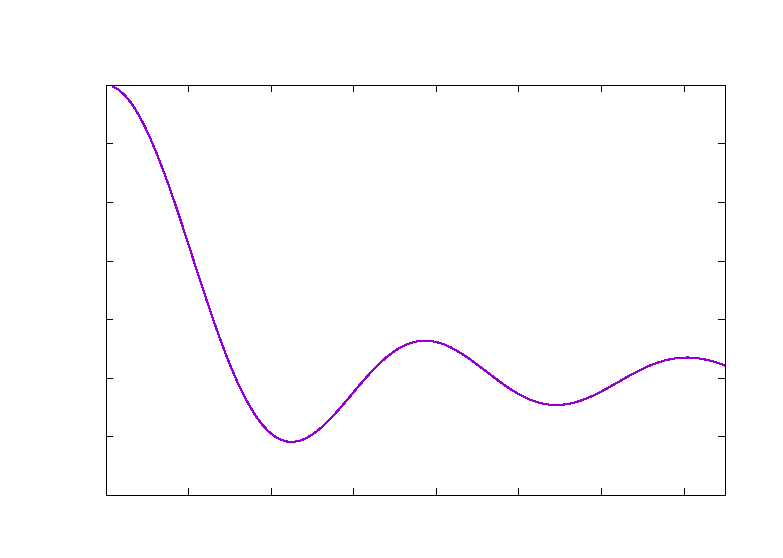
\includegraphics{r4}}%
    \gplfronttext
  \end{picture}%
\endgroup
}
%%%\scalebox{.5}{% GNUPLOT: LaTeX picture with Postscript
\begingroup
  \makeatletter
  \providecommand\color[2][]{%
    \GenericError{(gnuplot) \space\space\space\@spaces}{%
      Package color not loaded in conjunction with
      terminal option `colourtext'%
    }{See the gnuplot documentation for explanation.%
    }{Either use 'blacktext' in gnuplot or load the package
      color.sty in LaTeX.}%
    \renewcommand\color[2][]{}%
  }%
  \providecommand\includegraphics[2][]{%
    \GenericError{(gnuplot) \space\space\space\@spaces}{%
      Package graphicx or graphics not loaded%
    }{See the gnuplot documentation for explanation.%
    }{The gnuplot epslatex terminal needs graphicx.sty or graphics.sty.}%
    \renewcommand\includegraphics[2][]{}%
  }%
  \providecommand\rotatebox[2]{#2}%
  \@ifundefined{ifGPcolor}{%
    \newif\ifGPcolor
    \GPcolorfalse
  }{}%
  \@ifundefined{ifGPblacktext}{%
    \newif\ifGPblacktext
    \GPblacktexttrue
  }{}%
  % define a \g@addto@macro without @ in the name:
  \let\gplgaddtomacro\g@addto@macro
  % define empty templates for all commands taking text:
  \gdef\gplbacktext{}%
  \gdef\gplfronttext{}%
  \makeatother
  \ifGPblacktext
    % no textcolor at all
    \def\colorrgb#1{}%
    \def\colorgray#1{}%
  \else
    % gray or color?
    \ifGPcolor
      \def\colorrgb#1{\color[rgb]{#1}}%
      \def\colorgray#1{\color[gray]{#1}}%
      \expandafter\def\csname LTw\endcsname{\color{white}}%
      \expandafter\def\csname LTb\endcsname{\color{black}}%
      \expandafter\def\csname LTa\endcsname{\color{black}}%
      \expandafter\def\csname LT0\endcsname{\color[rgb]{1,0,0}}%
      \expandafter\def\csname LT1\endcsname{\color[rgb]{0,1,0}}%
      \expandafter\def\csname LT2\endcsname{\color[rgb]{0,0,1}}%
      \expandafter\def\csname LT3\endcsname{\color[rgb]{1,0,1}}%
      \expandafter\def\csname LT4\endcsname{\color[rgb]{0,1,1}}%
      \expandafter\def\csname LT5\endcsname{\color[rgb]{1,1,0}}%
      \expandafter\def\csname LT6\endcsname{\color[rgb]{0,0,0}}%
      \expandafter\def\csname LT7\endcsname{\color[rgb]{1,0.3,0}}%
      \expandafter\def\csname LT8\endcsname{\color[rgb]{0.5,0.5,0.5}}%
    \else
      % gray
      \def\colorrgb#1{\color{black}}%
      \def\colorgray#1{\color[gray]{#1}}%
      \expandafter\def\csname LTw\endcsname{\color{white}}%
      \expandafter\def\csname LTb\endcsname{\color{black}}%
      \expandafter\def\csname LTa\endcsname{\color{black}}%
      \expandafter\def\csname LT0\endcsname{\color{black}}%
      \expandafter\def\csname LT1\endcsname{\color{black}}%
      \expandafter\def\csname LT2\endcsname{\color{black}}%
      \expandafter\def\csname LT3\endcsname{\color{black}}%
      \expandafter\def\csname LT4\endcsname{\color{black}}%
      \expandafter\def\csname LT5\endcsname{\color{black}}%
      \expandafter\def\csname LT6\endcsname{\color{black}}%
      \expandafter\def\csname LT7\endcsname{\color{black}}%
      \expandafter\def\csname LT8\endcsname{\color{black}}%
    \fi
  \fi
  \setlength{\unitlength}{0.0500bp}%
  \begin{picture}(7200.00,5040.00)%
    \gplgaddtomacro\gplbacktext{%
      \csname LTb\endcsname%
      \put(726,440){\makebox(0,0)[r]{\strut{}-0.4}}%
      \put(726,1003){\makebox(0,0)[r]{\strut{}-0.2}}%
      \put(726,1565){\makebox(0,0)[r]{\strut{} 0}}%
      \put(726,2128){\makebox(0,0)[r]{\strut{} 0.2}}%
      \put(726,2691){\makebox(0,0)[r]{\strut{} 0.4}}%
      \put(726,3254){\makebox(0,0)[r]{\strut{} 0.6}}%
      \put(726,3816){\makebox(0,0)[r]{\strut{} 0.8}}%
      \put(726,4379){\makebox(0,0)[r]{\strut{} 1}}%
      \put(858,220){\makebox(0,0){\strut{} 0}}%
      \put(1651,220){\makebox(0,0){\strut{} 2}}%
      \put(2443,220){\makebox(0,0){\strut{} 4}}%
      \put(3236,220){\makebox(0,0){\strut{} 6}}%
      \put(4029,220){\makebox(0,0){\strut{} 8}}%
      \put(4821,220){\makebox(0,0){\strut{} 10}}%
      \put(5614,220){\makebox(0,0){\strut{} 12}}%
      \put(6407,220){\makebox(0,0){\strut{} 14}}%
      \put(3830,4709){\makebox(0,0){\strut{}\Large Illustrating L’H\^opital’s Rule: $\frac{\sin(x)}{x}$}}%
      \put(4128,3394){\makebox(0,0)[l]{\strut{}\Large$\displaystyle \lim_{x\Longrightarrow0}\frac{\sin(x)}{x}=1$}}%
    }%
    \gplgaddtomacro\gplfronttext{%
    }%
    \gplbacktext
    \put(0,0){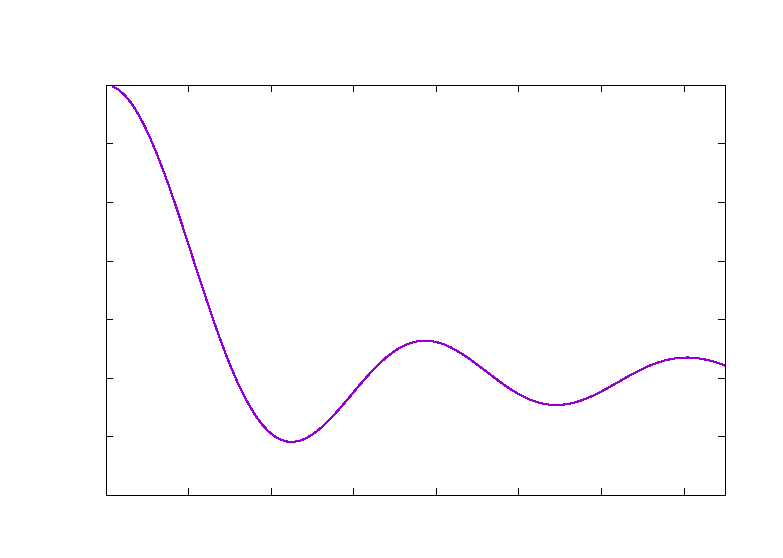
\includegraphics{r4}}%
    \gplfronttext
  \end{picture}%
\endgroup
}
%%\scalebox{.5}{\input{../Images/ecc_plot/ecc_2_3.tex}}
%%%\scalebox{.5}{% GNUPLOT: LaTeX picture with Postscript
\begingroup
  \makeatletter
  \providecommand\color[2][]{%
    \GenericError{(gnuplot) \space\space\space\@spaces}{%
      Package color not loaded in conjunction with
      terminal option `colourtext'%
    }{See the gnuplot documentation for explanation.%
    }{Either use 'blacktext' in gnuplot or load the package
      color.sty in LaTeX.}%
    \renewcommand\color[2][]{}%
  }%
  \providecommand\includegraphics[2][]{%
    \GenericError{(gnuplot) \space\space\space\@spaces}{%
      Package graphicx or graphics not loaded%
    }{See the gnuplot documentation for explanation.%
    }{The gnuplot epslatex terminal needs graphicx.sty or graphics.sty.}%
    \renewcommand\includegraphics[2][]{}%
  }%
  \providecommand\rotatebox[2]{#2}%
  \@ifundefined{ifGPcolor}{%
    \newif\ifGPcolor
    \GPcolorfalse
  }{}%
  \@ifundefined{ifGPblacktext}{%
    \newif\ifGPblacktext
    \GPblacktexttrue
  }{}%
  % define a \g@addto@macro without @ in the name:
  \let\gplgaddtomacro\g@addto@macro
  % define empty templates for all commands taking text:
  \gdef\gplbacktext{}%
  \gdef\gplfronttext{}%
  \makeatother
  \ifGPblacktext
    % no textcolor at all
    \def\colorrgb#1{}%
    \def\colorgray#1{}%
  \else
    % gray or color?
    \ifGPcolor
      \def\colorrgb#1{\color[rgb]{#1}}%
      \def\colorgray#1{\color[gray]{#1}}%
      \expandafter\def\csname LTw\endcsname{\color{white}}%
      \expandafter\def\csname LTb\endcsname{\color{black}}%
      \expandafter\def\csname LTa\endcsname{\color{black}}%
      \expandafter\def\csname LT0\endcsname{\color[rgb]{1,0,0}}%
      \expandafter\def\csname LT1\endcsname{\color[rgb]{0,1,0}}%
      \expandafter\def\csname LT2\endcsname{\color[rgb]{0,0,1}}%
      \expandafter\def\csname LT3\endcsname{\color[rgb]{1,0,1}}%
      \expandafter\def\csname LT4\endcsname{\color[rgb]{0,1,1}}%
      \expandafter\def\csname LT5\endcsname{\color[rgb]{1,1,0}}%
      \expandafter\def\csname LT6\endcsname{\color[rgb]{0,0,0}}%
      \expandafter\def\csname LT7\endcsname{\color[rgb]{1,0.3,0}}%
      \expandafter\def\csname LT8\endcsname{\color[rgb]{0.5,0.5,0.5}}%
    \else
      % gray
      \def\colorrgb#1{\color{black}}%
      \def\colorgray#1{\color[gray]{#1}}%
      \expandafter\def\csname LTw\endcsname{\color{white}}%
      \expandafter\def\csname LTb\endcsname{\color{black}}%
      \expandafter\def\csname LTa\endcsname{\color{black}}%
      \expandafter\def\csname LT0\endcsname{\color{black}}%
      \expandafter\def\csname LT1\endcsname{\color{black}}%
      \expandafter\def\csname LT2\endcsname{\color{black}}%
      \expandafter\def\csname LT3\endcsname{\color{black}}%
      \expandafter\def\csname LT4\endcsname{\color{black}}%
      \expandafter\def\csname LT5\endcsname{\color{black}}%
      \expandafter\def\csname LT6\endcsname{\color{black}}%
      \expandafter\def\csname LT7\endcsname{\color{black}}%
      \expandafter\def\csname LT8\endcsname{\color{black}}%
    \fi
  \fi
  \setlength{\unitlength}{0.0500bp}%
  \begin{picture}(7200.00,5040.00)%
    \gplgaddtomacro\gplbacktext{%
      \csname LTb\endcsname%
      \put(726,440){\makebox(0,0)[r]{\strut{}-0.4}}%
      \put(726,1003){\makebox(0,0)[r]{\strut{}-0.2}}%
      \put(726,1565){\makebox(0,0)[r]{\strut{} 0}}%
      \put(726,2128){\makebox(0,0)[r]{\strut{} 0.2}}%
      \put(726,2691){\makebox(0,0)[r]{\strut{} 0.4}}%
      \put(726,3254){\makebox(0,0)[r]{\strut{} 0.6}}%
      \put(726,3816){\makebox(0,0)[r]{\strut{} 0.8}}%
      \put(726,4379){\makebox(0,0)[r]{\strut{} 1}}%
      \put(858,220){\makebox(0,0){\strut{} 0}}%
      \put(1651,220){\makebox(0,0){\strut{} 2}}%
      \put(2443,220){\makebox(0,0){\strut{} 4}}%
      \put(3236,220){\makebox(0,0){\strut{} 6}}%
      \put(4029,220){\makebox(0,0){\strut{} 8}}%
      \put(4821,220){\makebox(0,0){\strut{} 10}}%
      \put(5614,220){\makebox(0,0){\strut{} 12}}%
      \put(6407,220){\makebox(0,0){\strut{} 14}}%
      \put(3830,4709){\makebox(0,0){\strut{}\Large Illustrating L’H\^opital’s Rule: $\frac{\sin(x)}{x}$}}%
      \put(4128,3394){\makebox(0,0)[l]{\strut{}\Large$\displaystyle \lim_{x\Longrightarrow0}\frac{\sin(x)}{x}=1$}}%
    }%
    \gplgaddtomacro\gplfronttext{%
    }%
    \gplbacktext
    \put(0,0){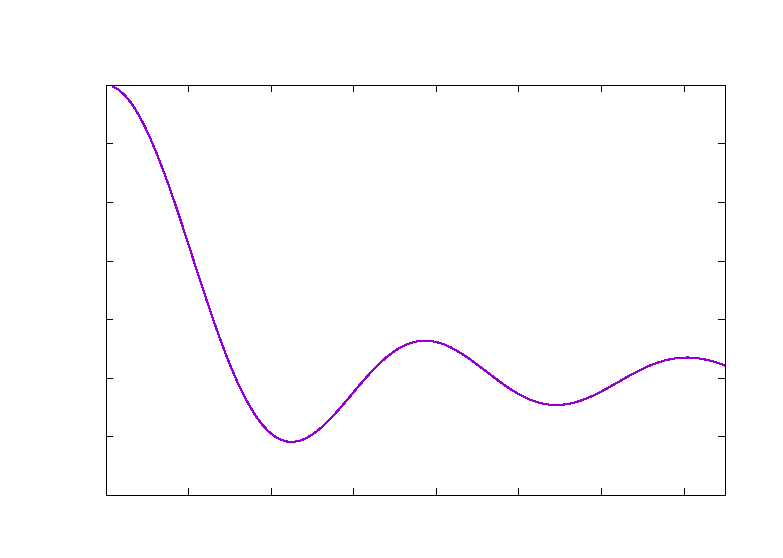
\includegraphics{r4}}%
    \gplfronttext
  \end{picture}%
\endgroup
}
%%%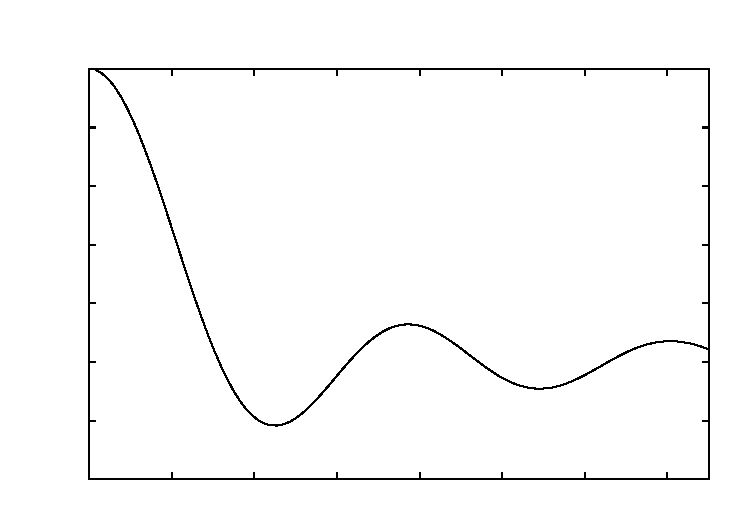
\includegraphics{../Images/ecc_plot/r4}
%%\end{figure}
%
%%\begin{figure}[h]
%%%\resizebox{2.5in}{!}{% GNUPLOT: LaTeX picture with Postscript
\begingroup
  \makeatletter
  \providecommand\color[2][]{%
    \GenericError{(gnuplot) \space\space\space\@spaces}{%
      Package color not loaded in conjunction with
      terminal option `colourtext'%
    }{See the gnuplot documentation for explanation.%
    }{Either use 'blacktext' in gnuplot or load the package
      color.sty in LaTeX.}%
    \renewcommand\color[2][]{}%
  }%
  \providecommand\includegraphics[2][]{%
    \GenericError{(gnuplot) \space\space\space\@spaces}{%
      Package graphicx or graphics not loaded%
    }{See the gnuplot documentation for explanation.%
    }{The gnuplot epslatex terminal needs graphicx.sty or graphics.sty.}%
    \renewcommand\includegraphics[2][]{}%
  }%
  \providecommand\rotatebox[2]{#2}%
  \@ifundefined{ifGPcolor}{%
    \newif\ifGPcolor
    \GPcolorfalse
  }{}%
  \@ifundefined{ifGPblacktext}{%
    \newif\ifGPblacktext
    \GPblacktexttrue
  }{}%
  % define a \g@addto@macro without @ in the name:
  \let\gplgaddtomacro\g@addto@macro
  % define empty templates for all commands taking text:
  \gdef\gplbacktext{}%
  \gdef\gplfronttext{}%
  \makeatother
  \ifGPblacktext
    % no textcolor at all
    \def\colorrgb#1{}%
    \def\colorgray#1{}%
  \else
    % gray or color?
    \ifGPcolor
      \def\colorrgb#1{\color[rgb]{#1}}%
      \def\colorgray#1{\color[gray]{#1}}%
      \expandafter\def\csname LTw\endcsname{\color{white}}%
      \expandafter\def\csname LTb\endcsname{\color{black}}%
      \expandafter\def\csname LTa\endcsname{\color{black}}%
      \expandafter\def\csname LT0\endcsname{\color[rgb]{1,0,0}}%
      \expandafter\def\csname LT1\endcsname{\color[rgb]{0,1,0}}%
      \expandafter\def\csname LT2\endcsname{\color[rgb]{0,0,1}}%
      \expandafter\def\csname LT3\endcsname{\color[rgb]{1,0,1}}%
      \expandafter\def\csname LT4\endcsname{\color[rgb]{0,1,1}}%
      \expandafter\def\csname LT5\endcsname{\color[rgb]{1,1,0}}%
      \expandafter\def\csname LT6\endcsname{\color[rgb]{0,0,0}}%
      \expandafter\def\csname LT7\endcsname{\color[rgb]{1,0.3,0}}%
      \expandafter\def\csname LT8\endcsname{\color[rgb]{0.5,0.5,0.5}}%
    \else
      % gray
      \def\colorrgb#1{\color{black}}%
      \def\colorgray#1{\color[gray]{#1}}%
      \expandafter\def\csname LTw\endcsname{\color{white}}%
      \expandafter\def\csname LTb\endcsname{\color{black}}%
      \expandafter\def\csname LTa\endcsname{\color{black}}%
      \expandafter\def\csname LT0\endcsname{\color{black}}%
      \expandafter\def\csname LT1\endcsname{\color{black}}%
      \expandafter\def\csname LT2\endcsname{\color{black}}%
      \expandafter\def\csname LT3\endcsname{\color{black}}%
      \expandafter\def\csname LT4\endcsname{\color{black}}%
      \expandafter\def\csname LT5\endcsname{\color{black}}%
      \expandafter\def\csname LT6\endcsname{\color{black}}%
      \expandafter\def\csname LT7\endcsname{\color{black}}%
      \expandafter\def\csname LT8\endcsname{\color{black}}%
    \fi
  \fi
  \setlength{\unitlength}{0.0500bp}%
  \begin{picture}(7200.00,5040.00)%
    \gplgaddtomacro\gplbacktext{%
      \csname LTb\endcsname%
      \put(726,440){\makebox(0,0)[r]{\strut{}-0.4}}%
      \put(726,1003){\makebox(0,0)[r]{\strut{}-0.2}}%
      \put(726,1565){\makebox(0,0)[r]{\strut{} 0}}%
      \put(726,2128){\makebox(0,0)[r]{\strut{} 0.2}}%
      \put(726,2691){\makebox(0,0)[r]{\strut{} 0.4}}%
      \put(726,3254){\makebox(0,0)[r]{\strut{} 0.6}}%
      \put(726,3816){\makebox(0,0)[r]{\strut{} 0.8}}%
      \put(726,4379){\makebox(0,0)[r]{\strut{} 1}}%
      \put(858,220){\makebox(0,0){\strut{} 0}}%
      \put(1651,220){\makebox(0,0){\strut{} 2}}%
      \put(2443,220){\makebox(0,0){\strut{} 4}}%
      \put(3236,220){\makebox(0,0){\strut{} 6}}%
      \put(4029,220){\makebox(0,0){\strut{} 8}}%
      \put(4821,220){\makebox(0,0){\strut{} 10}}%
      \put(5614,220){\makebox(0,0){\strut{} 12}}%
      \put(6407,220){\makebox(0,0){\strut{} 14}}%
      \put(3830,4709){\makebox(0,0){\strut{}\Large Illustrating L’H\^opital’s Rule: $\frac{\sin(x)}{x}$}}%
      \put(4128,3394){\makebox(0,0)[l]{\strut{}\Large$\displaystyle \lim_{x\Longrightarrow0}\frac{\sin(x)}{x}=1$}}%
    }%
    \gplgaddtomacro\gplfronttext{%
    }%
    \gplbacktext
    \put(0,0){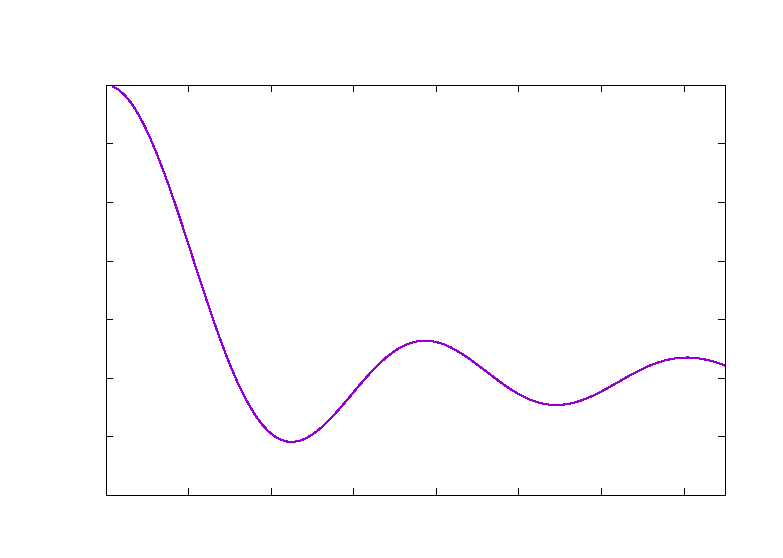
\includegraphics{r4}}%
    \gplfronttext
  \end{picture}%
\endgroup
}
%%%\scalebox{.5}{% GNUPLOT: LaTeX picture with Postscript
\begingroup
  \makeatletter
  \providecommand\color[2][]{%
    \GenericError{(gnuplot) \space\space\space\@spaces}{%
      Package color not loaded in conjunction with
      terminal option `colourtext'%
    }{See the gnuplot documentation for explanation.%
    }{Either use 'blacktext' in gnuplot or load the package
      color.sty in LaTeX.}%
    \renewcommand\color[2][]{}%
  }%
  \providecommand\includegraphics[2][]{%
    \GenericError{(gnuplot) \space\space\space\@spaces}{%
      Package graphicx or graphics not loaded%
    }{See the gnuplot documentation for explanation.%
    }{The gnuplot epslatex terminal needs graphicx.sty or graphics.sty.}%
    \renewcommand\includegraphics[2][]{}%
  }%
  \providecommand\rotatebox[2]{#2}%
  \@ifundefined{ifGPcolor}{%
    \newif\ifGPcolor
    \GPcolorfalse
  }{}%
  \@ifundefined{ifGPblacktext}{%
    \newif\ifGPblacktext
    \GPblacktexttrue
  }{}%
  % define a \g@addto@macro without @ in the name:
  \let\gplgaddtomacro\g@addto@macro
  % define empty templates for all commands taking text:
  \gdef\gplbacktext{}%
  \gdef\gplfronttext{}%
  \makeatother
  \ifGPblacktext
    % no textcolor at all
    \def\colorrgb#1{}%
    \def\colorgray#1{}%
  \else
    % gray or color?
    \ifGPcolor
      \def\colorrgb#1{\color[rgb]{#1}}%
      \def\colorgray#1{\color[gray]{#1}}%
      \expandafter\def\csname LTw\endcsname{\color{white}}%
      \expandafter\def\csname LTb\endcsname{\color{black}}%
      \expandafter\def\csname LTa\endcsname{\color{black}}%
      \expandafter\def\csname LT0\endcsname{\color[rgb]{1,0,0}}%
      \expandafter\def\csname LT1\endcsname{\color[rgb]{0,1,0}}%
      \expandafter\def\csname LT2\endcsname{\color[rgb]{0,0,1}}%
      \expandafter\def\csname LT3\endcsname{\color[rgb]{1,0,1}}%
      \expandafter\def\csname LT4\endcsname{\color[rgb]{0,1,1}}%
      \expandafter\def\csname LT5\endcsname{\color[rgb]{1,1,0}}%
      \expandafter\def\csname LT6\endcsname{\color[rgb]{0,0,0}}%
      \expandafter\def\csname LT7\endcsname{\color[rgb]{1,0.3,0}}%
      \expandafter\def\csname LT8\endcsname{\color[rgb]{0.5,0.5,0.5}}%
    \else
      % gray
      \def\colorrgb#1{\color{black}}%
      \def\colorgray#1{\color[gray]{#1}}%
      \expandafter\def\csname LTw\endcsname{\color{white}}%
      \expandafter\def\csname LTb\endcsname{\color{black}}%
      \expandafter\def\csname LTa\endcsname{\color{black}}%
      \expandafter\def\csname LT0\endcsname{\color{black}}%
      \expandafter\def\csname LT1\endcsname{\color{black}}%
      \expandafter\def\csname LT2\endcsname{\color{black}}%
      \expandafter\def\csname LT3\endcsname{\color{black}}%
      \expandafter\def\csname LT4\endcsname{\color{black}}%
      \expandafter\def\csname LT5\endcsname{\color{black}}%
      \expandafter\def\csname LT6\endcsname{\color{black}}%
      \expandafter\def\csname LT7\endcsname{\color{black}}%
      \expandafter\def\csname LT8\endcsname{\color{black}}%
    \fi
  \fi
  \setlength{\unitlength}{0.0500bp}%
  \begin{picture}(7200.00,5040.00)%
    \gplgaddtomacro\gplbacktext{%
      \csname LTb\endcsname%
      \put(726,440){\makebox(0,0)[r]{\strut{}-0.4}}%
      \put(726,1003){\makebox(0,0)[r]{\strut{}-0.2}}%
      \put(726,1565){\makebox(0,0)[r]{\strut{} 0}}%
      \put(726,2128){\makebox(0,0)[r]{\strut{} 0.2}}%
      \put(726,2691){\makebox(0,0)[r]{\strut{} 0.4}}%
      \put(726,3254){\makebox(0,0)[r]{\strut{} 0.6}}%
      \put(726,3816){\makebox(0,0)[r]{\strut{} 0.8}}%
      \put(726,4379){\makebox(0,0)[r]{\strut{} 1}}%
      \put(858,220){\makebox(0,0){\strut{} 0}}%
      \put(1651,220){\makebox(0,0){\strut{} 2}}%
      \put(2443,220){\makebox(0,0){\strut{} 4}}%
      \put(3236,220){\makebox(0,0){\strut{} 6}}%
      \put(4029,220){\makebox(0,0){\strut{} 8}}%
      \put(4821,220){\makebox(0,0){\strut{} 10}}%
      \put(5614,220){\makebox(0,0){\strut{} 12}}%
      \put(6407,220){\makebox(0,0){\strut{} 14}}%
      \put(3830,4709){\makebox(0,0){\strut{}\Large Illustrating L’H\^opital’s Rule: $\frac{\sin(x)}{x}$}}%
      \put(4128,3394){\makebox(0,0)[l]{\strut{}\Large$\displaystyle \lim_{x\Longrightarrow0}\frac{\sin(x)}{x}=1$}}%
    }%
    \gplgaddtomacro\gplfronttext{%
    }%
    \gplbacktext
    \put(0,0){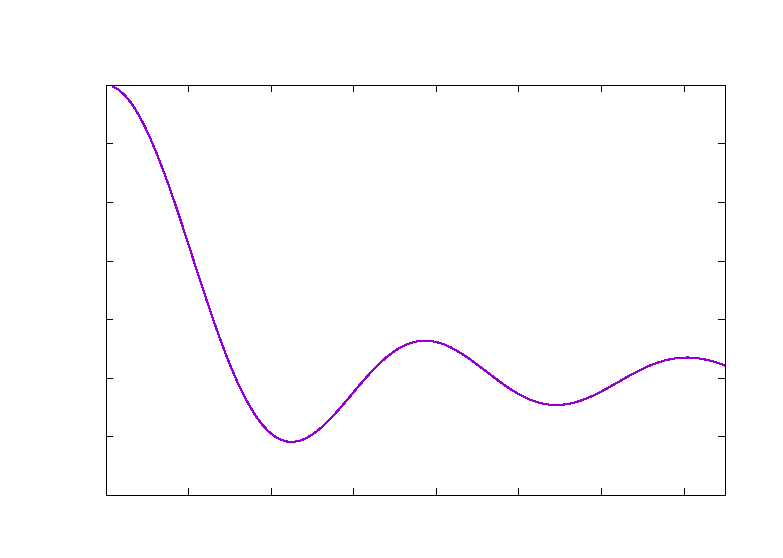
\includegraphics{r4}}%
    \gplfronttext
  \end{picture}%
\endgroup
}
%%%\scalebox{.5}{% GNUPLOT: LaTeX picture with Postscript
\begingroup
  \makeatletter
  \providecommand\color[2][]{%
    \GenericError{(gnuplot) \space\space\space\@spaces}{%
      Package color not loaded in conjunction with
      terminal option `colourtext'%
    }{See the gnuplot documentation for explanation.%
    }{Either use 'blacktext' in gnuplot or load the package
      color.sty in LaTeX.}%
    \renewcommand\color[2][]{}%
  }%
  \providecommand\includegraphics[2][]{%
    \GenericError{(gnuplot) \space\space\space\@spaces}{%
      Package graphicx or graphics not loaded%
    }{See the gnuplot documentation for explanation.%
    }{The gnuplot epslatex terminal needs graphicx.sty or graphics.sty.}%
    \renewcommand\includegraphics[2][]{}%
  }%
  \providecommand\rotatebox[2]{#2}%
  \@ifundefined{ifGPcolor}{%
    \newif\ifGPcolor
    \GPcolorfalse
  }{}%
  \@ifundefined{ifGPblacktext}{%
    \newif\ifGPblacktext
    \GPblacktexttrue
  }{}%
  % define a \g@addto@macro without @ in the name:
  \let\gplgaddtomacro\g@addto@macro
  % define empty templates for all commands taking text:
  \gdef\gplbacktext{}%
  \gdef\gplfronttext{}%
  \makeatother
  \ifGPblacktext
    % no textcolor at all
    \def\colorrgb#1{}%
    \def\colorgray#1{}%
  \else
    % gray or color?
    \ifGPcolor
      \def\colorrgb#1{\color[rgb]{#1}}%
      \def\colorgray#1{\color[gray]{#1}}%
      \expandafter\def\csname LTw\endcsname{\color{white}}%
      \expandafter\def\csname LTb\endcsname{\color{black}}%
      \expandafter\def\csname LTa\endcsname{\color{black}}%
      \expandafter\def\csname LT0\endcsname{\color[rgb]{1,0,0}}%
      \expandafter\def\csname LT1\endcsname{\color[rgb]{0,1,0}}%
      \expandafter\def\csname LT2\endcsname{\color[rgb]{0,0,1}}%
      \expandafter\def\csname LT3\endcsname{\color[rgb]{1,0,1}}%
      \expandafter\def\csname LT4\endcsname{\color[rgb]{0,1,1}}%
      \expandafter\def\csname LT5\endcsname{\color[rgb]{1,1,0}}%
      \expandafter\def\csname LT6\endcsname{\color[rgb]{0,0,0}}%
      \expandafter\def\csname LT7\endcsname{\color[rgb]{1,0.3,0}}%
      \expandafter\def\csname LT8\endcsname{\color[rgb]{0.5,0.5,0.5}}%
    \else
      % gray
      \def\colorrgb#1{\color{black}}%
      \def\colorgray#1{\color[gray]{#1}}%
      \expandafter\def\csname LTw\endcsname{\color{white}}%
      \expandafter\def\csname LTb\endcsname{\color{black}}%
      \expandafter\def\csname LTa\endcsname{\color{black}}%
      \expandafter\def\csname LT0\endcsname{\color{black}}%
      \expandafter\def\csname LT1\endcsname{\color{black}}%
      \expandafter\def\csname LT2\endcsname{\color{black}}%
      \expandafter\def\csname LT3\endcsname{\color{black}}%
      \expandafter\def\csname LT4\endcsname{\color{black}}%
      \expandafter\def\csname LT5\endcsname{\color{black}}%
      \expandafter\def\csname LT6\endcsname{\color{black}}%
      \expandafter\def\csname LT7\endcsname{\color{black}}%
      \expandafter\def\csname LT8\endcsname{\color{black}}%
    \fi
  \fi
  \setlength{\unitlength}{0.0500bp}%
  \begin{picture}(7200.00,5040.00)%
    \gplgaddtomacro\gplbacktext{%
      \csname LTb\endcsname%
      \put(726,440){\makebox(0,0)[r]{\strut{}-0.4}}%
      \put(726,1003){\makebox(0,0)[r]{\strut{}-0.2}}%
      \put(726,1565){\makebox(0,0)[r]{\strut{} 0}}%
      \put(726,2128){\makebox(0,0)[r]{\strut{} 0.2}}%
      \put(726,2691){\makebox(0,0)[r]{\strut{} 0.4}}%
      \put(726,3254){\makebox(0,0)[r]{\strut{} 0.6}}%
      \put(726,3816){\makebox(0,0)[r]{\strut{} 0.8}}%
      \put(726,4379){\makebox(0,0)[r]{\strut{} 1}}%
      \put(858,220){\makebox(0,0){\strut{} 0}}%
      \put(1651,220){\makebox(0,0){\strut{} 2}}%
      \put(2443,220){\makebox(0,0){\strut{} 4}}%
      \put(3236,220){\makebox(0,0){\strut{} 6}}%
      \put(4029,220){\makebox(0,0){\strut{} 8}}%
      \put(4821,220){\makebox(0,0){\strut{} 10}}%
      \put(5614,220){\makebox(0,0){\strut{} 12}}%
      \put(6407,220){\makebox(0,0){\strut{} 14}}%
      \put(3830,4709){\makebox(0,0){\strut{}\Large Illustrating L’H\^opital’s Rule: $\frac{\sin(x)}{x}$}}%
      \put(4128,3394){\makebox(0,0)[l]{\strut{}\Large$\displaystyle \lim_{x\Longrightarrow0}\frac{\sin(x)}{x}=1$}}%
    }%
    \gplgaddtomacro\gplfronttext{%
    }%
    \gplbacktext
    \put(0,0){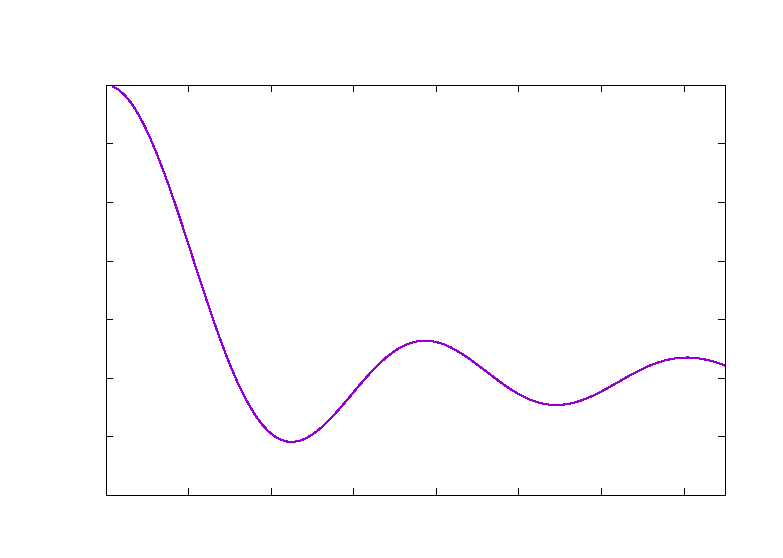
\includegraphics{r4}}%
    \gplfronttext
  \end{picture}%
\endgroup
}
%%%\scalebox{.5}{% GNUPLOT: LaTeX picture with Postscript
\begingroup
  \makeatletter
  \providecommand\color[2][]{%
    \GenericError{(gnuplot) \space\space\space\@spaces}{%
      Package color not loaded in conjunction with
      terminal option `colourtext'%
    }{See the gnuplot documentation for explanation.%
    }{Either use 'blacktext' in gnuplot or load the package
      color.sty in LaTeX.}%
    \renewcommand\color[2][]{}%
  }%
  \providecommand\includegraphics[2][]{%
    \GenericError{(gnuplot) \space\space\space\@spaces}{%
      Package graphicx or graphics not loaded%
    }{See the gnuplot documentation for explanation.%
    }{The gnuplot epslatex terminal needs graphicx.sty or graphics.sty.}%
    \renewcommand\includegraphics[2][]{}%
  }%
  \providecommand\rotatebox[2]{#2}%
  \@ifundefined{ifGPcolor}{%
    \newif\ifGPcolor
    \GPcolorfalse
  }{}%
  \@ifundefined{ifGPblacktext}{%
    \newif\ifGPblacktext
    \GPblacktexttrue
  }{}%
  % define a \g@addto@macro without @ in the name:
  \let\gplgaddtomacro\g@addto@macro
  % define empty templates for all commands taking text:
  \gdef\gplbacktext{}%
  \gdef\gplfronttext{}%
  \makeatother
  \ifGPblacktext
    % no textcolor at all
    \def\colorrgb#1{}%
    \def\colorgray#1{}%
  \else
    % gray or color?
    \ifGPcolor
      \def\colorrgb#1{\color[rgb]{#1}}%
      \def\colorgray#1{\color[gray]{#1}}%
      \expandafter\def\csname LTw\endcsname{\color{white}}%
      \expandafter\def\csname LTb\endcsname{\color{black}}%
      \expandafter\def\csname LTa\endcsname{\color{black}}%
      \expandafter\def\csname LT0\endcsname{\color[rgb]{1,0,0}}%
      \expandafter\def\csname LT1\endcsname{\color[rgb]{0,1,0}}%
      \expandafter\def\csname LT2\endcsname{\color[rgb]{0,0,1}}%
      \expandafter\def\csname LT3\endcsname{\color[rgb]{1,0,1}}%
      \expandafter\def\csname LT4\endcsname{\color[rgb]{0,1,1}}%
      \expandafter\def\csname LT5\endcsname{\color[rgb]{1,1,0}}%
      \expandafter\def\csname LT6\endcsname{\color[rgb]{0,0,0}}%
      \expandafter\def\csname LT7\endcsname{\color[rgb]{1,0.3,0}}%
      \expandafter\def\csname LT8\endcsname{\color[rgb]{0.5,0.5,0.5}}%
    \else
      % gray
      \def\colorrgb#1{\color{black}}%
      \def\colorgray#1{\color[gray]{#1}}%
      \expandafter\def\csname LTw\endcsname{\color{white}}%
      \expandafter\def\csname LTb\endcsname{\color{black}}%
      \expandafter\def\csname LTa\endcsname{\color{black}}%
      \expandafter\def\csname LT0\endcsname{\color{black}}%
      \expandafter\def\csname LT1\endcsname{\color{black}}%
      \expandafter\def\csname LT2\endcsname{\color{black}}%
      \expandafter\def\csname LT3\endcsname{\color{black}}%
      \expandafter\def\csname LT4\endcsname{\color{black}}%
      \expandafter\def\csname LT5\endcsname{\color{black}}%
      \expandafter\def\csname LT6\endcsname{\color{black}}%
      \expandafter\def\csname LT7\endcsname{\color{black}}%
      \expandafter\def\csname LT8\endcsname{\color{black}}%
    \fi
  \fi
  \setlength{\unitlength}{0.0500bp}%
  \begin{picture}(7200.00,5040.00)%
    \gplgaddtomacro\gplbacktext{%
      \csname LTb\endcsname%
      \put(726,440){\makebox(0,0)[r]{\strut{}-0.4}}%
      \put(726,1003){\makebox(0,0)[r]{\strut{}-0.2}}%
      \put(726,1565){\makebox(0,0)[r]{\strut{} 0}}%
      \put(726,2128){\makebox(0,0)[r]{\strut{} 0.2}}%
      \put(726,2691){\makebox(0,0)[r]{\strut{} 0.4}}%
      \put(726,3254){\makebox(0,0)[r]{\strut{} 0.6}}%
      \put(726,3816){\makebox(0,0)[r]{\strut{} 0.8}}%
      \put(726,4379){\makebox(0,0)[r]{\strut{} 1}}%
      \put(858,220){\makebox(0,0){\strut{} 0}}%
      \put(1651,220){\makebox(0,0){\strut{} 2}}%
      \put(2443,220){\makebox(0,0){\strut{} 4}}%
      \put(3236,220){\makebox(0,0){\strut{} 6}}%
      \put(4029,220){\makebox(0,0){\strut{} 8}}%
      \put(4821,220){\makebox(0,0){\strut{} 10}}%
      \put(5614,220){\makebox(0,0){\strut{} 12}}%
      \put(6407,220){\makebox(0,0){\strut{} 14}}%
      \put(3830,4709){\makebox(0,0){\strut{}\Large Illustrating L’H\^opital’s Rule: $\frac{\sin(x)}{x}$}}%
      \put(4128,3394){\makebox(0,0)[l]{\strut{}\Large$\displaystyle \lim_{x\Longrightarrow0}\frac{\sin(x)}{x}=1$}}%
    }%
    \gplgaddtomacro\gplfronttext{%
    }%
    \gplbacktext
    \put(0,0){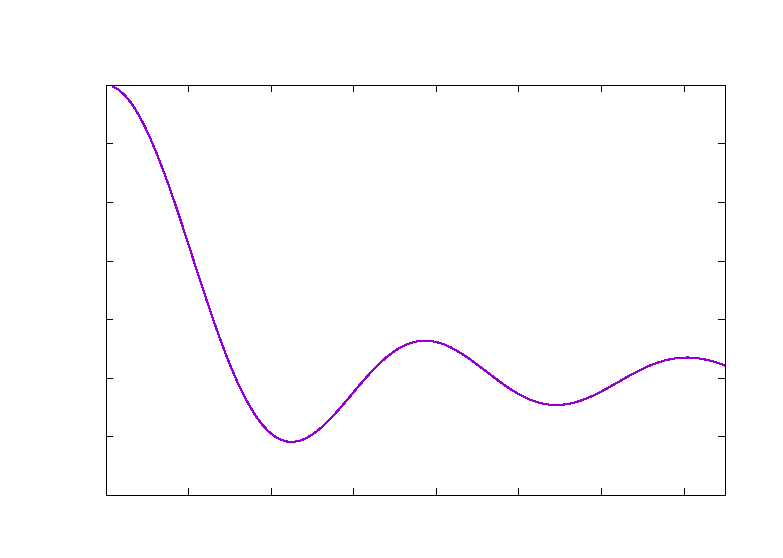
\includegraphics{r4}}%
    \gplfronttext
  \end{picture}%
\endgroup
}
%%\includegraphics{../Images/ecc_plot/ecc_2_3}
%%\end{figure}
%%
%%\begin{figure}[!htbp]
%%\begin{minipage}{0.3\textwidth} \centering
%%\includegraphics{../Images/ecc_plot/ecc_2_3} 
%%%\caption{图表1}
%%\end{minipage}
%%\begin{minipage}{0.3\textwidth} \centering
%%\includegraphics{../Images/ecc_plot/ecc_2_3} 
%%%\caption{图表2}
%%\end{minipage}
%%\begin{minipage}{0.3\textwidth} \centering
%%\includegraphics{../Images/ecc_plot/ecc_2_3} 
%%%\caption{图表3}
%%\end{minipage}
%%\end{figure}
%%\begin{figure}[!htbp]
%%\begin{minipage}{0.3\textwidth} \centering
%%\includegraphics{../Images/ecc_plot/ecc_2_3} 
%%%\caption{图表1}
%%\end{minipage}
%%\begin{minipage}{0.3\textwidth} \centering
%%\includegraphics{../Images/ecc_plot/ecc_2_3} 
%%%\caption{图表2}
%%\end{minipage}
%%\begin{minipage}{0.3\textwidth} \centering
%%\includegraphics{../Images/ecc_plot/ecc_2_3} 
%%%\caption{图表3}
%%\end{minipage}
%%\end{figure}
%%
%%Some text in this section. And here we insert the picture:
%%\begin{figure}[H]
%%  \centering
%%  \includegraphics{../Images/ecc_plot/ecc_2_3}
%%  \caption{This is the inserted picture.}
%%\end{figure}
%%More text after the picture.
%
%The Black-Scholes model is a fundamental tool in financial markets for pricing options. It provides insights into the behavior of option prices and the factors that affect them. Understanding the model and its derivations is crucial for anyone involved in finance.
%

\end{document}
